% Options for packages loaded elsewhere
\PassOptionsToPackage{unicode}{hyperref}
\PassOptionsToPackage{hyphens}{url}
\PassOptionsToPackage{dvipsnames,svgnames,x11names}{xcolor}
%
\documentclass[
  12pt]{article}

\usepackage{amsmath,amssymb}
\usepackage{iftex}
\ifPDFTeX
  \usepackage[T1]{fontenc}
  \usepackage[utf8]{inputenc}
  \usepackage{textcomp} % provide euro and other symbols
\else % if luatex or xetex
  \usepackage{unicode-math}
  \defaultfontfeatures{Scale=MatchLowercase}
  \defaultfontfeatures[\rmfamily]{Ligatures=TeX,Scale=1}
\fi
\usepackage{lmodern}
\ifPDFTeX\else  
    % xetex/luatex font selection
\fi
% Use upquote if available, for straight quotes in verbatim environments
\IfFileExists{upquote.sty}{\usepackage{upquote}}{}
\IfFileExists{microtype.sty}{% use microtype if available
  \usepackage[]{microtype}
  \UseMicrotypeSet[protrusion]{basicmath} % disable protrusion for tt fonts
}{}
\makeatletter
\@ifundefined{KOMAClassName}{% if non-KOMA class
  \IfFileExists{parskip.sty}{%
    \usepackage{parskip}
  }{% else
    \setlength{\parindent}{0pt}
    \setlength{\parskip}{6pt plus 2pt minus 1pt}}
}{% if KOMA class
  \KOMAoptions{parskip=half}}
\makeatother
\usepackage{xcolor}
\setlength{\emergencystretch}{3em} % prevent overfull lines
\setcounter{secnumdepth}{5}
% Make \paragraph and \subparagraph free-standing
\ifx\paragraph\undefined\else
  \let\oldparagraph\paragraph
  \renewcommand{\paragraph}[1]{\oldparagraph{#1}\mbox{}}
\fi
\ifx\subparagraph\undefined\else
  \let\oldsubparagraph\subparagraph
  \renewcommand{\subparagraph}[1]{\oldsubparagraph{#1}\mbox{}}
\fi


\providecommand{\tightlist}{%
  \setlength{\itemsep}{0pt}\setlength{\parskip}{0pt}}\usepackage{longtable,booktabs,array}
\usepackage{calc} % for calculating minipage widths
% Correct order of tables after \paragraph or \subparagraph
\usepackage{etoolbox}
\makeatletter
\patchcmd\longtable{\par}{\if@noskipsec\mbox{}\fi\par}{}{}
\makeatother
% Allow footnotes in longtable head/foot
\IfFileExists{footnotehyper.sty}{\usepackage{footnotehyper}}{\usepackage{footnote}}
\makesavenoteenv{longtable}
\usepackage{graphicx}
\makeatletter
\def\maxwidth{\ifdim\Gin@nat@width>\linewidth\linewidth\else\Gin@nat@width\fi}
\def\maxheight{\ifdim\Gin@nat@height>\textheight\textheight\else\Gin@nat@height\fi}
\makeatother
% Scale images if necessary, so that they will not overflow the page
% margins by default, and it is still possible to overwrite the defaults
% using explicit options in \includegraphics[width, height, ...]{}
\setkeys{Gin}{width=\maxwidth,height=\maxheight,keepaspectratio}
% Set default figure placement to htbp
\makeatletter
\def\fps@figure{htbp}
\makeatother

\addtolength{\oddsidemargin}{-.5in}%
\addtolength{\evensidemargin}{-1in}%
\addtolength{\textwidth}{1in}%
\addtolength{\textheight}{1.7in}%
\addtolength{\topmargin}{-1in}%

\usepackage{amsthm}
\newtheorem{ass}{Assumption}
% \usepackage{mathtools}
\usepackage[draft, nomargin, inline, nomarginclue, author=HM]{fixme}
% \fxusetargetlayout{color}
\fxsetface{inline}{\color{blue}}
\fxsetface{env}{\color{blue}}
% \usepackage{amsmath}
% \usepackage[final,nomargin,index,inline, author=]{fixme}
% \usepackage{bbm}
\usepackage{unicode-math}
\usepackage{tabularx}
\usepackage{adjustbox}
% \usepackage{amsmath}
% - \usepackage{longtable}
% - \usepackage{booktabs}
% - \usepackage{graphicx}
% \newtheorem{definition}{Definition}
% \newtheorem{theo}{Theorem}
% \newtheorem{lemma}{Lemma}
% \newtheorem{ass}{Assumption}
% \usepackage{xkvltxp}
% -  #final or draft
% - \fxsetup{envlayout=color, targetlayout=color}
% - \fxsetface{inline}{\color{blue}}

% kableExtra required packages:
\usepackage{booktabs}
\usepackage{longtable}
% \usepackage{array}
% \usepackage{multirow}
% \usepackage{wrapfig}
% \usepackage{float}
% \usepackage{colortbl}
% \usepackage{pdflscape}
% \usepackage{tabu}
\usepackage{threeparttable}
\usepackage{threeparttablex}
% \usepackage[normalem]{ulem}
% \usepackage{makecell}
% \usepackage{xcolor}
\usepackage{booktabs}
\usepackage{longtable}
\usepackage{array}
\usepackage{multirow}
\usepackage{wrapfig}
\usepackage{float}
\usepackage{colortbl}
\usepackage{pdflscape}
\usepackage{tabu}
\usepackage{threeparttable}
\usepackage{threeparttablex}
\usepackage[normalem]{ulem}
\usepackage{makecell}
\usepackage{xcolor}
\usepackage{tabularray}
\usepackage[normalem]{ulem}
\usepackage{graphicx}
\UseTblrLibrary{booktabs}
\UseTblrLibrary{siunitx}
\NewTableCommand{\tinytableDefineColor}[3]{\definecolor{#1}{#2}{#3}}
\newcommand{\tinytableTabularrayUnderline}[1]{\underline{#1}}
\newcommand{\tinytableTabularrayStrikeout}[1]{\sout{#1}}
\makeatletter
\@ifpackageloaded{caption}{}{\usepackage{caption}}
\AtBeginDocument{%
\ifdefined\contentsname
  \renewcommand*\contentsname{Table of contents}
\else
  \newcommand\contentsname{Table of contents}
\fi
\ifdefined\listfigurename
  \renewcommand*\listfigurename{List of Figures}
\else
  \newcommand\listfigurename{List of Figures}
\fi
\ifdefined\listtablename
  \renewcommand*\listtablename{List of Tables}
\else
  \newcommand\listtablename{List of Tables}
\fi
\ifdefined\figurename
  \renewcommand*\figurename{Figure}
\else
  \newcommand\figurename{Figure}
\fi
\ifdefined\tablename
  \renewcommand*\tablename{Table}
\else
  \newcommand\tablename{Table}
\fi
}
\@ifpackageloaded{float}{}{\usepackage{float}}
\floatstyle{ruled}
\@ifundefined{c@chapter}{\newfloat{codelisting}{h}{lop}}{\newfloat{codelisting}{h}{lop}[chapter]}
\floatname{codelisting}{Listing}
\newcommand*\listoflistings{\listof{codelisting}{List of Listings}}
\usepackage{amsthm}
\theoremstyle{definition}
\newtheorem{definition}{Definition}[section]
\theoremstyle{remark}
\AtBeginDocument{\renewcommand*{\proofname}{Proof}}
\newtheorem*{remark}{Remark}
\newtheorem*{solution}{Solution}
\newtheorem{refremark}{Remark}[section]
\newtheorem{refsolution}{Solution}[section]
\makeatother
\makeatletter
\makeatother
\makeatletter
\@ifpackageloaded{caption}{}{\usepackage{caption}}
\@ifpackageloaded{subcaption}{}{\usepackage{subcaption}}
\makeatother
\makeatletter
\@ifpackageloaded{tcolorbox}{}{\usepackage[many]{tcolorbox}}
\makeatother
%%%% ---foldboxy preamble ----- %%%%%

\definecolor{fbx-default-color1}{HTML}{c7c7d0}
\definecolor{fbx-default-color2}{HTML}{a3a3aa}

\definecolor{fbox-color1}{HTML}{c7c7d0}
\definecolor{fbox-color2}{HTML}{a3a3aa}

% arguments: #1 typelabelnummer: #2 titel: #3
\newenvironment{fbx}[3]{\begin{tcolorbox}[enhanced, breakable,%
attach boxed title to top*={xshift=1.4pt},
boxed title style={boxrule=0.0mm, fuzzy shadow={1pt}{-1pt}{0mm}{0.1mm}{gray}, arc=.3em, rounded corners=east, sharp corners=west}, colframe=#1-color2, colbacktitle=#1-color1, colback = white, coltitle=black,  titlerule=0mm, toprule=0pt, bottomrule=.7pt, leftrule=.3em, rightrule=0pt, outer arc=.3em,  arc=0pt,	 sharp corners = east, left=.5em, bottomtitle=1mm, toptitle=1mm,title=\textbf{#2}\hspace{0.5em}{#3}]}
{\end{tcolorbox}}

% boxed environment with right border
\newenvironment{fbxSimple}[3]{\begin{tcolorbox}[enhanced, breakable,%
attach boxed title to top*={xshift=1.4pt},
boxed title style={boxrule=0.0mm, fuzzy shadow={1pt}{-1pt}{0mm}{0.1mm}{gray}, arc=.3em, rounded corners=east, sharp corners=west}, colframe=#1-color2, colbacktitle=#1-color1, colback = white, coltitle=black,  titlerule=0mm, toprule=0pt, bottomrule=.7pt, leftrule=.3em, rightrule=.7pt, outer arc=.3em,  	left=.5em, right=.5em, bottomtitle=1mm, toptitle=1mm,title=\textbf{#2}\hspace{0.5em}{#3}]}
{\end{tcolorbox}}

%%%% --- end foldboxy preamble ----- %%%%%
%%==== colors from yaml ===%
\definecolor{Proposition-color1}{HTML}{99CCFF}
\definecolor{Proposition-color2}{HTML}{FFFFFF}
\definecolor{Assumption-color1}{HTML}{99CCFF}
\definecolor{Assumption-color2}{HTML}{FFFFFF}
\definecolor{Theorem-color1}{HTML}{99CCFF}
\definecolor{Theorem-color2}{HTML}{FFFFFF}
\definecolor{Definition-color1}{HTML}{99CCFF}
\definecolor{Definition-color2}{HTML}{FFFFFF}
%=============%
\ifLuaTeX
  \usepackage{selnolig}  % disable illegal ligatures
\fi
\usepackage[]{natbib}
\bibliographystyle{agsm}
\usepackage{bookmark}

\IfFileExists{xurl.sty}{\usepackage{xurl}}{} % add URL line breaks if available
\urlstyle{same} % disable monospaced font for URLs
\hypersetup{
  pdftitle={Tax Evasion and Productivity},
  pdfauthor={Hans Martinez},
  pdfkeywords={Tax Evasion, Cost Overreporting, Production Function
Estimation, Productivity},
  colorlinks=true,
  linkcolor={blue},
  filecolor={Maroon},
  citecolor={Blue},
  urlcolor={Blue},
  pdfcreator={LaTeX via pandoc}}


\begin{document}


\def\spacingset#1{\renewcommand{\baselinestretch}%
{#1}\small\normalsize} \spacingset{1}


%%%%%%%%%%%%%%%%%%%%%%%%%%%%%%%%%%%%%%%%%%%%%%%%%%%%%%%%%%%%%%%%%%%%%%%%%%%%%%

\date{September 11, 2025}
\title{\bf Tax Evasion and Productivity}
\author{
Hans Martinez\thanks{email: hmarti33@uwo.ca.}\\
Department of Economics, University of Western Ontario\\
}
\maketitle

\bigskip
\bigskip
\begin{abstract}
I propose a novel strategy that uses production functions to estimate
corporate tax evasion through cost overreporting. Employing a structural
production function approach using validation data with correctly
reported costs, I investigate potential tax evasion by testing the
presence of cost overreporting on a testing data, where the
statistically significant differences on the output elasticities of the
overreported input in the correct direction are interpreted as evidence
of tax evasion. I apply this method to a well-known dataset where I find
evidence suggesting that cost overreporting is widespread and
quantitatively large. My results indicate that ignoring cost
overreporting leads to consistently larger elasticities of intermediate
inputs. The bias on the intermediate inputs spreads to the elasticities
of labor and capital, whose bias direction varies by industry. Finally,
I find significant differences in the productivity distributions. How
much cheating there could be (back-of-envelope calculation, be careful
\end{abstract}

\noindent%
{\it Keywords:} Tax Evasion, Cost Overreporting, Production Function
Estimation, Productivity
\vfill

\newpage
\spacingset{1.9} % DON'T change the spacing!

\renewcommand*\contentsname{Table of contents}
{
\hypersetup{linkcolor=}
\setcounter{tocdepth}{3}
\tableofcontents
}
\section*{Introduction}\label{introduction}
\addcontentsline{toc}{section}{Introduction}

\begin{anfxnote}{Remove. Do not copy-paste abstract.}
I propose a novel method to estimate corporate tax evasion through cost
overreporting using production functions. I first show how that cost
overreporting lead to biased estimates of productivity and production
function parameters. Then, I show how to recover unbiased estimates of
the production function and productivity in the presence of tax evasion.
With the production function parameters and productivity on hand, the
production function can be inverted to recover the true inputs. Then, I
estimate cost overreporting as the difference between observed and true
inputs. I apply this method to a well-known dataset where I find
evidence suggesting that cost overreporting is widespread and
quantitatively large. I also find that ignoring cost overreporting leads
to consistently larger elasticities of intermediate inputs. The bias on
the intermediate inputs spreads to the elasticities of labor and
capital, whose bias direction varies by industry. Finally, I find
significant differences in the productivity distributions.

\end{anfxnote}

\fxnote{Title:What is cost overreporting?} Cost overreporting arises
when firms acquire false invoices to claim additional tax deductions on
value-added (VAT) and corporate income taxes (CIT). According to the
OECD's document \citet{OECD2017}, cost overreporting --- also known as
``fake invoicing'', ``ghost firms'', ``invoice mills'', or ``missing
traders''--- permeates internationally.

\fxnote{Title:Why do we care? Revenue losses for govt's} Reports from
Latin America, Eastern Europe, Asia, and Africa claim cost overreporting
led to annual tax revenue losses as large as 5.6\% of the GDP, for
example, in Poland, 2016 (Poland's Minister of Finance, 2018). Other
reports show that cost overreporting led to revenue losses of 0.2\% of
Chile's GDP in 2004 (Gonzalez and Velasquez, 2013; Jorrat, 2001; CIAT,
2008); 0.2\% of Colombia's GDP (Portafolio, 2019); and 0.03\% of
Mexico's GDP in 2018 (Senado de la Republica, 2019). \fxnote{Replace
percentages of GDP with USD. I care about Tax Revenue more than GDP. How
much am I losing in tax revenue? Throw Poland. Don't say ``up to''. Give
people a range. Compared to total tax revenue and the whole size of the
economy GDP. 20-30\% Tax Revenue relative to GDP.}

\fxnote{Title:Why do we care? Productivity biases} Furthermore, ignoring
tax evasion leads to biased estimates of productivity. In the proxy
variable literature, productivity is measured as the residual of the
production function, where the output of a firm is a function of the
inputs, capital, labor, and intermediates. A key assumption is that
intermediate input demand is strictly monotonic on the productivity of
the firm \citep{Gandhi2020, Ackerberg2015, Levinsohn2003}. In other
words, we expect highly productive firms will use fewer inputs to
produce a given level of output. Intermediate inputs, however, are also
the most likely input to be misreported. When firms overreport their
inputs increasing their costs to claim additional tax deductions, their
reported inputs are higher than their actual utilization, resulting in
lower productivity estimates.

\fxnote{Title:Overlooked by corp tax ev lit? Why?} Despite its
relevance, the literature on corporate tax evasion has mostly overlooked
cost overreporting. The few studies focusing on this tax evasion
strategy rely on exploiting detailed administrative data
\citep{Zumaya2021, Carrillo2022}. Due to firms' confidentiality
concerns, government tax authorities restrict access to kind of data. My
approach complements these methods. It is not restricted to confidential
tax records and can be applied using more commonly available data such
as firm-level surveys.

\fxnote{Title: Why is it hard?} To the best of my knowledge, no other
study has attempted to structurally identify cost overreporting. A
fundamental problem is that when it comes to corporate tax evasion,
researchers have to account for an additional source of unobserved
heterogeneity, productivity. Why? Because cost overreporting might be
naively quantified as low productivity. Intuitively, for a given output
level, high input utilization by a firm could be explained by either the
amount of input the firm overreports to evade taxes or by a negative
productivity shock.

\fxnote{Title: How do I do it?} To address this gap in the literature,
first I formally show that ignoring tax evasion leads to downward biased
productivity estimates. I then provide a new estimation strategy using
production functions to jointly recover the densities of tax evasion and
productivity. The intuition works as follows. In the absence of tax
evasion, the first-order conditions of the firms' cost-minimization
problem let us recover the common technology, the production function.
Consequently, in the presence of cost overreporting, deviations from
this common technology identify tax evasion up to the measurement error.
Then, from a subset of non-overreporting firms, the strategy identifies
the production function parameters and the density of the output shock.
Finally, using non-parametric deconvolution techniques, I jointly
recover the distributions of tax evasion and productivity.

\fxnote{Title: What do I do? What do I find?} Applying the method using
firm-level data from Colombia between 1981 and 1991 ---a commonly used
dataset in the production function literature---, I find evidence
suggesting that firms in four of the top five industries (8 of the top
20) engage in cost overreporting. These firms overreport up to 25\% of
their costs. My estimates suggest that the tax evading firms in the top
20 revenue industries caused the government of Colombia approximately
XXXX in tax revenue losses.
{[}exporters/importers/proprietorships/limited liability companies{]}
are {[}less/more{]} likely to engage in cost overreporting. I also find
that ignoring cost overreporting leads to consistently larger
elasticities of intermediate inputs by {[}what factor{]}. The bias on
the intermediate inputs spreads to the elasticities of labor and
capital, whose bias direction varies by industry {[}what range?{]}.
Lastly, I find significant differences in the productivity
distributions. In particular, true productivity distributions are
{[}how{]}. The differences between {[}exporters/corporations{]} and
{[}importers/limited liability companies{]} are {[}what?{]}.

\begin{anfxnote}{Notes}
Next paragraph why do we care? - Two reasons: How much revenue
governments are losing - Second: Productivity measurement bias
-\textgreater{} potentially systematic wrong -\textgreater{} potential
biases in productivity estimates might be behind the differences between
different groups of firms. Do they differ due to inherent productivity
differences or due to different incentives to evade taxes? Fav reasons
for prd fns

Third, overlooked by the lit on corporate tax evasion why?
Underreporting revenue. What lit? Big picture wise: Difficult to get
data. People have done things like: experiments and have focus on
revenue underreporting. Part of the reason, Access to tax data is hard.
The few studies as a result. My method is complementary to these methods
and can be applied to more commonly available data. STOP.

Why this is hard? A fundamental problem One partial reason of doing
this. After making the point, explain how I do it.

Table: order testing and estimation data. order by magnitude one tail.
Switch between quarters. Randomly rotate. Estimate with three quarters
and test with the others. With replacement. Test approach

First productivity, Kernel density. How they differ. Eyeball test. Use
pdf not cdfs. Compare prod densities. All vs.~validation
vs.~overreporting.

What I really want is the joint distribution of productivity and tax
evasion. How to get it???

Back of envelope calculation: tax revenue losses, how much is that.

Option 1: Focus on tax evasion, leave identification in the Appendix

\end{anfxnote}

\section{A parsimonious model of tax evasion through input
overreporting}\label{a-parsimonious-model-of-tax-evasion-through-input-overreporting}

Price-taking firms maximize expected after-tax profits. Firms choose
their inputs \(\{K_{it},L_{it},M_{it}\}\), capital, labor, and raw
materials to produce output \(Y_{it}\) given output and input prices
\(\{P_{t}, \rho_t, r_{it}, w_{it}\}\), a common production function
(Equation~\ref{eq-prod-fn}), and their productivity \(\omega_{it}\).
This is a characteristic of the production function literature, firms
share a common technology, but differ in their productivity.

\begin{equation}\phantomsection\label{eq-prod-fn}{
Y_{it}=K_{it}^{\alpha_k}L_{it}^{\alpha_L}M_{it}^{\beta}\exp(\omega_{it}+\varepsilon_{it})
}\end{equation}

As standard in the literature, firms observe \(\omega_{it}\) when they
choose their inputs. This is the well-known endogeneity problem of
simultaneity \citep{Griliches1995}. \(\varepsilon_{it}\) is an error
term. The error term is not part of the firms' information set.

In addition, firms can freely choose their materials in the current
period, but capital and labor are either predetermined or dynamic. In
practice what this means is that when it comes to choosing materials,
firms face static optimization problem.

The characteristic of the materials being flexible is what makes them
more susceptible to be overreported. Capital can be audited more easily
than materials. For example, the tax authority can verify the existence
of capital goods in the firm's premises. In contrast, materials are
consumed in the production process and are more difficult to verify.

Likewise, labor leaves a larger paper trail than materials because of
payroll taxes and social security contributions. These additional taxes
and contributions makes labor more costly to evade than materials. The
incentive for firms is to underreport labor to evade payroll taxes and
social security contributions, but this is not the focus of this paper.

In the model, firms can choose to overreport their inputs by an amount
\(e_{it}\) to claim additional tax deductions and optimize expected
after-tax profits. Firms, then, consider in their optimization problem
the tax rate \(\tau\), the evasion cost \(\kappa(e)\), and the
probability of detection \(q_{it}\). Without lack of generalization,
assume only materials can be deducted for tax purposes. So, then
\(\tau\) is a value added tax (VAT) or a sales tax, that firms pay
charge on their sales and pay on their raw materials.

Firms solve Equation~\ref{eq-eva}
\begin{equation}\phantomsection\label{eq-eva}{
\begin{aligned}
  \max_{K_{it},L_{it},M_{it}, e_{it}\in [0,\infty)} (1-q_{it})&\bigg[P_t\mathbb{E}_{\varepsilon}[Y_{it}]-\rho_{t} M_{it}-r_tK_{it}-w_tL_{it}\\
  &-\tau\left(P_t\mathbb{E}_{\varepsilon}[Y_{it}]-\rho_{t} (M_{it}+e_{it})\right)-\kappa_i(e_{it})\bigg]\\
  +q_{it}&\bigg[(1-\tau)(P_t\mathbb{E}_{\varepsilon}[Y_{it}]-\rho_{t} M_{it})-r_tK_{it}-w_tL_{it}\\
  &-\kappa_i(e_{it})\bigg] \\
  \text{s.t. }\; Y_{it}&=K_{it}^{\alpha_k}L_{it}^{\alpha_L}M_{it}^{\beta}\exp(\omega_{it}+\varepsilon_{it})
\end{aligned}
}\end{equation}

\begin{anfxnote}{Option 1, Size matters}
Option 1: \(q_{it}=q(e_{it},M_{it})\). Intuitively, the level matters.
The bigger you are, the more likely you will be detected cheating. Why
\(M_{it}\), though? It is more common that tax authorities pay attention
to revenues, \(P_tY_{it}\) or output \(Y_{it}\). Again, due to
\(\varepsilon\) being outside the firms' information set, then it is not
unreasonble that they estimate their probability of detection using the
expected revenue
\(q_{it}=q(e_{it},P_t\mathbb{E}_{\varepsilon}[Y_{it}])\), or expected
output \(q_{it}=q(e_{it},\mathbb{E}_{\varepsilon}[Y_{it}])\)

Option 2: two caterogies of firms from the point of view of the tax
authority, High and Low scrutiny. Small firms have a positive
probability of being detected but the probability never reaches 1. High
scrutiny firms have a probability of detection equal to 1,
\(q_{it}=q(e_{it}|\theta_{i})\) where
\(\theta_{i}\in\mathbfcal{\Theta}=\{\text{Low, High}\}\). Assuming that
the type of the firm is fixed over time. Most firms keep their juridical
organization over time in the Colombian data. Firms know their category
and it is given exogenously, by now.

\end{anfxnote}

The probability of detection \(q(e_{it}, M_{it})\) is monotonically
increasing in the amount evaded \(e_{it}\) and the level of materials
\(M_{it}\) and it is bounded between \((0,1]\). Intuitively, firms that
overreport more are more likely to get caught. Likewise, bigger firms
are more likely to be detected if they evade.

The evasion cost \(\kappa_i(e_{it})\) is monotonically increasing,
\(\kappa_i(e_{it})'>0\), and convex in the amount evaded,
\(\kappa''_i(e_{it})\ge0\). In addition, \(\kappa_i(0)=0\). This cost
represents the actual cost of aquiring fake invoices and maintaning
double accounting books to hide the evasion. It might also represent the
the loss in the company's stock value due to artificially decreasing its
profits. This cost is paid either way, if the firms decides to evade and
gets caught or not\footnote{Alternatively, we could have modeled a
  penalty function that is paid only if the firm gets caught. The
  intuition remains the same, there would be a trade off between the
  expected benefit of evading and the expected cost of getting caught.}.

\begin{anfxnote}{Remove}
The type of the firm \(\theta_{it}\) might be discrete, like the type of
juridical organization, or continuous, like the level of revenue. Some
types might be more likely to be detected if the firm engages in tax
evasion. For example, in contrast to other types of juridical
organizations in Colombia, corporations are closely supervised and are
required to have an auditor. That is, for a given level of tax evasion
\(e_0\) and two different types
\(\theta' \not= \theta \in \mathbfcal{\Theta}\), then
\(q(e_0|\theta')\ge q(e_0|\theta)\).

If the type \(\theta\) is continuous, it might be a function of inputs;
for example, level of revenue. Firms will then affect their probability
of detection \(q(e|\theta)\) in two ways: directly, by choosing how much
they evade \(e\); and indirectly, when choosing inputs \(M\).

Level of revenue is a common measure for fiscal authorities to determine
a firm's taxes and/or level of scrutiny, e.g., Mexico, Spain, Colombia,
and Ecuador. Chile (?)

\end{anfxnote}

The optimal decision of the firm will depend on the fiscal environment
\(\Gamma=\{\tau, \kappa, q \}\), namely the tax rates, the cost of
evasion, and the probability of detection.

The firms' problem (Equation~\ref{eq-eva}) can be rewritten as follows,
\begin{equation}\phantomsection\label{eq-eva-2}{
\begin{aligned}
  \max_{M_{it},e_{it}} \mathbb{E}[\pi_{it}|\Gamma] = &(1-\tau)\left(\mathbb{E}[Y_{it}]-\frac{\rho_{t}}{P_t} M_{it}\right)-r_tK_{it}-w_tL_{it}\\
  &+[1-q(e_{it}, M_{it})]\left(\frac{\rho_{t}}{P_t}\tau e_{it}\right)
  -\kappa_i(e_{it}) \\
  \text{s.t. }\; Y_{it}&=K_{it}^{\alpha_k}L_{it}^{\alpha_L}M_{it}^{\beta}\exp(\omega_{it}+\varepsilon_{it})
\end{aligned}
}\end{equation}

For a subset of firms, the cost of evasion is too high for any non-zero
level of evasion. These firms will always optimally choose not to evade,
\(e_{it}=0\). Corporations for example, would rather not evade by
overreporting their materials because lower profits would lead to a
lower stock price. The opportunity cost of evading is too high for these
firms. In addition, these firms might be subject to higher levels of
scrutiny by the tax authority, so the probability of detection for these
firms might be close to 1.

Their optimization problem is, therefore, the standard cost minimization
problem. The optimal solution of these firms is well known. In
particular, the optimal input choice of materials \(M^*_{it}\) satisfies
the following first-order condition

\begin{equation}\phantomsection\label{eq-foc-noeva}{
\beta K_{it}^{\alpha_K}L_{it}^{\alpha_L}M_{it}^{\beta-1}\exp(\omega_{it})\mathcal{E}=\frac{\rho_{t}}{P_t}
}\end{equation}

where \(\mathcal{E}=\mathbb{E}[\exp(\varepsilon_{it})]\). The left-hand
side is the marginal product of materials. The right-hand side is the
relative price of materials.

For the rest of the firms, the first-order conditions lead to the
following system of differential equations,

\begin{equation}\phantomsection\label{eq-foc-cont-m}{
\beta K_{it}^{\alpha_K}L_{it}^{\alpha_L}M_{it}^{\beta-1}\exp(\omega_{it})\mathcal{E}=\frac{\rho_{t}}{P_t}\left(1+\frac{\tau}{(1-\tau)}\frac{\partial q(e_{it},M_{it})}{\partial M_{it}}e_{it}\right)
}\end{equation}

\begin{equation}\phantomsection\label{eq-foc-cont-e}{
\frac{\rho_t}{P_t}\tau\left(1-q(e_{it}, M_{it})-\frac{\partial q(e_{it}, M_{it})}{\partial e_{it}} e_{it}\right) =\kappa'(e_{it})
}\end{equation}

The system of equations solve the optimal input choice \(M^*_{it}\) and
the optimal evasion decision \(e^*_{it}\).

The left-hand side of Equation~\ref{eq-foc-cont-m} is the familiar
marginal output of inputs. The right hand side is the relative prices
that are now multiplied by an additional term. In comparison with
Equation~\ref{eq-foc-noeva}, this term is anologous to a wedge arising
from the incentives generated by the fiscal environment. In other
wordsk, in the absence of tax evasion, \(e_{it}=0\), this term would be
equal to one. In the presence of tax evasion, the term is greater than
one because \(\frac{\partial q(e_{it},M_{it})}{\partial M_{it}}>0\). The
marginal product of inputs must be higher to compensate for the
additional increase to the price ratio by the wedge. Keeping the capital
and labor constant, firms will choose higher levels of materials making
them less efficient than firms that do not evade.

The previous result implies the incentives generated by the fiscal
environment lead to inefficient input choices. The total tax revenue
loss is the sum of the tax revenue losses due to overreporting and the
tax revenue losses due to inefficient input choices. Higher levels of
input utilization lead to lower profits and a smaller value-added tax
base.

The left-hand side of Equation~\ref{eq-foc-cont-e} is the marginal
benefit of tax evasion, while, the right-hand side is the marginal cost
of evasion. The marginal benefit of evasion decreases with the
probability of detection \(q(e_{it}, M_{it})\) and how sensitive the
probability is to changes in the level of evasion
\(\frac{\partial q(e_{it}, M_{it})}{\partial e_{it}}\). The marginal
cost of evasion increases with the level of evasion because
\(\kappa'(e_{it})\ge0\).

\subsection{Challenge for the
econometrician}\label{challenge-for-the-econometrician}

Equation~\ref{eq-foc-noeva} can be rewritten as follows,

\begin{equation}\phantomsection\label{eq-foc-noeva-log}{
\ln\left(\frac{\rho_tM_{it}}{P_tY_{it}}\right)=\ln\beta+\ln\mathcal{E}-\varepsilon_{it}
}\end{equation}

This equation can be used to estimate \(\beta\) using the orthogonality
of \(\varepsilon_{it}\). However, if firms evade, then
Equation~\ref{eq-foc-cont-m} holds instead of
Equation~\ref{eq-foc-noeva}, resulting in the following equation,

\begin{equation}\phantomsection\label{eq-foc-cont-m-log}{
\ln\left(\frac{\rho_tM_{it}}{P_tY_{it}}\right)=\ln\beta+\ln\mathcal{E}-\ln\left(1+\frac{\tau}{(1-\tau)}\frac{\partial q(e_{it},M_{it})}{\partial M_{it}}e_{it}\right)-\varepsilon_{it}
}\end{equation}

Moreover, the econometrician observes the reported, not the true
intermediate inputs. Let us denote the percentage increase in the
reported inputs as \(\exp(\tilde{e}_{it})\), so that what is observed is
\(M^*_{it}=M_{it}\exp(\tilde{e}_{it})=M_{it}+e_{it}\). Rewriting in
terms of \(\tilde{e_{it}}\) and plugging into
Equation~\ref{eq-foc-cont-m-log} yields,

\begin{equation}\phantomsection\label{eq-foc-cont-m-log-rep}{
\ln\left(\frac{\rho_tM^*_{it}}{P_tY_{it}}\right)=\ln\beta+\ln\mathcal{E}+\tilde{e}_{it}-\ln\left(1+\frac{\tau}{(1-\tau)}\frac{\partial q(e_{it},M_{it})}{\partial M_{it}}M^*_{it}(1-\exp(-\tilde{e}_{it}))\right)-\varepsilon_{it} 
}\end{equation}

In the absence of tax evasion, \(\tilde{e}_{it}=0\),
Equation~\ref{eq-foc-cont-m-log-rep} reduces to
Equation~\ref{eq-foc-noeva-log}.

\begin{anfxnote}{Remove}

\subsection{\texorpdfstring{Case 1 (Independence): \(q(e|\theta)=q(e)\)
and
\(\kappa(e)=\kappa_0\)}{Case 1 (Independence): q(e\textbar\textbackslash theta)=q(e) and \textbackslash kappa(e)=\textbackslash kappa\_0}}\label{case-1-independence-qethetaqe-and-kappaekappa_0}

Consider the case when the probability of detection is independent of
type, \(q(e|\theta)=q(e)\). This could be the case if the type is the
juridical organization of the firm. Hence, the type of the firm, and
thus the probability of detection, does not change with the firm's input
decisions,
\(\frac{\partial q(e_{it}|\theta_{it})}{\partial \theta_{it}}\frac{\partial \theta_{it}}{\partial M}=0\).
In addition, assume the evasion cost is constant,
\(\kappa(e)=\kappa_0\), for simplicity.

In this case, the first-order conditions of Equation~\ref{eq-eva} with
respect to the input \(M_{it}\) and the tax evasion \(e_{it}\) yield the
following

\begin{equation}\phantomsection\label{eq-foc:ind}{
G_M(M_{it})\exp(\omega_{it})\mathcal{E}=\frac{\rho_{t}}{P_t}
}\end{equation}

\begin{equation}\phantomsection\label{eq-foc:eva:ind}{
e_{it}=\frac{1-q(e_{it})}{q'(e_{it})}-\frac{\kappa_0}{\frac{\rho_{t}}{P_t}\tau}
}\end{equation}

Equation~\ref{eq-foc:ind}, the well-known optimality condition, says
that the price ratio is equal to the marginal product of the inputs.

Likewise, Equation~\ref{eq-foc:eva:ind} reveals the firms' optimal tax
evasion decision decreases if the probability of detection \(q(e_{it})\)
or the penalty of evading \(\kappa\) increases. Tax evasion also depends
on how sensitive the probability of detection is to the level of evasion
\(q'(e)\). In particular, greater sensibility will result in lower
levels of evasion.

Note that the net change of tax evasion due to an increase in the
relative prices \(\frac{\rho_{t}}{P_t}\) or the tax rate \(\tau\) is not
evident at first sight. The net effect will also depend on the change in
the detection probability induced by the changes in the relative prices
or the tax rate. In particular, an increase in relative prices
\(\frac{\rho_{t}}{P_t}\) or the tax rate \(\tau\) will incentivize a
higher tax evasion level, however, a higher tax evasion level will
increase the probability of detection ---depending on the shape of the
probability as a function of \(e\)---, so it will deter higher levels of
evasion. An increase in the tax rate, for instance, will only increase
tax evasion if the change in the tax rates increases the incentives to
evade more than the decrease in the incentives due to the changes in the
detection probability.

Formally, suppose a firm increases its tax evasion, \(e_1-e_0>0\)
because of an increase in taxes \(\tau_1>\tau_0\). Then, it follows that

\[
\left(\frac{\tau_1-\tau_0}{\tau_1\tau_0}\right)\frac{P\kappa}{\rho}>
  \left(\frac{1-q(e_1)}{q'(e_1)}-\frac{1-q(e_0)}{q'(e_0)}\right)
\]

The change in the probability of detection weighted by the slope of the
probability function should be less than the change in the tax rate
weighted by the penalty of evading and the relative prices\footnote{An
  analogous condition for an increase in relative prices leading to
  higher levels of tax evasion exists. Under this condition, the model
  is consistent with the literature that macroeconomic downturns lead to
  higher evasion.}.

\subsection{Case 2 (Spain): Discrete increase in the probability of
detection after a certain threshold of
revenue}\label{case-2-spain-discrete-increase-in-the-probability-of-detection-after-a-certain-threshold-of-revenue}

In Spain, the Large Taxpayers Unit (LTU) of the tax authority focuses
exclusively on firms with total operating revenue above 6 million euros.
The LTU has more auditors per taxpayer than the rest of the tax
authority, and these auditors are on average more experienced and better
trained to deal with the most complex taxpayers. This LTU creates a
discontinuity in the monitoring effort of the tax authority.
Consequently, at this arbitrary revenue level, the probability of
detection increases discretely \citep{Almunia2018}.

In this scenario, depending on the productivity shock, the firm might be
better off choosing not to produce past the revenue threshold. Indeed,
for a relevant range of productivity draws
\(\Omega^B=[\omega^L, \omega^H]\), the firms will not choose to grow
past the revenue threshold if the expected after-tax profits of staying
small are greater than the expected after-tax profits of growing.

In the model, there is now a threshold of revenue \(\theta^L\) after
which the probability of detection increases discretely. To make things
simpler, assume that before the threshold, the probability changes as a
function of evasion but does not vary conditional on size. After the
threshold, the probability increases for every level of evasion but does
not vary conditional on size.

Formally, let \(\Theta_{L} = \{\theta_i : \theta_{i} < \theta^L \}\) and
\(\Theta_{H} = \{\theta_i : \theta_{i} \ge \theta^L \}\), then for all
\(e_0\) and \(\theta'_i\not=\theta_i\),
\(q(e_0|\theta_i \in \Theta_k)=q(e_0|\theta'_i \in \Theta_k)\) with
\(k=\{L,H\}\), but
\(q(e_0|\theta'_i \in \Theta_H)\ge q(e_0|\theta_i \in \Theta_L)\).

Firms' revenue with productivity draw \(\omega^L\) corresponds exactly
to the enforcement threshold \(\theta^L\). Production and reporting
decisions of firms with productivity draws below \(\omega^L\) are not
affected by the change in the probability of detection. Firms choose
their inputs according to Equation~\ref{eq-foc:ind} and their evasion
decision according to Equation~\ref{eq-foc-cont-e}. Firms with
productivity draws above \(\omega^U\)

Firms with productivity \(\omega_{i}\in \Omega^B\) will choose the input
level \(\tilde{M}_{i}\) resulting in an expected revenue below the
threshold \(\theta_{i}<\theta^L\), if the expected after-tax profit of
staying small are greater than growing,
\(\mathbb{E}[\pi_{i}|\Theta_L, \Omega^B]-\mathbb{E}[\pi_{i}|\Theta_H, \Omega^B]\ge0\).

The optimal input choice \(M^*_{i}\) for firms with productivity
\(\omega_i\in\Omega^B\) implies an expected revenue greater than or
equal to the threshold \(\theta^*_{i}\ge \theta^L\). Let the expected
profits given \(M^*_{i}\) and the optimal tax evasion in the range of
size \(\theta_l\), \(e^*_{it}\), is
\(\pi_l\equiv\mathbb{E}[\pi(M^*_{it}, e^*_{it})|\theta_l]\). Let
\(\tilde{M}_{it}\) be the input level such that the expected revenue is
below the threshold \(\tilde{s}_{it}<\theta^L\) and \(\tilde{e}_{it}\)
be the optimal tax evasion in the range of size \(\theta_s\). Let also
the expected profits of staying small are
\(\pi_s\equiv\mathbb{E}[\pi(\tilde{M}_{it},\tilde{e}_{it})|\theta_s]\).

In this second case, therefore, firms might optimally choose to remain
small if, for a low productivity shock, the expected profits of not
growing are greater than the expected profits of growing
\(\pi_l<\pi_s\). Firms choosing to remain small will lead to a bunching
below the threshold in the size distribution of firms.

Besides the higher levels of evasion before the threshold ---simply
because of the higher probability of detection---, we can also expect
bunching firms to evade more than their similar-sized peers. At
\(\tilde{M}_{it}\), the optimization condition of
Equation~\ref{eq-foc:ind} no longer holds, hence, the marginal product
of the input is now greater than the relative prices. Therefore,
according to Equation~\ref{eq-foc:eva:ind}, bunching firms would
compensate for their \emph{higher} costs by increasing overreporting.

\subsubsection{Discussion}\label{discussion}

What is new in this paper relative to the literature is that it focuses
on the production function framework using public data whereas
\citet{Almunia2018} and other papers use a bunching estimator with
government administrative data which is difficult to access. Second, the
paper focuses on input overreporting rather than on revenue
underreporting, which is the relevant margin of evasion for
manufacturing firms. More on this point in the revenue underreporting
section. Finally, in contrast to \citet{Almunia2018} where the authors
conclude that misreporting does not imply real losses in production but
only fictitious reduction of the real sales, firms might optimally forgo
higher revenue levels if the expected profits of staying small and evade
taxes by misreporting are greater than the expected profits of growing
and avoid misreporting.

\subsection{Case 3 (Colombia \& Mexico): Discrete increase in the tax
rate after a revenue
threshold}\label{case-3-colombia-mexico-discrete-increase-in-the-tax-rate-after-a-revenue-threshold}

\subsubsection{Colombia, Individual
Proprietorships}\label{colombia-individual-proprietorships}

In Colombia between 1981 and 1991, individual firm proprietors were
subject to the individual income tax schedule. Individuals had
incentives to not form juridical organizations to avoid double taxation.
The tax authority suffered from severe limitations and inefficiencies at
the time.

In this case, after the revenue threshold, the tax rate increases
discretely but the probability of detection does not. The jump in the
tax rate generates the incentive to increase evasion. However, a higher
level of evasion increases the cost of evading by increasing the
probability of detection. If the cost of an increased evasion outweighs
the benefits of growing past the revenue threshold, the firms would
bunch below the cutoff.

\subsubsection{Mexico, Irreversible Change in Tax Regime after a Revenue
Threshold}\label{mexico-irreversible-change-in-tax-regime-after-a-revenue-threshold}

In Mexico, firms with annual revenues below 2 million pesos are taxed
under the REPECO (\emph{Regime de Pequeños Contribuyentes}) regime of
small contributors at 2 percent of annual revenues, while firms above
that threshold are taxed under the general regime at 30 percent. Firms
must transition to the general regime if revenues increase beyond the
threshold. Once in the general regime, firms cannot revert to the REPECO
regime.

Firms' decision is now dynamic. Firms will maximize the sum of current
and future after-tax profits. The discrete jump in the tax rate will
lead to a bunching below the threshold. Moreover, the bunching will be
exacerbated because firms will choose to grow past the cutoff only if
the future productivity shocks allow the firm to continue to be
profitable.

\subsection{Case 4 (Colombia): Firms first choose type, input decisions
do not affect the probability of
detection}\label{case-4-colombia-firms-first-choose-type-input-decisions-do-not-affect-the-probability-of-detection}

In Colombia between 1981 and 1991, Corporations were closely supervised
by the Superintendent of Corporations and were required to have an
auditor. All other firms were subject to the regular monitoring efforts
of the tax authority, which suffered from severe limitations and
inefficiencies at the time.

In the model, firms first choose their type. Input decisions do not
affect the probability of detection. However, if the type is
\emph{Corporation} the probability of detection is higher than
\emph{Partnership}. Firms maximize the sum of their expected profits. In
their optimization problem, firms will consider the sum of expected
productivity shocks and their corresponding probability of detection.
High-productivity firms will self-select into \emph{Corporations}.

\subsection{Other Sources of
Heterogeneity}\label{other-sources-of-heterogeneity}

Currently, only productivity. But, it can also be

\begin{itemize}
\tightlist
\item
  Probability of detection might be a random function (idiosyncratic
  random shocks on the beliefs about being detected)
\item
  Cost of evasion (different technologies of evasion)
\end{itemize}

\end{anfxnote}

\section{Colombia 1981-1991}\label{colombia-1981-1991}

\subsection{Colombian Corporate Tax
System}\label{colombian-corporate-tax-system}

The relevant corporate taxes for input overreporting in Colombia during
this period are the Corporate Income Tax (CIT) and the Sales Tax. The
Sales Tax gradually transformed into a kind of Value-Added Tax (VAT).
Also relevant for the CIT are the different juridical organizations that
exist in Colombia.

This period was characterized by high levels of overall tax evasion
\citep{Sanchez1994}. The fiscal rules had a system of penalties and
interest that encouraged false and delinquent returns
\citep{McLure1989}. The fiscal authority was characterized by having an
inefficient auditing system, being overburdened, and legal loopholes
\citep{Perry1990}.

\subsubsection{Juridical Organizations}\label{juridical-organizations}

In Colombia, there are five types of juridical organizations:
Corporations, Partnerships, Limited Liability Companies, and Individual
Proprietorships.

Corporations (\emph{sociedad anónima}) are the typical associations of
capital. They are the counterpart of the US corporation. The capital of
a corporation is provided by the shareholders (no less than 5) and is
divided into tradable shares of equal value. Shareholders' liability is
limited to the capital contributed. Corporations are subject to the
Superintendent of Corporations and are closely supervised, being
required to have an auditor.

Joint Stock Companies (\emph{sociedad en comandita por acciones})
comprises two or more managing partners who are jointly and severally
liable, and five or more limited partners whose liability is limited to
their respective contributions. Joint Stock Companies are taxed as
Corporations. Its shares are tradable, like the shares of Corporations.

Partnerships are associations of two or more persons. Partners are
jointly and severally liable for the partnership's operations.
Partnerships include general partnerships (\emph{sociedad colectiva}),
de Facto partnerships (\emph{sociedades de hecho}), and ordinary limited
partnerships (\emph{sociedad en comandita simple}).

A limited liability company (\emph{sociedad de responsabilidad
limitada}) is an association of two or more persons ---not exceeding 20
(Fiscal Survey) or 25 (1992 \emph{EAM} survey documents)---, whose
shares cannot be traded. The personal liability of the partners is
limited to the capital contributed. The Limited Liability Company is
quite important in Colombia (Fiscal Survey).

Finally, proprietorships are individuals (natural persons) who allocate
part of their assets to conduct commercial activities.

There are other juridical organizations in the data that will be
excluded from the final analysis. These organizations are non-profit,
like cooperatives and community enterprises, or state industrial
enterprises, the proceeds of which come from taxes, fees, or special
contributions.

\subsubsection{Corporate Income tax}\label{corporate-income-tax}

The juridical organizations were subject to different Corporate Income
Tax rates. Corporations were taxed at a fixed rate of 40\%, while
Partnerships and Limited Liability companies at 20\%. Individual
proprietors were subject to the graduated Individual Tax Schedule
consisting of 56 rates, ranging from 0.50 to 51 percent.

Corporations were taxed on their distributed dividends, while
partnerships and limited liability companies were taxed on their
profits, whether or not distributed. Owners of juridical organizations
were double taxed, at the firm and the individual level, whereas the
income of proprietorships was taxed only once, at the individual level.

Since 1974, individuals and juridical organizations, except for limited
liability companies, were subject to the minimum presumptive income.
Rent (income and profits) was presumed to be no less than 8 percent of
net wealth (assets less depreciation, real estate, livestock,
securities).

Certain industries like airlines, publishing, and reforestation sectors,
and various activities in selected regions (primarily ``frontier'' and
other less developed ones) had their income tax exempted, limited, or
reduced.

\begin{longtable}[]{@{}
  >{\centering\arraybackslash}p{(\columnwidth - 8\tabcolsep) * \real{0.3934}}
  >{\centering\arraybackslash}p{(\columnwidth - 8\tabcolsep) * \real{0.0820}}
  >{\centering\arraybackslash}p{(\columnwidth - 8\tabcolsep) * \real{0.1803}}
  >{\centering\arraybackslash}p{(\columnwidth - 8\tabcolsep) * \real{0.1475}}
  >{\centering\arraybackslash}p{(\columnwidth - 8\tabcolsep) * \real{0.1967}}@{}}
\caption{Juridical Organizations in Colombia (1980s), A
Summary}\label{tbl-jo-sum-tbl}\tabularnewline
\toprule\noalign{}
\begin{minipage}[b]{\linewidth}\centering
Organization
\end{minipage} & \begin{minipage}[b]{\linewidth}\centering
Corporate Income Tax
\end{minipage} & \begin{minipage}[b]{\linewidth}\centering
Liability
\end{minipage} & \begin{minipage}[b]{\linewidth}\centering
Capital
\end{minipage} & \begin{minipage}[b]{\linewidth}\centering
Owners
\end{minipage} \\
\midrule\noalign{}
\endfirsthead
\toprule\noalign{}
\begin{minipage}[b]{\linewidth}\centering
Organization
\end{minipage} & \begin{minipage}[b]{\linewidth}\centering
Corporate Income Tax
\end{minipage} & \begin{minipage}[b]{\linewidth}\centering
Liability
\end{minipage} & \begin{minipage}[b]{\linewidth}\centering
Capital
\end{minipage} & \begin{minipage}[b]{\linewidth}\centering
Owners
\end{minipage} \\
\midrule\noalign{}
\endhead
\bottomrule\noalign{}
\endlastfoot
Corporation & 40\% (on distributed dividends) & Limited to capital
participation & Tradable capital shares & \(N\ge5\) \\
Limited Co. & 20\% (on profits) & Limited to capital participation &
Non-tradable capital shares & \(2\le N \le 20 (25)\) \\
Partnership & 20\% (on profits) & Full & Not a capital association &
\(N\ge2\) \\
Proprietorship & Individual Income Tax & Full & Owner & \(N=1\) \\
\end{longtable}

\subsubsection{Sales taxes}\label{sales-taxes}

Sales taxes were originally targeted at the manufacturing sector on
finished goods and imports. Since 1974, manufacturers were allowed to
credit taxes paid on any purchase made by the firm, except the
acquisition of capital goods \citep{Perry1990}. The credits worked
through a system of refunds. Consequently, the tax became a kind of
value-added tax (VAT).

The basic rate was 15 percent. There was also a preferential rate of 6
percent for certain industries like clothing, footwear, and major inputs
used for building popular housing, and a rate of 35 percent for luxury
goods. Exports, foodstuff, drugs, and textbooks were excluded from the
beginning. Also excluded were inputs, transportation equipment,
agricultural machinery, and equipment.

\subsubsection{Discussion}\label{discussion-1}

From Colombia's tax system, we can conclude that corporations are the
least likely to evade taxes by misreporting because of at least three
reasons. One, the Superintendent of Corporations closely monitored
corporations by requiring them to have an auditor. In the model, this
implies that the probability of detection is higher for them. Second,
free tradable shares impose an incentive to be profitable because the
market value of the shares might be negatively affected otherwise. In
other words, if a corporation fakely reports lower profits, the value of
its shares would likely decrease scaring away shareholders and potential
investors. Joint stock companies have freely tradable shares too. Three,
corporations pay CIT on distributed dividends, not on profits as
Partnerships and LLCs did. Corporations have an additional margin
regarding the income tax they pay because they decide when to pay
dividends. This might generate other types of incentives that might be
influenced by the corporation's policy regarding their dividends and the
demands of their shareholders. On the other hand, Proprietorships and
LLCs are subject to the incentive to evade CIT by artificially reducing
their profits.

Moreover, Proprietorships, Partnerships, and Limited Companies had
incentives to overreport inputs to evade VAT and CIT. The incentives to
evade varied across industries because the sales tax rate differed
between industries. The incentives to evade also varied within industry
sectors because juridical organizations within an industry were subject
to different CIT rates. There were additional sources of variation
depending on the firm's location due to local exemptions and sales
composition (inputs to other firms, to consumers, to the foreign
market).

Lastly, Individual proprietorships were likely to bunch at the
individual income thresholds because they were subject to individual
income tax which was increasing by brackets.

\section{Data}\label{data}

The Colombian data is a well-known firm-level panel data set that has
been used in the estimation of production functions and productivity
before. The Colombian dataset comes from the Annual Survey of
Manufacturing (EAM) and contains information about manufacturing firms
with more than 10 employees from 1981 to 1991.

Besides the information on output, intermediates, capital, and labor,
the dataset includes the type of juridical organization and the sales
taxes. Table~\ref{tbl-sum-stats} offers some summary statistics.

\begin{table}

\caption{\label{tbl-sum-stats}Summary Statistics, Manufacturing Firms in
Colombia (1981-1991)}

\centering{

\centering
\begin{tblr}[         %% tabularray outer open
]                     %% tabularray outer close
{                     %% tabularray inner open
colspec={Q[]Q[]Q[]Q[]Q[]Q[]Q[]},
cell{2}{1}={c=7}{},cell{7}{1}={c=7}{},
cell{3}{1}={preto={\hspace{1em}}},
cell{4}{1}={preto={\hspace{1em}}},
cell{5}{1}={preto={\hspace{1em}}},
cell{6}{1}={preto={\hspace{1em}}},
cell{8}{1}={preto={\hspace{1em}}},
cell{9}{1}={preto={\hspace{1em}}},
cell{10}{1}={preto={\hspace{1em}}},
cell{11}{1}={preto={\hspace{1em}}},
cell{12}{1}={preto={\hspace{1em}}},
cell{13}{1}={preto={\hspace{1em}}},
cell{14}{1}={preto={\hspace{1em}}},
cell{15}{1}={preto={\hspace{1em}}},
cell{16}{1}={preto={\hspace{1em}}},
cell{17}{1}={preto={\hspace{1em}}},
cell{18}{1}={preto={\hspace{1em}}},
cell{19}{1}={preto={\hspace{1em}}},
cell{20}{1}={preto={\hspace{1em}}},
hline{13}={1,2,3,4,5,6,7}{solid, 0.1em, black},
row{2}={,cmd=\bfseries,},
row{7}={,cmd=\bfseries,},
row{15}={,cmd=\bfseries,},
hline{3,8,16}={1,2,3,4,5,6,7}{solid, 0.1em, black},
hline{12}={1,2,3,4,5,6,7}{solid, 0.1em, white},
}                     %% tabularray inner close
\toprule
& Missing (\%) & Mean & SD & Q1 & Median & Q3 \\ \midrule %% TinyTableHeader
Share of Revenues &&&&&& \\
Sales Taxes & 0 & 0.066 & 0.051 & 0.006 & 0.069 & 0.100 \\
Skilled Labor (Wages) & 0 & 0.043 & 1.620 & 0.009 & 0.021 & 0.046 \\
Unskilled Labor (Wages) & 0 & 0.086 & 0.106 & 0.019 & 0.051 & 0.119 \\
Capital & 0 & 0.495 & 7.555 & 0.126 & 0.261 & 0.499 \\
Intermediates &&&&&& \\
Materials (M) & 0 & 0.457 & 0.191 & 0.333 & 0.457 & 0.582 \\
Electricity (E) & 0 & 0.018 & 0.028 & 0.005 & 0.010 & 0.020 \\
Fuels (F) & 0 & 0.011 & 0.025 & 0.001 & 0.003 & 0.010 \\
Repair \& Maintenance (R\&M) & 0 & 0.007 & 0.013 & 0.001 & 0.003 & 0.009 \\
Services (S) & 0 & 0.103 & 0.167 & 0.052 & 0.084 & 0.130 \\
Deductible Inter. (M+E+F+R\&M) & 0 & 0.493 & 0.180 & 0.371 & 0.488 & 0.610 \\
Non-Deductible Inter. (S) & 0 & 0.103 & 0.167 & 0.052 & 0.084 & 0.130 \\
J. Org. & N & \% &  &  &  &  \\
Proprietorship & 5343 & 12.877 &  &  &  &  \\
Ltd. Co. & 25457 & 61.353 &  &  &  &  \\
Corporation & 8761 & 21.114 &  &  &  &  \\
Partnership & 1425 & 3.434 &  &  &  &  \\
\bottomrule
\end{tblr}

}

\end{table}%

\subsection{Top Industries by Revenue in
Colombia}\label{top-industries-by-revenue-in-colombia}

\begin{table}

\caption{\label{tbl-top-inds-rev}Top 10 industries in Colombia by
revenues}

\centering{

\centering
\begin{tabular}[t]{l|r|r|r|r|r|r|r}
\hline
description & sic\_3 & n\_sic & n\_Corp & Market Share & Cum. Mkt Share & N Share & Cum. N Share\\
\hline
Food Manufacturing & 311 & 912 & 150 & 23.5 & 23.5 & 14.6 & 14.6\\
\hline
Beverage Industries & 313 & 130 & 74 & 9.6 & 33.2 & 2.1 & 16.7\\
\hline
Other Chemical Products & 352 & 301 & 101 & 8.5 & 41.6 & 4.8 & 21.5\\
\hline
Industrial Chemicals & 351 & 117 & 69 & 7.5 & 49.1 & 1.9 & 23.4\\
\hline
Textiles & 321 & 476 & 71 & 7.4 & 56.5 & 7.6 & 31.1\\
\hline
Transport Equipment & 384 & 238 & 42 & 6.8 & 63.4 & 3.8 & 34.9\\
\hline
Food Manufacturing & 312 & 193 & 41 & 5.3 & 68.7 & 3.1 & 38.0\\
\hline
Paper and Paper Products & 341 & 153 & 41 & 5.1 & 73.8 & 2.5 & 40.4\\
\hline
Fabricated Metal Products, Except Machinery and Equipment & 381 & 633 & 85 & 3.9 & 77.7 & 10.2 & 50.6\\
\hline
Electrical Machinery Apparatus, Appliances and Supplies & 383 & 213 & 57 & 3.9 & 81.6 & 3.4 & 54.0\\
\hline
\end{tabular}

}

\end{table}%

\subsection{Corporations by Industry}\label{corporations-by-industry}

Looking into industry sectors.

\begin{table}

\caption{\label{tbl-corps-by-inds}Corporations by Industry. Top 20
Industries in Colombia by number of firms.}

\centering{

\centering
\begin{tabular}[t]{l|r|r|r|r|r}
\hline
Industry & SIC & N & Corps. (N) & Corps. (\%) & Market Share (Corps.)\\
\hline
Food Manufacturing & 311 & 955 & 150 & 15.7 & 64.5\\
\hline
Wearing Apparel, Except Footwear & 322 & 756 & 24 & 3.2 & 20.8\\
\hline
Fabricated Metal Products, Except Machinery and Equipment & 381 & 654 & 85 & 13.0 & 65.6\\
\hline
Textiles & 321 & 499 & 71 & 14.2 & 68.1\\
\hline
Machinery Except Electrical & 382 & 376 & 46 & 12.2 & 53.5\\
\hline
Printing, Publishing and Allied Industries & 342 & 364 & 40 & 11.0 & 46.1\\
\hline
Other Chemical Products & 352 & 318 & 101 & 31.8 & 85.8\\
\hline
Other Non-Metallic Mineral Products & 369 & 311 & 62 & 19.9 & 88.5\\
\hline
Plastic Products Not Elsewhere Classified & 356 & 295 & 54 & 18.3 & 62.2\\
\hline
Transport Equipment & 384 & 251 & 42 & 16.7 & 86.5\\
\hline
Electrical Machinery Apparatus, Appliances and Supplies & 383 & 225 & 57 & 25.3 & 80.0\\
\hline
Food Manufacturing & 312 & 207 & 41 & 19.8 & 72.5\\
\hline
Furniture and Fixtures, Except Primarily of Metal & 332 & 199 & 12 & 6.0 & 31.0\\
\hline
Footwear, Except Vulcanized or Moulded Rubber or Plastic Footwear & 324 & 196 & 9 & 4.6 & 61.3\\
\hline
Other Manufacturing Industries & 390 & 181 & 18 & 9.9 & 47.4\\
\hline
Wood and Wood and Cork Products, Except Furniture & 331 & 174 & 13 & 7.5 & 67.9\\
\hline
Paper and Paper Products & 341 & 160 & 41 & 25.6 & 88.2\\
\hline
Beverage Industries & 313 & 135 & 74 & 54.8 & 79.8\\
\hline
Industrial Chemicals & 351 & 124 & 69 & 55.6 & 87.5\\
\hline
Leather and Products of Leather, Leather Substitutes and Fur, Except Footwear and Wearing Apparel & 323 & 104 & 13 & 12.5 & 58.0\\
\hline
\end{tabular}

}

\end{table}%

\section{Identification Strategy}\label{sec-id-strat}

Because the firms' optimization decisions depend on the fiscal
environment, the identification strategy should be motivated by the
fiscal environment \(\Gamma\). In particular, the identification
strategy will be as good as how well we can tell apart a subset of firms
that have the highest incentive to not evade. For example, in the case
of Spain, the firms above the revenue LTU threshold. In the case of
Colombia, the corporations.

\phantomsection\label{ass-non-ev}
\begin{fbx}{Assumption}{Assumption 4.1: }{Non-Evaders}
\phantomsection\label{ass-non-ev}
Based on the fiscal environment \(\Gamma\), the researcher can identify
a subset of firms \(\theta_i\in\Theta^{NE}\subset \Theta\) that does not
evade taxes by overreporting inputs.

\end{fbx}

For those firms, then \(\mathbb{E}[e_{it}|\theta_i\in\Theta^{NE}]=0\)

In addition, I impose the following timing assumption.

\phantomsection\label{ass-ind}
\begin{fbx}{Assumption}{Assumption 4.2: }{Independence}
\phantomsection\label{ass-ind}
Firms choose overreporting \(e_{it}\) \emph{before }the output shock
\(\varepsilon_{it}\)

\end{fbx}

Assumption \hyperref[ass-ind]{4.2} implies that input overreporting is
independent of the current period output shock,
\(e_{it} \perp \varepsilon_{it}\). In the literature is not rare to
assume that the output shock is not part of the information set of the
firms, \(\varepsilon_{it}\not\in \mathcal{I}_t\) \citep{Gandhi2020}.
Timing and information set assumptions are not uncommon for
identification strategies in production functions and demand estimation
\citep{Ackerberg2021, Ackerberg2019}.

\subsection{Identifying the production function
parameters}\label{identifying-the-production-function-parameters}

Assume the production function is Cobb-Douglas,
\(G(M_{it}, K_{it}, L_{it})\exp(\omega_{it}+\varepsilon_{it})=M^{\beta}_{it}K_{it}^{\alpha_K}L_{it}^{\alpha_L}\exp(\omega_{it}+\varepsilon_{it})\).

The econometrician observes output, capital, labor, and prices of
intermedite inputs and output \(\{Y_{it},K_{it},L_{it},\rho_t, P_t\}\),
but she only observes overreported intermediate inputs,
\(M^*_{it}=M_{it}\exp(e_{it})\)\footnote{Note we can always rewrite
  \(M^*+e=M^*\exp\{a\}\), then \(\exp\{a\}=\frac{e}{M^*}+1\).}.

Then, for the case of Colombia, equation~\ref{eq-foc:ind} applies since
the type of firms is the juridical organization and the non-evaders are
Corporations. By multiplying both sides by the intermediate inputs and
dividing by the output, we get

\begin{equation}\phantomsection\label{eq-foc-cd}{
\begin{aligned}
    \ln\left(\frac{\rho_t M_{it}}{P_{t}Y_{it}}\right) &=\ln\beta + \ln \mathcal{E}- \varepsilon_{it} \\
    &\equiv \ln D^{\mathcal{E}}- \varepsilon_{it} \\
    &\\
    \ln(M^*_{it})&=\ln(M_{it})+e_{it} \\ 
    &\\
    \ln\left(\frac{\rho_t M^*_{it}}{P_{t}Y_{it}}\right) &=\ln\beta + \ln \mathcal{E}- \varepsilon_{it}+e_{it} \\
\end{aligned}
}\end{equation}

where,
\(\mathcal{E}\equiv \mathbb{E}[\exp(\varepsilon_{it})|\mathcal{I}_{it}]=\mathbb{E}[\exp(\varepsilon_{it})]\).

We can use Equation~\ref{eq-foc-cd} and assumption
\hyperref[ass-non-ev]{4.1} to recover the production function parameter
\(\beta\)

\begin{equation}\phantomsection\label{eq-foc-cd-exp}{
    \mathbb{E}\left[\ln\left(\frac{\rho_t M^*_{it}}{P_{t}Y_{it}}\right)\Bigg| \Theta^{NE}\right]=\ln D^{\mathcal{E}}
}\end{equation}

The constant \(\mathcal{E}\) is also identified \citep{Gandhi2020},

\begin{equation}\phantomsection\label{eq-id-E}{
\mathcal{E}=\mathbb{E}\left[\exp\left(\ln D^{\mathcal{E}}- \ln\left(\frac{\rho_t M^*_{it}}{P_{t}Y_{it}}\right)\right)|\theta^{NE}\right]=\mathbb{E}\left[\exp(\varepsilon_{it})|\theta^{NE}\right]=\mathbb{E}[\exp(\varepsilon_{it})]
}\end{equation}

and, thus, the output elasticity of input, \(\beta\), is also
identified,

\begin{equation}\phantomsection\label{eq-id-beta}{
\beta=\exp\left(\ln D^{\mathcal{E}}-\ln\mathcal{E}\right).
}\end{equation}

\subsection{Identifying Tax Evasion}\label{identifying-tax-evasion}

Having recovered both the flexible input elasticity, \(\beta\), and the
constant \(\mathcal{E}\), for all firms, I can form the following
variable using observed data.

\begin{equation}\phantomsection\label{eq-ob-ev}{
\begin{aligned}
    \mathcal V_{it}\equiv&\ln\left(\frac{\rho_t M^*_{it}}{P_{t}Y_{it}}\right)-\ln\beta -\ln\mathcal{E}\notag \\
    &=-\varepsilon_{it} +e_{it}
\end{aligned}
}\end{equation}

Tax evasion therefore can be recovered up to an independent random
variable. We can do better however. By assumption
\hyperref[ass-ind]{4.2}, the tax evasion, \(\varepsilon_{it}\) ,is
independent of \(e_{it}\). Note that, from Equation~\ref{eq-foc-cd}, we
also recovered \(f_{\varepsilon}(\varepsilon)\) the distribution of
\(\varepsilon\). By using deconvolution methods, I can recover the tax
evasion apart from the output shock.

In particular, from probability theory,

\begin{definition}[]\protect\hypertarget{def-conv}{}\label{def-conv}

\begin{fbx}{Definition}{Definition: }{Convolution}
\phantomsection\label{}
The density of the sum of two \textbf{independent} random variables is
equal to the \textbf{convolution} of the densities of both addends;
hence

\[
h = f*m = \int f(\mathcal Z - \varepsilon)m(\varepsilon)d\varepsilon
\]

where \(f\) is the density of \(\mathcal Z\) (Meister, 2009)

\end{fbx}

\end{definition}

\subsection{Identifying Productivity}\label{identifying-productivity}

Here, I show how to recover the rest of the parameters of the production
function, including productivity and its Markov process. We can do it in
several ways, depending on our object of interest.

In the literature, it is not uncommon to assume that productivity
follows a Markov process. That is,

\begin{equation}\phantomsection\label{eq-prod-markov}{
    \omega_{it}=h(\omega_{it-1})+\eta_{it}
}\end{equation}

Let \(\ln X_{it}=x_{it}\). With Equation~\ref{eq-ob-ev}, we can form the
following observed variable,

\begin{equation}\phantomsection\label{eq-big-w}{
\begin{aligned}
    \mathcal W_{it} & \equiv y_{it} - \beta (m^*_{it}-\mathcal{V}_{it})\\
    & = y_{it} - \beta (m_{it}+e_{it}-e_{it}+\varepsilon_{it})\\
    % & = y_{it} - \beta (m^*_{it}+\varepsilon_{it})\\
    & = y_{it} - \beta m_{it}-\beta\varepsilon_{it}\\
    & = \alpha_K k_{it}+\alpha_L l_{it}+\omega_{it}+(1-\beta)\varepsilon_{it}
\end{aligned}
}\end{equation}

Here, intuitively, we are trading unobservables, the unobserved tax
evasion for the output shock, just to make our lives easier. We could
have use use directly \(m^*\) since we know the distribution of tax
evasion \(e\), which is equivalent to the distribution of
\(f_{m^*|m}(m^*|m)\). Also note that is it not necessary to learn tax
evasion to recover productivity. This is useful if a practicioner is
only interested in productivity and not on tax evasion.

By replacing \(\omega_{it}\) from Equation~\ref{eq-big-w} in
Equation~\ref{eq-prod-markov}, we get

\begin{equation}\phantomsection\label{eq-big-w-reg}{
\begin{aligned}
    \mathcal W_{it}=(1-\beta)\varepsilon_{it}+\alpha_K k_{it}+\alpha_L l_{it}+h(\mathcal W_{it-1}-(1-\beta)\varepsilon_{it-1}-\alpha_K k_{it-1}-\alpha_L l_{it-1})+\eta_{it}
\end{aligned}
}\end{equation}

If \(h(\xi)=\delta_0 +\delta_1\xi\), to learn \(\alpha\) and \(h\), we
need to find instruments \(Z\) such that,

\begin{equation}\phantomsection\label{eq-eta-moments}{
\mathbb{E}[\eta_{it}+(1-\beta)\varepsilon_{it}+\delta_1(1-\beta)\varepsilon_{it-1}|Z]=0.
}\end{equation}

Table~\ref{tbl-orth} displays candidates for \(Z\)

\begin{longtable}[]{@{}
  >{\raggedright\arraybackslash}p{(\columnwidth - 2\tabcolsep) * \real{0.2174}}
  >{\centering\arraybackslash}p{(\columnwidth - 2\tabcolsep) * \real{0.7826}}@{}}
\caption{Orthogonality by Residuals}\label{tbl-orth}\tabularnewline
\toprule\noalign{}
\begin{minipage}[b]{\linewidth}\raggedright
\end{minipage} & \begin{minipage}[b]{\linewidth}\centering
Orthogonality
\end{minipage} \\
\midrule\noalign{}
\endfirsthead
\toprule\noalign{}
\begin{minipage}[b]{\linewidth}\raggedright
\end{minipage} & \begin{minipage}[b]{\linewidth}\centering
Orthogonality
\end{minipage} \\
\midrule\noalign{}
\endhead
\bottomrule\noalign{}
\endlastfoot
\(\eta_{it}\) & \(k_{it},l_{it},\varepsilon_{it}\),
\(k_{it-1},l_{it-1},\varepsilon_{it-1},\omega_{it-1},\mathcal{W}_{it-1},m_{it-1},m^*_{it-1}\) \\
\(\varepsilon_{it}\) &
\(k_{it},l_{it},\omega_{it},m_{it},m^*_{it},\eta_{it}\),
\(k_{it-1},l_{it-1},\varepsilon_{it-1},\omega_{it-1},\mathcal{W}_{it-1},m_{it-1},m^*_{it-1}\) \\
\(\varepsilon_{it-1}\) &
\(k_{it},l_{it},\omega_{it},\varepsilon_{it},m_{it},m^*_{it},\eta_{it}\),
\(k_{it-1},l_{it-1},\omega_{it-1},\mathcal{W}_{it},m_{it-1},m^*_{it-1}\) \\
\end{longtable}

The possible instruments are
\(Z_{it}=\{k_{it},l_{it},k_{it-1},l_{it-1}, m^*_{it-1}, \mathcal{W}_{it-2}\}\).

During estimation, I use labor and capital as instruments for themselves
\(Z_{it}=\{k_{it},l_{it}\}\), and the constant and the lag of observed
overreported intermediates as instrument for the AR(1) productivity
Markov process \(h(\cdot)\).

Once the paramaters of the production function are identified, we can
use the following observed variable to recover \(\omega_{it}\)

\begin{equation}\phantomsection\label{eq-w-squiggle}{
\begin{aligned}
    \widetilde{\mathcal W_{it}} & \equiv \mathcal W_{it} - \alpha_K k_{it}-\alpha_L l_{it}\\
    & = \omega_{it}+(1-\beta)\varepsilon_{it}
\end{aligned}
}\end{equation}

\subsection{Identification with two Flexible
Inputs}\label{identification-with-two-flexible-inputs}

Suppose now that \(M_{it}\) and \(L_{it}\) are flexible inputs, but
\(K_{it}\) is not. Furthermore, \(M_{it}\) is deductible and \(L_{it}\)
is not. Under a Cobb-Douglas production function,
\textbf{?@eq-foc:deduct} and \textbf{?@eq-foc:non-deduct} become,

\begin{equation}\phantomsection\label{eq-fs-ded}{
\begin{aligned}    
 \ln\left(\frac{\rho_t M_{it}}{P_t Y_{it}}\right)=&\ln \beta +\ln \mathcal{E} -\varepsilon_{it} \\
 =& \ln D^{\mathcal{E}}_M - \varepsilon_{it} \\
\end{aligned}
}\end{equation}

\begin{equation}\phantomsection\label{eq-fs-non-ded}{
\begin{aligned}
    \ln\left(\frac{w_t L_{it}}{(1-\tau)P_t Y_{it}}\right)=&\ln \alpha_L +\ln \mathcal{E} -\varepsilon_{it} \\
    =& \ln D^{\mathcal{E}}_L - \varepsilon_{it}
\end{aligned}
}\end{equation}

Note that firms do not have incentives to overreport non-deductible
flexible inputs. So the observed non-deductible flexible inputs are the
true inputs consumed in production. For the deductible flexible inputes,
we still observe the overreported inputs,
\(M^*_{it}=M_{it}\exp(e_{it})\).

So, Equation~\ref{eq-fs-ded} becomes,

\begin{equation}\phantomsection\label{eq-fs-ded-ev}{
 \ln\left(\frac{\rho_t M^*_{it}}{P_t Y_{it}}\right)=\ln D^{\mathcal{E}}_M -\varepsilon_{it}+e_{it}
}\end{equation}

The constant \(\ln D^{\mathcal{E}}_L\) is identified by a linear
regression from Equation~\ref{eq-fs-non-ded}. Likewise, using assumption
\hyperref[ass-non-ev]{4.1}, we can identify the constant
\(\ln D^{\mathcal{E}}_M\) by running a linear regression of
Equation~\ref{eq-fs-ded-ev} for the non-evaders.

To identify the elasticities from the constant \(\mathcal{E}\), let
\(\hat\varepsilon^M_{it}\) and \(\hat\varepsilon^L_{it}\) be the
residuals of the regressions of Equation~\ref{eq-fs-ded-ev} and
Equation~\ref{eq-fs-non-ded}, respectively. Then, we can form the
following observed variable,

\begin{equation}\phantomsection\label{eq-wgt-eps}{
\varepsilon_{it}= \begin{cases}
\lambda_{it} \hat \varepsilon^M_{it} + (1-\lambda_{it}) \hat \varepsilon^L_{it} & \text{if $i$ is a Non-evader}\\
\hat \varepsilon^L_{it} & \text{otherwise}
\end{cases}
}\end{equation}

where \(\lambda_{it}\) is a weight that can be chosen by the
practicioner. For example, it can be set to the share of the cost of
both flexible inputs in the total cost of production,
\(\lambda_{it}=\frac{\rho_t M^*_{it}}{\rho_t M^*_{it}+w_t L_{it}}\). In
this way, we would have a time-firm specific weight that captures the
relative importance of each flexible input in the production process.
alternatively, we can can have time or firm fixed weights,
\(\lambda_t=N^{-1}\sum_i\lambda_{it}\) or
\(\lambda_i=T^{-1}\sum_t\lambda_{it}\), respectively.

Another option is to use the optimal weight to minimize the variance of
\(\varepsilon_{it}\),

\[
\lambda = \arg\min_{\lambda} \mathbb{E}\left[\varepsilon^2|\Theta^{NE}\right]
\]

\[
\begin{aligned}
\mathbb{E}\left[\varepsilon^2|\Theta^{NE}\right] =&\lambda^2 \mathbb{E}\left[\left(\hat \varepsilon^M_{it}\right)^2|\Theta^{NE}\right] + (1-\lambda)^2 \mathbb{E}\left[\left(\hat \varepsilon^L_{it}\right)^2|\Theta^{NE}\right]\\
&+ 2\lambda(1-\lambda)\mathbb{E}\left[\hat \varepsilon^M_{it}\hat \varepsilon^L_{it}|\Theta^{NE}\right]
\end{aligned}
\]

Deriving the first order condition, we get

\[
2\lambda \mathbb{E}\left[\left(\hat \varepsilon^M_{it}\right)^2|\Theta^{NE}\right] + 2(1-2\lambda) \mathbb{E}\left[\hat \varepsilon^M_{it}\hat \varepsilon^L_{it}|\Theta^{NE}\right] - 2(1-\lambda)\mathbb{E}\left[\left(\hat \varepsilon^L_{it}\right)^2|\Theta^{NE}\right] = 0
\]

Finally, solving for \(\lambda\) gives us the optimal weight,

\begin{equation}\phantomsection\label{eq-opt-lambda}{
\lambda^* = \frac{\mathbb{E}\left[\left(\hat \varepsilon^L_{it}\right)^2|\Theta^{NE}\right]-\mathbb{E}\left[\hat \varepsilon^M_{it}\hat \varepsilon^L_{it}|\Theta^{NE}\right]}{\mathbb{E}\left[\left(\hat \varepsilon^M_{it}\right)^2|\Theta^{NE}\right] + \mathbb{E}\left[\left(\hat \varepsilon^L_{it}\right)^2|\Theta^{NE}\right]-2\mathbb{E}\left[\hat \varepsilon^M_{it}\hat \varepsilon^L_{it}|\Theta^{NE}\right]}.
}\end{equation}

This might work only if the covariance of the residuals is less than the
variance of any residual. In theory, the covariance cannot be larger
than the variance of either residua. In that case, it means the both
residuals are good estimates of the output shock \(\varepsilon_{it}\)
and we can use either of them to recover the output shock
\(\varepsilon_{it}\).

Then, we can recover \(\mathcal{E}=\mathbb{E}[\exp(\varepsilon_{it})]\)
and the elasticities
\(\beta=\exp(\ln D^{\mathcal{E}}_M-\ln \mathcal{E})\) and
\(\alpha_L=\exp(\ln D^{\mathcal{E}}_L-\ln \mathcal{E})\).

\subsection{Identifying Tax Evasion with Two Flexible
Inputs}\label{identifying-tax-evasion-with-two-flexible-inputs}

\[
\begin{aligned}    
 \mathcal{V}_{it} \equiv&\ln \left(\frac{\rho_t M^*_{it}}{P_t Y_{it}}\right)-\ln D^{\mathcal{E}}_M +\varepsilon_{it}\\
 =& \ln \left(\frac{\rho_t M_{it}}{P_t Y_{it}}\right)-\ln D^{\mathcal{E}}_M +\varepsilon_{it}+e_{it}\\
 =& -\varepsilon_{it}+\varepsilon_{it}+e_{it}\\
 =& e_{it}
\end{aligned}
\]

In the case of the two flexible inputs, we can form a firm-time specific
variable that captures the tax evasion by overreporting the deductible
flexible input, \(\mathcal{V}_{it}=e_{it}\).

\subsection{Identifying Productivity with Two Flexible
Inputs}\label{identifying-productivity-with-two-flexible-inputs}

To recover \(\alpha_K\), we can now form the following observed
variable,

\[
\begin{aligned}
    \mathcal{Y}_{it} \equiv& y_{it} - \beta (m^*_{it}-e_{it}) - \alpha_L l_{it} - \varepsilon_{it}\\
    =& y_{it} - \beta m_{it} - \alpha_L l_{it} - \varepsilon_{it}\\
    =& \alpha_K k_{it} + \omega_{it}
\end{aligned}
\]

Then, using ortogonality of \(\eta_{it}\),

\[
\mathbb{E}[\mathcal{Y}_{it}|Z_{it}]=\alpha_K k_{it} + \mathbb{E}[h(\mathcal{Y}_{it-1}-\alpha_K k_{it-1})|Z_{it}]
\]

where \(Z_{it}=\{k_{it},k_{it-1},\mathcal{Y}_{it-1}\}\).

\subsection{Translog Production
Function}\label{translog-production-function}

To identify tax evasion and relaxing the assumption of a CD production
function, we would need a flexible input for which firms have no
incentives to overreport. Firms might face flexible inputs that they
cannot deduct from their VAT or CIT, for example. If this is the case,
then firms would have no incentives to overreport non-deductible
flexible inputs.

Assume now that \(L_{it}\) is a non-deductible flexible input and,
without loss of generality, there are only two inputs
(\(L_{it}, M_{it}\)). Let's assume the production function is now
\emph{translog}. We have,

\[
 \ln G(l,m)=\beta_0m_{it}+\beta_1m_{it}l_{it}+\beta_2m_{it}m_{it}+\beta_3l_{it}+\beta_4l_{it}l_{it}
\]

Then, equation \textbf{?@eq-foc:non-deduct} becomes

\begin{equation}\phantomsection\label{eq-translog-share}{
\begin{aligned}
    s_{it}^{L}&=\ln \left(\beta_3+2\beta_4l_{it}+\beta_1(m^*_{it}-e_{it})\right) + \ln \mathcal{E}- \varepsilon_{it} \\
    &\equiv \ln D^{\mathcal{E}}(l_{it},m^*_{it}-e_{it})- \varepsilon_{it} 
\end{aligned}
}\end{equation}

where
\(s_{it}^{L} \equiv\ln\left(\frac{w_t L_{it}}{(1-\tau)P_{t}Y_{it}}\right)\).

Note that by assumption \hyperref[ass-non-ev]{4.1}, \(D^{\mathcal{E}}\)
and the density of \(\varepsilon\) are still identified.

\subsubsection{Testing for Tax Evasion}\label{testing-for-tax-evasion}

We can design a test for tax evasion by forming the analog of
Equation~\ref{eq-ob-ev},

\[
\begin{aligned}
\mathcal{V}_{it}^{L} =&\ln D^{\mathcal{E}}(l_{it},m_{it}^*)-s_{it}^L\\
    =&\ln D^{\mathcal{E}}(l_{it},m_{it}+e_{it})-s_{it}^L\\
    =&\ln D^{\mathcal{E}}(l_{it},m_{it}+e_{it})-\ln D^{\mathcal{E}}(l_{it},m_{it})+\varepsilon_{it}\\
    =&\ln\left(\frac{D^{\mathcal{E}}(l_{it},m_{it}+e_{it})}{D^{\mathcal{E}}(l_{it},m_{it})}\right)+\varepsilon_{it}\\
\end{aligned}
\]

Note that
\(\ln\left(\frac{D^{\mathcal{E}}(l,m+e)}{D^{\mathcal{E}}(l,m)}\right)\ge0\)
is always positive because \(e_{it}\ge0\) and \(D^{\mathcal{E}}\) is
strictly increasing in \(m\). Thus,
\(\frac{D^{\mathcal{E}}(l,m+e)}{D^{\mathcal{E}}(l,m)}\ge1\).

\subsubsection{Identifying Tax Evasion}\label{identifying-tax-evasion-1}

Once we recovered the parameters of Equation~\ref{eq-translog-share}, we
can invert it to solve for the true inputs \(m^*\) as a function of
observed data and the output. Then, the difference between the observed
and true inputs is by definition the tax evasion by overreporting.

\[
\begin{aligned}
    m^*_{it}&=m_{it}+e_{it}\\
    &=D^{-1}(\exp(s^L_{it}-\ln\mathcal{E}+\varepsilon_{it}),l_{it})+e_{it}\\
    % &= m_{it}^*+e_{it} -D^{-1}(\exp(s^L_{it}-\ln\mathcal{E}-\varepsilon_{it}),l_{it})\\
    % &= m_{it}^*+e_{it} -D^{-1}(D(l_{it},m_{it}^*),l_{it})\\
    % &=e_{it}
\end{aligned}
\]

Again, having recovered the distribution of the output shock
\(f_{\varepsilon}(\varepsilon)\), we can use deconvolution techniques to
learn the distribution of \(e\). In particular, to learn the p.d.f of
tax evasion \(f_e(e)\), we can deconvolute it by

\[
    \int f_e(m^*_{it}-D^{-1}(\exp(s^L_{it}-\ln\mathcal{E}-\varepsilon_{it}),l_{it})) f_{\varepsilon}(\varepsilon)d\varepsilon
\]

\subsection{Non-Parametric Identification of Tax
Evasion}\label{non-parametric-identification-of-tax-evasion}

The previous result also suggests a non-parametric identification
strategy, as long as \(D^{\mathcal{E}}\) is monotonic in \(m\). This
identification strategy is analogous to \citet{Hu2022b}, where the
authors also require monotonicity and independence to recover a
nonparametric function of \(m^*\) with nonclassical measurement error.

In our case, intuitively, if we know the density of \(\varepsilon\) and
the function \(D^{\mathcal{E}}\), the variation left is due to \(e\),
which can be recovered as long as we can vary \(D^{\mathcal{E}}\) by
moving \(e\).

To see why the non-deductible flexible input is needed to identify tax
evasion consider the following. Suppose that only the input \(M\) is
flexible and deductible.

\[
\ln\left(\frac{\rho M}{PY}\right)=\ln D^{\mathcal{E}}(K,L,M)-\varepsilon
\]

\(D^{\mathcal{E}}(K,L,M)\) is still identified by assumption
\hyperref[ass-non-ev]{4.1}, however, when we form the analogous of
Equation~\ref{eq-ob-ev}, we now have

\[
\begin{aligned}
    \ln\left(\frac{\rho M^*}{PY}\right)-&\ln D^{\mathcal{E}}(K,L,M^*)=\\
    &\ln\left(\frac{\rho(M+e)}{PY}\right)-\ln D^{\mathcal{E}}(K,L,M+e)\\
    =&\ln\left(\frac{\rho(M+e)}{PY}\right)-\ln D^{\mathcal{E}}(K,L,M+e)\\
    &+\left[\ln\left(\frac{\rho M}{PY}\right)-\ln D^{\mathcal{E}}(K,L,M)\right]\\
    &-\left[\ln\left(\frac{\rho M}{PY}\right)-\ln D^{\mathcal{E}}(K,L,M)\right] \\
    =&\ln\left(\frac{\rho M}{PY}\right)-\ln D^{\mathcal{E}}(K,L,M) \\
    &+\left[\ln\left(\frac{\rho(M+e)}{PY}\right)-\ln\left(\frac{\rho(M)}{PY}\right)\right]\\
    &-\left[\ln D^{\mathcal{E}}(K,L,M+e)-\ln D^{\mathcal{E}}(K,L,M)\right]\\
    =& -\varepsilon \\
    &+\left[\ln D^{\mathcal{E}}(K,L,M+e)-\varepsilon-\ln D^{\mathcal{E}}(K,L,M)+\varepsilon\right]\\
    &-\left[\ln D^{\mathcal{E}}(K,L,M+e)-\ln D^{\mathcal{E}}(K,L,M)\right]\\
    =& -\varepsilon(K,L,M)
\end{aligned}
\]

Now, we are not able to separate the variation of \(\varepsilon\) from
\(e\).

\section{Implementation}\label{implementation}

We are interested in the distribution of tax evasion \(e\) but it cannot
be observed. What is observed is the contaminated version
\(\mathcal{V}\) Equation~\ref{eq-ob-ev}. Evasion \(e\) and the output
shock \(\varepsilon\) are independent {[}\hyperref[ass-ind]{4.2}{]} with
probability density distributions \(f_e\) and \(f_{\varepsilon}\). Then,
from Definition~\ref{def-conv}

\[
f_{\mathcal{V}}(\mathcal{V})=\int f_e(\mathcal{V}+\varepsilon)f_{\varepsilon}(\varepsilon)\text{d}\varepsilon
\]

where \(f_{\mathcal{V}}\) denotes the density of \(\mathcal{V}\).

\subsection{Parametric Deconvolution}\label{parametric-deconvolution}

Assume a functional form for \(f_{\varepsilon}(\cdot;\gamma)\) that
depends on known parameters \(\gamma\). Assume a known functional form
for the density \(f_e(\cdot;\lambda)\) that depends on unknown
parameters \(\lambda\). We can estimate parameters \(\lambda\) by

\begin{equation}\phantomsection\label{eq-mle}{
\hat \lambda = \arg \max_{\lambda}\sum_{i=1}^n \log \left(\int f_e(\mathcal{V}_i+\varepsilon;\lambda)f_{\varepsilon}(\varepsilon;\gamma)\text{d}\varepsilon\right)
}\end{equation}

Properties of MLE with unobserved scalar heterogeneity have been derived
elsewhere before \citep{Chen2007, Yi2021}.

\subsection{Non-Parametric Deconvolution by
Splines}\label{non-parametric-deconvolution-by-splines}

Following \citet{Kang2021}, consider the following logspline model:

\[
f_{e|\Theta}(e)=\exp(s(e;\theta)-C(\theta)), \quad L < e < R
\]

where, \([L,R]\) define the support of \(f_e\),

\[
s(e;\theta)=\sum_{j=1}^{K-1}\theta_j B_j(e),
\]

\(\{B_j(E), j=1,2,\dots, K\}\) is a sequence of cubic B-spline basis
functions, and

\[
C(\theta) = \log\left(\int^R_L \exp(s(e;\theta)) \text{d}e \right) < \infty .
\]

Then \(f_{e|\Theta}(e)\) is a positive density function on \((L,R)\).
The logspline model assumes that \(f_e\) is a twice continuously
differentiable function. The last basis function is not used for
identifiability purposes, given that by the property of B-splines,
\(\sum_{j=1}^{K}B_j(e)=1\) for all \(e \in (L,R)\) .

The log likelihood of the observed variable \(\mathcal{V}\) is

\[
\begin{aligned}
    l_{\mathcal{V}}(\mathbf{\theta})=&\sum_{i=1}^{n}\log \left(\int f_{\varepsilon}(e-\mathcal{V_i})f_{e|\theta}(e)\text{d}e\right)\\
    =&\sum_{i=1}^{n}\log \left(\int f_{\varepsilon}(e-\mathcal{V_i})\exp(s(e;\theta)-C(\theta))\text{d}e\right)\\
    =&\sum_{i=1}^{n}\log \left(\int f_{\varepsilon}(e-\mathcal{V_i})\exp(s(e;\theta))\text{d}e\right)-nC(\theta)
\end{aligned}
\]

The usual maximum likelihood estimate \(\hat{\theta}\) is the maximizer
of \(l_{\mathcal{V}}(\theta)\).

To avoid overfitting, I add a penalty term to the log-likelihood
function. The penalty term is a linear combination of the squared second
derivatives of the B-spline basis functions. The second derivative of
the B-splines is approximated by finite differences \citep{Eilers1996}.

The penalty term is given by

\[
\text{Penalty}(\theta) = \lambda \cdot \|\mathbf{D}\theta \|^2
\]

Intuitively, we want to penalize excessive curvature in the log-density
\(\log f_e(e) \approx s(e; \theta) = \sum_j \theta_j B_j(e)\), where
\(B_j\) are B-spline basis functions.

The second derivative of a smooth function is a measure of curvature.
Since we don't have an analytical form for \(s''(e)\), we can
approximate it using finite differences on the coefficients \(\theta\).

Given a vector of spline coefficients
\(\theta = (\theta_1, \theta_2, \ldots, \theta_k)\), define the
second-order differences as:

\[
\Delta^2 \theta_j = \theta_j - 2\theta_{j+1} + \theta_{j+2}
\]

These values approximate the second derivative of the spline function at
positions along the domain.

We can write all second differences as a matrix operation:

Let \(D \in \mathbb{R}^{(k-2) \times k}\), then:

\[
D \theta = 
\begin{bmatrix}
1 & -2 & 1 & 0 & 0 & \dots & 0 \\
0 & 1 & -2 & 1 & 0 & \dots & 0 \\
0 & 0 & 1 & -2 & 1 & \dots & 0 \\
\vdots & & & \ddots & & & \vdots \\
0 & \dots & 0 & 1 & -2 & 1
\end{bmatrix}
\begin{bmatrix}
\theta_1 \\
\theta_2 \\
\theta_3 \\
\vdots \\
\theta_k
\end{bmatrix}
\]

So \(D \theta\) is a vector of second differences:

\[
\left[ \theta_1 - 2\theta_2 + \theta_3, \theta_2 - 2\theta_3 + \theta_4, \dots \right]
\]

The roughness penalty becomes:

\[
\text{Penalty} = \lambda \cdot \| D \theta \|^2 = \lambda \cdot \sum_{j=1}^{k-2} (\Delta^2 \theta_j)^2
\]

where \(\lambda\) is a smoothing parameter that can be choosen based on
BIC/AIC or cross-validation.

The final log-likelihood function to be maximized is:

\[
l_{\mathcal{V}}(\theta) = \sum_{i=1}^{n}\log \left(\int f_{\varepsilon}(e-\mathcal{V_i})\exp(s(e;\theta))\text{d}e\right)-nC(\theta) - \lambda \cdot \| D \theta \|^2
\]

\subsubsection{Simulations}\label{simulations}

Before deconvoluting with the actual data, I run some simulations to
check the performance of my implmenetation in R.

I simulated a thousand observations of
\(\varepsilon \sim \mathcal{N}(0,0.35)\) and
\(\log(e) \sim \mathcal{N}(-1.8,0.95)\), and then I generated
\(\mathcal{V} = e - \varepsilon\). Figure~\ref{fig-simulated-data} shows
the histogram of the simulated data.

\begin{figure}

\centering{

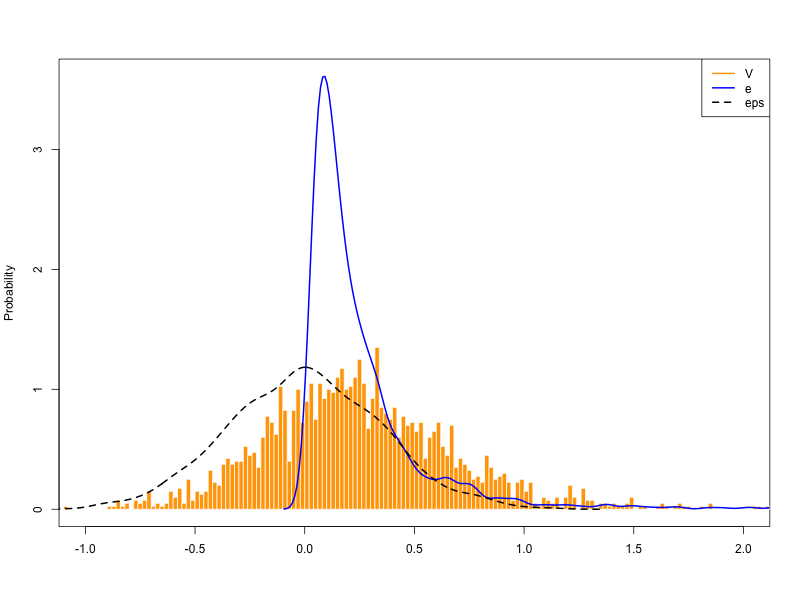
\includegraphics{../Code/Products/bs_mle_hist.png}

}

\caption{\label{fig-simulated-data}Simulated data}

\end{figure}%

I then used the logspline model to estimate the parameters of the
distribution of \(e\). I used a B-spline basis with 10 knots. The knots
where placed at equally spaced percentiles of the non-negative \(V\)
observations. For the integral, I used Gauss Legendre quadrature. To
ensure good coverage of the high probability region of the density, I
used a recursive function to form a grid placing a higher number of
nodes in the high probability region. I set the penalty parameter
\(\lambda\) to 0.1. The estimated density is shown in
Figure~\ref{fig-simulated-deconv}.

\begin{figure}

\centering{

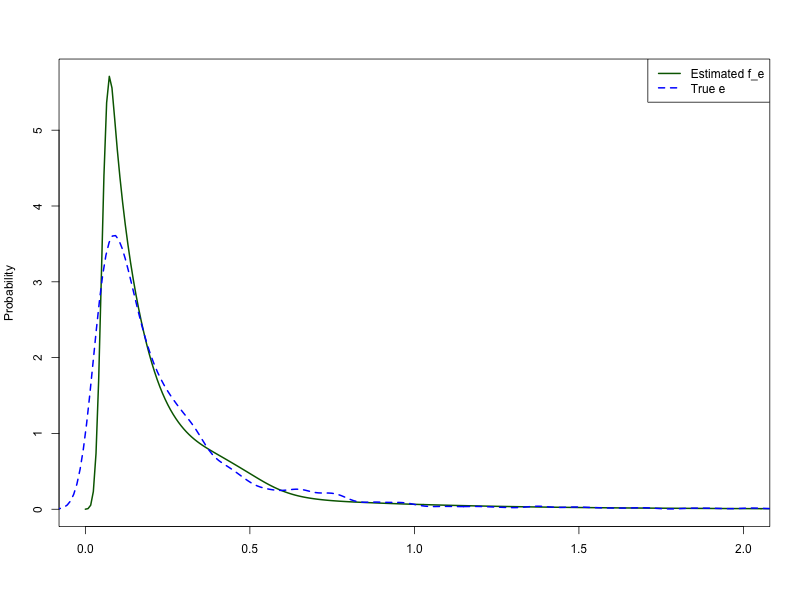
\includegraphics{../Code/Products/bs_mle.png}

}

\caption{\label{fig-simulated-deconv}LogSpline Deconvolution}

\end{figure}%

\section{Results}\label{results}

\subsection{Testing for the Presence of Tax Evasion Through
Overreporting}\label{sec-tax-ev-test}

Equation~\ref{eq-ob-ev} suggest a way to test the presence of tax
evasion through cost overreporting. Let
\(\mathbb{E}[\mathcal{V}_{it}]\equiv \mu_{\mathcal{V}}\). Define the
null hypothesis as the absence of cost overreporting,
\(H_0: \mu_{\mathcal{V}}=0\), and the alternative hypothesis as the
presence of cost overreporting, \(H_1: \mu_{\mathcal{V}}>0\).
Consequently, we can use a one-sided t-test to verify for the presence
of tax evasion by overreporting.

Under the null hypothesis, there is no tax evasion. Then, \[
\begin{aligned}  
  z &= \frac{\bar{\mathcal{V}}}{\hat\sigma_{\mathcal{V}}/\sqrt{N}}=\frac{\mathbb{E}[\mathcal{V}]}{\sqrt{\mathbb{Var}[\mathcal{V}]/N}}\\
  &=\frac{-\mathbb{E}[\varepsilon]+\mathbb{E}[e]}{\sqrt{\mathbb{Var}[\varepsilon]+\mathbb{Var}[e]/N}}\\
  &= \frac{-\mathbb{E}[\varepsilon]}{\sqrt{\mathbb{Var}[\varepsilon]/N}}\sim N(0,1)
\end{aligned}
\]

The previous test ignores the sample variance of the \(\beta\) estimator
in the first stage.

Alternatively, we can do a difference in means test to account for this
variation. This test is equivalent to a two sample GMM test, where in
one moment the corporations are used to estimate \(\hat\beta\) and the
second is a test moment where we use \(\hat\beta\) from the first one.
Under the null, the two moment should be equal to zero.

Let \(s_{it}=log\left(\frac{\rho_t M^*_{it}}{P_t Y_{it}}\right)\) and
\(\bar s_G= \frac{1}{N_1T_1}\sum_{i=1}^{N_1}\sum_{t=1}^{T_1}s_{it}^G\)
and
\(\bar s_B= \frac{1}{N_2T_2}\sum_{i=1}^{N_2}\sum_{t=1}^{T_2}s_{it}^B\)
be the sample means for good guys (corporations) and the tax evasion
guys, respectively.

Then, the test statistic is,

\[
\begin{aligned}  
  t &= \frac{\bar s_B - \bar s_G}{\sqrt{\hat\sigma^2_{\bar s_B}/N_2T_2 + \hat\sigma^2_{\bar s_G}/N_1T_1}} \sim N(0,1) \text{ under } H_0\\
\end{aligned}
\]

where \(\hat\sigma^2_{\bar s_B}\) and \(\hat\sigma^2_{\bar s_G}\) are
the sample variances of \(s_{it}^B\) and \(s_{it}^G\), respectively.

Of course, the assumption of independent samples is likely incorrect.
For example, firms in an industry might get contemporaneous shocks
affecting everyone in one period, like a price shock in inputs.
Productivity is usually assumed to be persistent over time, but the
effects of productivity of one firm on the other firms is commonly
ignored. In addition, if the data uses SIC codes, firms within
sub-industries are more likely to be correlated than firms in different
sub-industries.

I test for the presence of tax evasion for different classifications of
intermediates. Intermediates include raw materials, energy and services.
Deductibles include raw materials and deductible expenses. Materials
include only raw materials. The items included as deductible expenses or
services are detailed in \textbf{?@tbl-expenses-type}

\begin{table}

\caption{\label{tbl-evasion-test-CD}Tax Evasion Through
Cost-Overreporting One-Side t-Test by Industry in Colombia. Under the
null hypothesis, there is no tax evasion. Values of the statistic were
computed from Equation~\ref{eq-ob-ev} for different intermediate inputs.
Standard errors shown in parethesis. Stars indicate significance level
at the 1\% (***), 5\% (**), and 10\% (*).}

\centering{

\centering
\begin{tabular}[t]{r|l|l|l|l|l|l}
\hline
SIC & Category & Deductibles & Materials & Electricity & Fuels & R\&M\\
\hline
311 & 1 Exempt Product & 0.0294 (0.005)*** & 0.1111 (0.0045)*** & 2.1331 (0.0201)*** & 2.7032 (0.0234)*** & 2.989 (0.0348)***\\
\cline{1-7}
312 & 1 Exempt Product & 0.0251 (0.0115)** & -0.0098 (0.0158) & 3.2172 (0.0702)*** & 3.4251 (0.0559)*** & 3.4931 (0.0698)***\\
\cline{1-7}
383 & 1 Exempt Product & 0.056 (0.0101)*** & 0.0471 (0.0108)*** & 2.3743 (0.1024)*** & 3.7437 (0.0916)*** & 2.9996 (0.0326)***\\
\cline{1-7}
322 & 4 Direct Customer Sales & 0.6404 (0.0068)*** & 1.27 (0.0068)*** & 2.1725 (0.068)*** & 3.7666 (0.1205)*** & 2.9369 (0.04)***\\
\cline{1-7}
342 & 4 Direct Customer Sales & 0.0711 (0.0077)*** & 0.0936 (0.0082)*** & 2.2239 (0.0814)*** & 3.3124 (0.0918)*** & 2.1927 (0.0468)***\\
\cline{1-7}
390 & 4 Direct Customer Sales & 0.0866 (0.0124)*** & 0.0761 (0.0131)*** & 2.2658 (0.0478)*** & 3.8163 (0.1293)*** & 3.3716 (0.1142)***\\
\cline{1-7}
321 &  & 0.0885 (0.007)*** & 0.1262 (0.0078)*** & 1.4567 (0.0255)*** & 2.77 (0.0286)*** & 3.1702 (0.1098)***\\
\cline{1-7}
313 &  & 0.0377 (0.0111)*** & 0.0659 (0.0123)*** & 1.7785 (0.0315)*** & 2.0103 (0.0428)*** & 2.2176 (0.0881)***\\
\cline{1-7}
351 &  & 0.0171 (0.0145) & 0.1116 (0.0221)*** & 1.6454 (0.0406)*** & 2.7385 (0.0444)*** & 2.2409 (0.0539)***\\
\cline{1-7}
352 &  & 0.0462 (0.0079)*** & 0.0414 (0.0083)*** & 2.8723 (0.0918)*** & 3.8478 (0.107)*** & 3.0485 (0.047)***\\
\hline
\end{tabular}

}

\end{table}%

\begin{table}

\caption{\label{tbl-tax-ev-test-context}Tax Evasion Through
Cost-Overreporting One-Side t-Test by Industry in Colombia. Under the
null hypothesis, there is no tax evasion. Values of the statistic were
computed from Equation~\ref{eq-ob-ev}. Standard errors shown in
parethesis. Stars indicate significance level at the 1\% (***), 5\%
(**), and 10\% (*).}

\centering{

\centering
\begin{tabular}[t]{r|r|r|r|r|r|r|r|r|r|r|r|r|r|l|l}
\hline
sic\_3 & n & n\_Corp & share\_sales\_tax & gross\_output & sales & deductible\_intermediates & materials & share\_exports & share\_imports & share\_imports\_materials & importers & exporters & importers\_mats & log\_mats\_share & log\_deductible\_intermediates\_share\\
\hline
311 & 888 & 147 & 0.0 & 0.2 & 0.2 & 0.3 & 0.3 & 0.0 & 0.0 & 0.1 & 0.1 & 0.1 & 0.2 & 0.1111 (0.0045)*** & 0.0294 (0.005)***\\
\cline{1-16}
312 & 188 & 41 & 0.0 & 0.0 & 0.1 & 0.1 & 0.1 & 0.0 & 0.1 & 0.1 & 0.3 & 0.1 & 0.3 & -0.0098 (0.0158) & 0.0251 (0.0115)**\\
\cline{1-16}
313 & 130 & 74 & 0.1 & 0.1 & 0.1 & 0.1 & 0.1 & 0.0 & 0.0 & 0.1 & 0.3 & 0.0 & 0.4 & 0.0659 (0.0123)*** & 0.0377 (0.0111)***\\
\cline{1-16}
321 & 470 & 71 & 0.1 & 0.1 & 0.1 & 0.1 & 0.1 & 0.0 & 0.1 & 0.1 & 0.3 & 0.2 & 0.3 & 0.1262 (0.0078)*** & 0.0885 (0.007)***\\
\cline{1-16}
322 & 737 & 22 & 0.1 & 0.0 & 0.0 & 0.0 & 0.0 & 0.0 & 0.0 & 0.0 & 0.1 & 0.1 & 0.1 & 1.27 (0.0068)*** & 0.6404 (0.0068)***\\
\cline{1-16}
323 & 99 & 13 & 0.1 & 0.0 & 0.0 & 0.0 & 0.0 & 0.2 & 0.0 & 0.0 & 0.3 & 0.4 & 0.4 & -0.1534 (0.0133) & -0.1635 (0.0137)\\
\cline{1-16}
324 & 192 & 9 & 0.1 & 0.0 & 0.0 & 0.0 & 0.0 & 0.0 & 0.0 & 0.0 & 0.1 & 0.2 & 0.2 & 0.0664 (0.0086)*** & 0.0578 (0.0084)***\\
\cline{1-16}
331 & 172 & 13 & 0.1 & 0.0 & 0.0 & 0.0 & 0.0 & 0.0 & 0.0 & 0.0 & 0.1 & 0.1 & 0.1 & 0.2177 (0.0154)*** & 0.1205 (0.0139)***\\
\cline{1-16}
332 & 193 & 12 & 0.1 & 0.0 & 0.0 & 0.0 & 0.0 & 0.0 & 0.0 & 0.0 & 0.1 & 0.0 & 0.1 & -0.028 (0.0136) & -0.0284 (0.0127)\\
\cline{1-16}
341 & 153 & 41 & 0.1 & 0.1 & 0.1 & 0.1 & 0.1 & 0.0 & 0.1 & 0.1 & 0.2 & 0.2 & 0.3 & -0.0067 (0.0112) & -0.0284 (0.0094)\\
\cline{1-16}
342 & 347 & 40 & 0.1 & 0.0 & 0.0 & 0.0 & 0.0 & 0.0 & 0.1 & 0.1 & 0.2 & 0.1 & 0.3 & 0.0936 (0.0082)*** & 0.0711 (0.0077)***\\
\cline{1-16}
351 & 116 & 68 & 0.1 & 0.1 & 0.1 & 0.1 & 0.1 & 0.1 & 0.3 & 0.2 & 0.6 & 0.4 & 0.6 & 0.1116 (0.0221)*** & 0.0171 (0.0145)\\
\cline{1-16}
352 & 300 & 100 & 0.1 & 0.1 & 0.1 & 0.1 & 0.1 & 0.0 & 0.2 & 0.3 & 0.6 & 0.3 & 0.7 & 0.0414 (0.0083)*** & 0.0462 (0.0079)***\\
\cline{1-16}
356 & 272 & 53 & 0.1 & 0.0 & 0.0 & 0.0 & 0.0 & 0.0 & 0.1 & 0.2 & 0.4 & 0.2 & 0.5 & -0.077 (0.0084) & -0.0517 (0.0073)\\
\cline{1-16}
369 & 274 & 58 & 0.1 & 0.0 & 0.0 & 0.0 & 0.0 & 0.0 & 0.1 & 0.1 & 0.2 & 0.1 & 0.2 & 0.5516 (0.0161)*** & -0.0237 (0.0105)\\
\cline{1-16}
381 & 633 & 85 & 0.1 & 0.0 & 0.0 & 0.0 & 0.0 & 0.0 & 0.1 & 0.2 & 0.3 & 0.2 & 0.4 & -0.0014 (0.0065) & 3e-04 (0.0058)\\
\cline{1-16}
382 & 364 & 46 & 0.1 & 0.0 & 0.0 & 0.0 & 0.0 & 0.0 & 0.1 & 0.2 & 0.3 & 0.2 & 0.5 & -0.0022 (0.0087) & 0.0095 (0.0077)\\
\cline{1-16}
383 & 213 & 57 & 0.1 & 0.0 & 0.0 & 0.0 & 0.0 & 0.0 & 0.3 & 0.3 & 0.6 & 0.2 & 0.7 & 0.0471 (0.0108)*** & 0.056 (0.0101)***\\
\cline{1-16}
384 & 238 & 42 & 0.1 & 0.1 & 0.1 & 0.1 & 0.1 & 0.0 & 0.2 & 0.2 & 0.4 & 0.2 & 0.5 & -0.0924 (0.0118) & -0.0824 (0.0101)\\
\cline{1-16}
390 & 179 & 18 & 0.1 & 0.0 & 0.0 & 0.0 & 0.0 & 0.0 & 0.1 & 0.2 & 0.4 & 0.3 & 0.5 & 0.0761 (0.0131)*** & 0.0866 (0.0124)***\\
\hline
\end{tabular}

}

\end{table}%

Table~\ref{tbl-evasion-test-CD} shows that the null hypothesis of no tax
evasion is rejected at the 1\% significance level for twelve of the top
twenty manufacturing industries.

In particular, there is no evidence of tax evasion for most industries
in which products or raw materials are exempt of sales taxes, such as
312 (Other Food Products), 382 (Non-Electrical Machinery), 384
(Transport Equipment), 323 (Leather Products), and 369 (Non-Metallic
Mineral Products); there is also no evidence of materials overreporting
for 356 (Plastic Products)industry, whose main raw materials are likely
to be specialized and supplied by few local and international suppliers.

Among the industries with exempted products, 311 (Food Products) and 383
(Electrical Machinery) there is evidence of tax evasion but as we'll see
later the average overreporting is low compared to other industries.

As expected, the evidence is stronger particularly for the other
industries that do not fall in the previous categories. Namely, there is
evidence of tax evasion for industries 313 (Beverages); for 321
(Textiles), 322 (Wearing Apparel), and 324 (Footwear); 331 (Wood
Products except Furniture) and 332 (Wood Furniture); for industry 341
(Paper) and 342 (Publishing); 351 (Industrial Chemicals) and 352 (Other
Chemicals); 381 (Metal Products Except Machinery), and 390 (Other
Manufacturing Industries).

\subsection{Deconvoluting Tax Evasion Using
Moments}\label{deconvoluting-tax-evasion-using-moments}

One simple way to start with the deconvolution is using moments. In
particular, for every \(n\)-th moment
\(\mathbb{E}[\varepsilon_{it}^n|\Theta^{NE}]=\mathbb{E}[\varepsilon_{it}^n|t]=\mathbb{E}[\varepsilon_{it}^n]\)

Therefore, any moment of the tax evasion \(e_{it}\) distribution
\(\forall t\in T\) can be estimated in theory.

Namely, from Equation~\ref{eq-ob-ev}, we can estimate the average tax
evasion by \[
\begin{aligned}
  \mathbb{E}[e_{it}|t]&=\mathbb{E}[\mathcal V_{it}|t]+\mathbb{E}[\varepsilon_{it}]\\
  &=\mathbb{E}[\mathcal V_{it}|t]+\mu_{\varepsilon}
  % \\
  % \mathbb{V}[e_{it}|t]&=\mathbb{V}[\mathcal V_{it}|t]-\mathbb{V}[\varepsilon_{it}]\\
  % &=\mathbb{V}[\mathcal V_{it}|t]-\sigma^2_{\varepsilon}
\end{aligned}
\]

Note that we learned the distribution \(f_\varepsilon(\varepsilon)\) of
\(\varepsilon\) from the first stage, so \(\mu_{\varepsilon}\) and
\(\sigma_{\varepsilon}\) are known.

Table~\ref{tbl-tax-ev-deconv-moments} displays the estimated average of
the log fraction that firms increase their costs of raw materials to
evade taxes by claiming a greater deductible amount of their owed sales
taxes.

\begin{table}

\caption{\label{tbl-tax-ev-deconv-moments}Average tax evasion by
Industry. Estimates show the average tax evasion from the output shock
in Equation~\ref{eq-ob-ev}. LCI and UCI are the bias-corrected bootsrap
confidence intervals at the 10\% significance level with 250 bootstrap
replicates. Intermediates are defined as raw materials.}

\centering{

\centering
\begin{tabular}[t]{l|l|r|r|r}
\hline
SIC & Inter & Mean & LCI & UCI\\
\hline
331 & Materials & 0.2177 & 0.0973 & 0.3764\\
\cline{1-5}
322 & Materials & 0.1955 & 0.1007 & 0.3007\\
\cline{1-5}
369 & Materials & 0.1446 & 0.0580 & 0.2702\\
\cline{1-5}
313 & Materials & 0.0659 & 0.0312 & 0.1091\\
\cline{1-5}
321 & Materials & 0.1094 & 0.0793 & 0.1793\\
\hline
\end{tabular}

}

\end{table}%

The top five tax evading industries, 322 (Wearing Apparel), 342
(Publishing), 313 (Beverages), 351 (Industrial Chemicals), and 331 (Wood
Products), display an average tax evasion \(e\) greater than 12\%, which
is non-trivial.

Although deconvolution by moments is the simplest method, it displays
the undesirable characteristic that estimate of variances frequently
result with a negative sign. In the next section, I address this problem
by using parametric MLE.

\subsection{Deconvoluting by Parametric
MLE}\label{deconvoluting-by-parametric-mle}

I use parametric MLE to obtain better estimates of the variances using
equation Equation~\ref{eq-mle}. I assume that the error term
\(\varepsilon\) follows a normal distribution.

For tax-evasion, theory suggests that firms only have incentives to
overreport costs, not to underreport them. Therefore, as explained
elsewhere, it might be expected that overreporting \(e\ge0\) is
non-negative. In addition, it might also be expected that most firms
overreport a little and a few firms overreport greater amounts.
Therefore, a lognormal or a truncated normal distribution might be more
appropriate.

By definition, if a random variable \(U\) is log-normal distributed,
then \(log(U)\sim N(\mu, \sigma)\). Thus, we cannot directly compare the
parameters of the log-normal distribution to our previous estimates. We
can however, used the parameters to compute any moment of the
log-normally distributed variable \(U\) by

\[
E[U^n]=e^{n\mu+\frac{1}{2}n^2\sigma^2}
\]

In particular, the first moment and the variance are computed as
follows,

\[
\begin{aligned}  
E[U]&=e^{\mu+\frac{1}{2}\sigma^2}\\
Var[U]&=E[U^2]-E[U]^2=e^{2\mu+\sigma^2}(e^{\sigma^2}-1).
\end{aligned}
\]

In addition, the mode and the mean by

\[
\begin{aligned}
  \text{Mode}[U]&=e^{\mu-\sigma^2} \\
  \text{Med}[U]&=e^{\mu}
\end{aligned}
\]

Likewise, the probability density function of random variable \(U\) with
a normal distribution with parameters \(\tilde\mu\) and \(\tilde\sigma\)
and truncated from below at zero is

\[
  f(u\\;\tilde\mu,\tilde\sigma) = \frac{\varphi(\frac{u-\tilde\mu}{\tilde\sigma})}{\tilde\sigma (1-\Phi(\alpha))}
\]

where

\[
\varphi(\xi)=\frac{1}{2\pi}\exp(-\frac{1}{2}\xi^2)
\]

is the probability density function of the standard normal distribution,
\(\Phi(\centerdot)\) is its cumulative distribution function, and
\(\alpha=-\tilde\mu/\tilde\sigma\)

Then, the mean becomes

\[
E[U|U>0]=\tilde\mu+\tilde\sigma\frac{\varphi(\alpha)}{1-\Phi(\alpha)}
\]

and the variance, median, and mode become

\[
\begin{aligned}  
Var[U|U>0]&=\sigma^2[1+\alpha\varphi(\alpha)/(1-\Phi(\alpha))-(\varphi(\alpha)/[1-\Phi(\alpha)])^2]\\
\text{Median}[U|U>0]&=\tilde\mu+\Phi^{-1}\left(\frac{\Phi(\alpha)+1}{2}\right)\tilde\sigma \\ 
\text{Mode}[U|U>0]&=\tilde\mu
\end{aligned}
\]

Table~\ref{tbl-deconv-mle-both} displays the estimates of the parameters
for both the log-normal and truncated normal distributions using an MLE
approach. Other moments of the densities are computed as explained
previously and shown for reference.

\begin{longtable}[t]{llrrrrrr}

\caption{\label{tbl-deconv-mle-both}Estimates of Deconvoluting Tax
Evasion from the Output Shock in Equation~\ref{eq-ob-ev} by Parametric
MLE Using A Log-Normal and a Truncated-Normal Distribution. \(\mu\) and
\(\sigma\) are the parameters of the densities. Moments displayed are
estimated using the distribution paramters as explained above.
Intermediates are defined as raw materials.}

\tabularnewline

\toprule
sic\_3 & dist & mu & sigma & mean & sd & mode & median\\
\midrule
 & lognormal & -1.7460 & 0.9181 & 0.2659 & 0.3059 & 0.0751 & 0.1745\\
\cmidrule{2-8}\nopagebreak
\multirow[t]{-2}{*}{\raggedright\arraybackslash 311} & truncated normal & 0.2280 & 0.0894 & 0.2294 & 0.0876 & 0.2280 & 0.2286\\
\cmidrule{1-8}\pagebreak[0]
 & lognormal & -1.4006 & 0.9855 & 0.4005 & 0.5131 & 0.0933 & 0.2465\\
\cmidrule{2-8}\nopagebreak
\multirow[t]{-2}{*}{\raggedright\arraybackslash 313} & truncated normal & 0.3285 & 0.1647 & 0.3376 & 0.1549 & 0.3285 & 0.3332\\
\cmidrule{1-8}\pagebreak[0]
 & lognormal & -1.4011 & 0.8883 & 0.3655 & 0.4006 & 0.1119 & 0.2463\\
\cmidrule{2-8}\nopagebreak
\multirow[t]{-2}{*}{\raggedright\arraybackslash 321} & truncated normal & 0.3183 & 0.1302 & 0.3209 & 0.1269 & 0.3183 & 0.3195\\
\cmidrule{1-8}\pagebreak[0]
 & lognormal & -1.5406 & 0.9517 & 0.3370 & 0.4091 & 0.0866 & 0.2143\\
\cmidrule{2-8}\nopagebreak
\multirow[t]{-2}{*}{\raggedright\arraybackslash 352} & truncated normal & 0.2847 & 0.1218 & 0.2879 & 0.1180 & 0.2847 & 0.2862\\
\cmidrule{1-8}\pagebreak[0]
 & lognormal & -1.5748 & 0.9288 & 0.3187 & 0.3730 & 0.0874 & 0.2071\\
\cmidrule{2-8}\nopagebreak
\multirow[t]{-2}{*}{\raggedright\arraybackslash 383} & truncated normal & 0.2718 & 0.1230 & 0.2761 & 0.1180 & 0.2718 & 0.2739\\
\bottomrule

\end{longtable}

Both the log-normal and the truncated normal distributions point to
similar means. The differences between the other moments of the
distributions can be explained by the differences in the shapes of their
probability density functions. The standard deviation is larger in the
log-normal distribution than in the truncated normal distribution which
can be explained by the asymmetry of the log normal distribution which
is skewed to the right. With respect to the mode, it is the same to the
mean in the case of the truncated normal distribution, while it is lower
than the median for the log-normal. Finally, the median is lower than
the mean in the case of the log-normal, but higher than the mean in the
case of the truncated normal because of the truncation from below.

Both distributions show higher estimates of the average overreporting in
logs than using only moments. Now it looks like firms evade taxes by
inflating their cost of their materials by 40 percent or more.

Table~\ref{tbl-deconv-mle-boot} shows the bias corrected bootstrap
confidence intervals for the mean of each distribution by industry using
200 replicates.

\begin{longtable}[t]{llll}

\caption{\label{tbl-deconv-mle-boot}Estimates of Deconvoluting Tax
Evasion from the Output Shock in Equation~\ref{eq-ob-ev} by Parametric
MLE Using A Log-Normal and a Truncated-Normal Distribution. LCI and UCI
are the bias corrected bootstrap confidence intervals at the 5 percent
significance level using 250 replicates.}

\tabularnewline

\toprule
SIC & Density & Mean & SD\\
\midrule
 &  & 0.2659 & 0.3059\\
\cmidrule{3-4}\nopagebreak
 & \multirow[t]{-2}{*}{\raggedright\arraybackslash lognormal} & {}[0.2285, 0.2999] & {}[0.2069, 0.3536]\\
\cmidrule{2-4}\nopagebreak
 &  & 0.2294 & 0.0876\\
\cmidrule{3-4}\nopagebreak
\multirow[t]{-4}{*}[1\dimexpr\aboverulesep+\belowrulesep+\cmidrulewidth]{\raggedright\arraybackslash 311} & \multirow[t]{-2}{*}{\raggedright\arraybackslash truncated normal} & {}[0.2116, 0.2597] & {}[0.0791, 0.0991]\\
\cmidrule{1-4}\pagebreak[0]
 &  & 0.4005 & 0.5131\\
\cmidrule{3-4}\nopagebreak
 & \multirow[t]{-2}{*}{\raggedright\arraybackslash lognormal} & {}[0.3407, 0.468] & {}[0.3279, 0.6767]\\
\cmidrule{2-4}\nopagebreak
 &  & 0.3376 & 0.1549\\
\cmidrule{3-4}\nopagebreak
\multirow[t]{-4}{*}[1\dimexpr\aboverulesep+\belowrulesep+\cmidrulewidth]{\raggedright\arraybackslash 313} & \multirow[t]{-2}{*}{\raggedright\arraybackslash truncated normal} & {}[0.2965, 0.3831] & {}[0.1343, 0.1791]\\
\cmidrule{1-4}\pagebreak[0]
 &  & 0.337 & 0.4091\\
\cmidrule{3-4}\nopagebreak
 & \multirow[t]{-2}{*}{\raggedright\arraybackslash lognormal} & {}[0.2718, 0.3804] & {}[0.2442, 0.4747]\\
\cmidrule{2-4}\nopagebreak
 &  & 0.2879 & 0.118\\
\cmidrule{3-4}\nopagebreak
\multirow[t]{-4}{*}[1\dimexpr\aboverulesep+\belowrulesep+\cmidrulewidth]{\raggedright\arraybackslash 352} & \multirow[t]{-2}{*}{\raggedright\arraybackslash truncated normal} & {}[0.2509, 0.3287] & {}[0.1046, 0.134]\\
\cmidrule{1-4}\pagebreak[0]
 &  & 0.3655 & 0.4006\\
\cmidrule{3-4}\nopagebreak
 & \multirow[t]{-2}{*}{\raggedright\arraybackslash lognormal} & {}[0.3176, 0.4179] & {}[0.2702, 0.4448]\\
\cmidrule{2-4}\nopagebreak
 &  & 0.3209 & 0.1269\\
\cmidrule{3-4}\nopagebreak
\multirow[t]{-4}{*}[1\dimexpr\aboverulesep+\belowrulesep+\cmidrulewidth]{\raggedright\arraybackslash 321} & \multirow[t]{-2}{*}{\raggedright\arraybackslash truncated normal} & {}[0.2909, 0.3751] & {}[0.1183, 0.1443]\\
\cmidrule{1-4}\pagebreak[0]
 &  & 0.3187 & 0.373\\
\cmidrule{3-4}\nopagebreak
 & \multirow[t]{-2}{*}{\raggedright\arraybackslash lognormal} & {}[0.2613, 0.3727] & {}[0.2391, 0.4416]\\
\cmidrule{2-4}\nopagebreak
 &  & 0.2761 & 0.118\\
\cmidrule{3-4}\nopagebreak
\multirow[t]{-4}{*}[1\dimexpr\aboverulesep+\belowrulesep+\cmidrulewidth]{\raggedright\arraybackslash 383} & \multirow[t]{-2}{*}{\raggedright\arraybackslash truncated normal} & {}[0.226, 0.3368] & {}[0.1082, 0.1351]\\
\bottomrule

\end{longtable}

The difference between our previous estimates using moments can be
explained by the fact that the log-normal and truncated distribution are
restricted to positive values while we did not apply the restriction
when using moments. Were we to take the average of only the positive
values, the mean of the moments' method would be higher and closer to
the log-normal and truncated normal distributions.

From the perspective of theory, firms would have incentives to
overreport their materials. Therefore, using moments to estimate
overreporting without restricting to positive values like in the case of
the MLE method using a log-normal or truncated distribution might
underestimate tax evasion through cost overreporting.

\begin{figure}

\begin{minipage}{\linewidth}

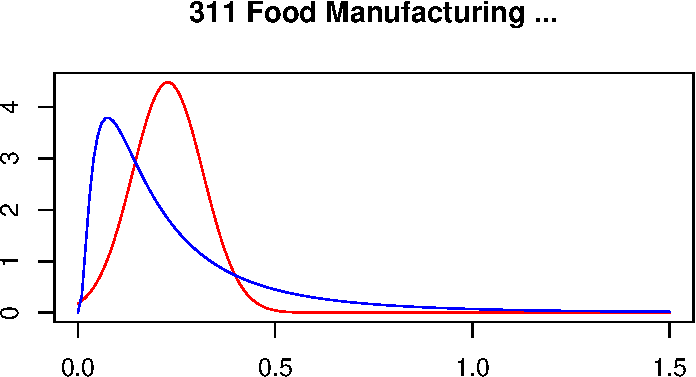
\includegraphics{Tax-Prod_files/figure-pdf/unnamed-chunk-13-1.pdf}

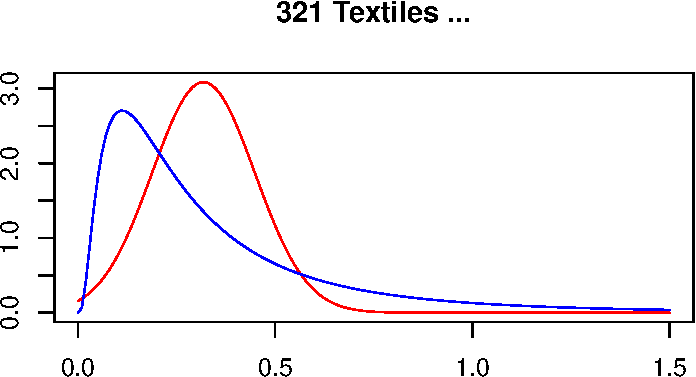
\includegraphics{Tax-Prod_files/figure-pdf/unnamed-chunk-13-2.pdf}

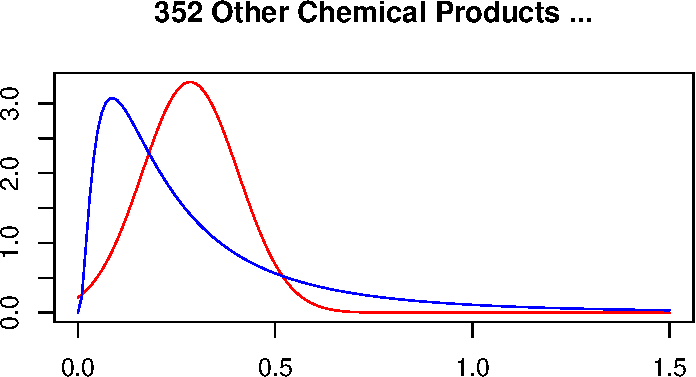
\includegraphics{Tax-Prod_files/figure-pdf/unnamed-chunk-13-3.pdf}

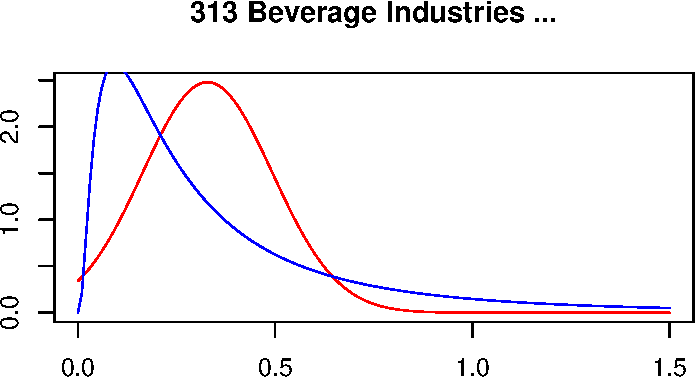
\includegraphics{Tax-Prod_files/figure-pdf/unnamed-chunk-13-4.pdf}

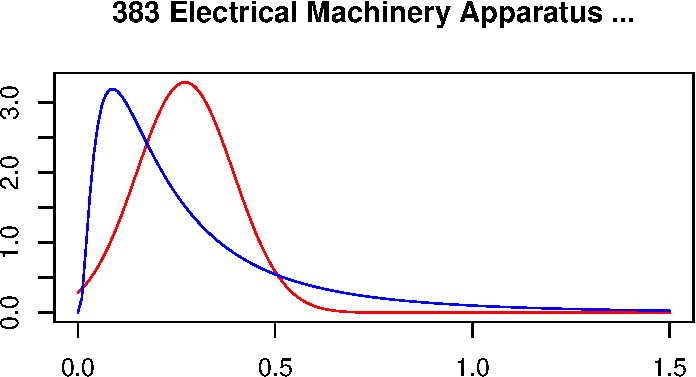
\includegraphics{Tax-Prod_files/figure-pdf/unnamed-chunk-13-5.pdf}

\begin{verbatim}
NULL
NULL
NULL
NULL
NULL
\end{verbatim}

\end{minipage}%

\caption{\label{fig-density-plots}Truncated Normal (red) and Log-Normal
(blue) distribution of the overreporting of raw materials for the top
tax-evading industries.}

\end{figure}%

\subsection{Non-Parametric Deconvolution using Penalized
B-Splines}\label{non-parametric-deconvolution-using-penalized-b-splines}

\begin{table}

\caption{\label{tbl-np-deconv}Semiparametric Deconvolution of Tax
Evasion using Penalized B-Splines. I used a kernel density estimator to
fit the error density on the residuals of the first stage conditional on
firms being Non-Evaders.}

\centering{

\centering
\begin{tabular}[t]{l|r|r|r}
\hline
sic\_3 & mean & sd & skewness\\
\hline
331 & 0.191 & 0.080 & 0.782\\
\hline
322 & 0.185 & 0.037 & 0.117\\
\hline
369 & 0.077 & 0.027 & 22.485\\
\hline
313 & 0.077 & 0.096 & 7.320\\
\hline
321 & 0.127 & 0.044 & 0.566\\
\hline
\end{tabular}

}

\end{table}%

\section{Getting the Story Straight}\label{getting-the-story-straight}

Firms face incentives to evade sales taxes by overreporting their input
costs. Firms overreport their cost by acquiring fake invoices to claim
additional deductions of their sales taxes, maximizing after-tax
profits. The higher the sales tax, the greater the incentive to evade.
However, the probability of detection and the threat of penalties limit
how much firms overreport.

The key incentive for firms is the \textbf{effective sales tax rate} ---
the amount firms ultimately pay or receive from the tax authority. The
effective tax rate is calculated as the difference between the total
sales tax charged by the firm on its sales and the total sales tax paid
by the firm on its inputs, divided by total sales. A positive difference
indicates what the firm should pay to the government. If the difference
is negative, the firm receives a refund from the tax authority.

\[
\begin{aligned}
\tau &= \frac{\tau_0P_tY_{it} - \tau_1\rho_t M_{it}}{P_tY_{it}} \\
&= \tau_0 - \tau_1 \beta
\end{aligned}
\]

In Colombia, the total amount charged by the firm as sales tax depends
on the statutory tax rate of each product sold domestically;
\textbf{exports are exempt} from sales tax. Low statutory sales tax
rates and exempt products result in lower sales tax collected by the
firm and thus, a lower effective tax rate. Consequently, firms whose
products are exempt from sales tax or taxed with \textbf{low statutory
rates} have low incentives to evade. Likewise, as the share of their
exports increases, exporter firms bear decreasing incentives to evade
taxes because a larger portion of their sales is exempt from sales tax,
reducing the effective sales tax rate.

On the other hand, the total amount paid by the firm as sales tax
depends on the statutory tax rate of each of its inputs, including
imports. \textbf{Imports}, in contrast to exports, are \textbf{not
exempt}. Hence, the composition of the foreign and domestic inputs does
not affect the effective sales tax rate, nor the incentives to evade.
However, the tax system imposed a zero sales tax rate on
\textbf{unprocessed primary inputs}, such as forestry, mining, fishing,
and agriculture. Therefore, firms consuming a high share of primary
inputs face a higher effective sales tax rate and thus, greater
incentives to evade.

Note that the effective sales tax rate might naturally be
\textbf{negative} for firms in certain industries. Before the 1983
reform in Colombia, there were four different statutory sales tax rates:
4, 10, 15 and 25 percent. Because the sales tax was applied at the
product level, \emph{the total amount paid as sales tax by the firms on
its inputs could be larger than the total amount charged by the firm as
sales tax on its products.} This situation would result in a negative
effective sales tax rate. Firms in this situation would receive a refund
from the tax authority.

Would firms with negative effective tax rates have incentives to
overreport inputs to increase their refunds? Unlikely. Although the
refunds had to be made within 30 days, \emph{the procedure was
complicated, and the tax authority delayed, on average, one year to
process the payment}. Suspicion of fraudulent activities might further
delay the process. Therefore, firms in this situation did not have
incentives to overreport inputs to increase their refunds.

Whether firms in certain industries have incentives to overreport their
inputs to evade sales taxes might \textbf{not} be \textbf{obvious}
\emph{ex-ante}. The tax code might be complex, with many exemptions and
different statutory rates. Different taxes might generate overlapping or
conflicting incentives. Available data might lack details on the
products or inputs used by firms, making it difficult to identify the
effective sales tax rate.

A first contribution of this paper is to provide practitioners and
policymakers a way to identify industries where tax evasion through
cost-overreporting might be non-trivial and can be identified from data.
The simple model employed in this paper to investigate the mechanisms of
tax evasion provides conditions that can be tested with data. As a
result, I propose a statistical test where the null hypothesis states
that firms in an industry of interest do not evade sales taxes by
overreporting; the alternative states that firms do commit tax evasion
Section~\ref{sec-tax-ev-test}.

Failing to reject the null hypothesis does not necessarily imply that
firms in this industry are not overreporting. If a researcher suspects
this practcie on a particular industry, he would have to investigate if
the assumptions of the model are not unreasonable for said industry. The
main assumption comes from the production function method, even though
they might differ in their productivity, evaders and non-evaders share a
common technology.

With this in mind, in any dataset using SIC codes, it should be
considered that the SIC codes groups firms with similar products, but
some categories might group products that require different
technologies. Furthermore, most firms are multiproducts, and might be
classified under a certain SIC code because it produces more of a
certain product marginally.

\subsection{Showing the Evidence}\label{showing-the-evidence}

\begin{table}

\caption{\label{tbl-ielas-top5}Intermediate elasticities for
Corporations (Non-Evaders) and non-Corporations (Evaders) for different
industries. Estimates were obtained using GNR (2020) method assuming a
CD functional form. Intermediates are defined as raw materials.
\(\varepsilon\) is defined as \textbf{measurement error}. The Tax
Evasion Test displays the coefficient of the statistical test, where the
null hypothesis states that there is no tax evasion through cost
overreporting. Among the industry characteristics, Sales is the
industry's market share of the total sales in Colombia between 1981 and
1991. Sales Tax Rate is the average sales tax reported rate. Exports is
the average share of exports of the industry total sales, and Exporters
is the share of firms exporting 10 percent or more of their total sales.
Bias-corrected bootstrap confidence intervals at 95\% significanve level
are displayed in brackets. *, **, *** denote significance at the 10\%,
5\%, and 1\% levels (one-sided).}

\centering{

\centering
\begin{tabular}[t]{c|c|c|c|c|c|c|c|c|c}
\hline
\multicolumn{1}{c|}{ } & \multicolumn{2}{c|}{Elasticities} & \multicolumn{1}{c|}{Test} & \multicolumn{3}{c|}{ } & \multicolumn{3}{c}{Sales Tax Rate} \\
\cline{2-3} \cline{4-4} \cline{8-10}
SIC & Corps. & Others & Tax Ev. & N & N (Corps.) & Sales (Mkt \%) & Effective & Sales & Purchases\\
\hline
 & 0.6 & 0.61 & 0.02* & 888 & 147 & 23.6 & -0.1 & 0.2 & 0.5\\
\cline{2-10}
\multirow[t]{-2}{*}{\centering\arraybackslash 311} & [0.57, 0.62] & [0.59, 0.62] & [-0.02, 0.08] &  &  &  &  &  & \\
\cline{1-10}
 & 0.29 & 0.35 & 0.18*** & 130 & 74 & 9.7 & 7.7 & 8.4 & 2.3\\
\cline{2-10}
\multirow[t]{-2}{*}{\centering\arraybackslash 313} & [0.26, 0.3] & [0.32, 0.39] & [0.07, 0.32] &  &  &  &  &  & \\
\cline{1-10}
 & 0.39 & 0.44 & 0.13*** & 470 & 71 & 7.4 & 6.2 & 8.0 & 4.6\\
\cline{2-10}
\multirow[t]{-2}{*}{\centering\arraybackslash 321} & [0.36, 0.42] & [0.42, 0.45] & [0.08, 0.24] &  &  &  &  &  & \\
\cline{1-10}
 & 0.34 & 0.37 & 0.09 & 116 & 68 & 7.5 & 5.9 & 7.0 & 3.2\\
\cline{2-10}
\multirow[t]{-2}{*}{\centering\arraybackslash 351} & [0.28, 0.37] & [0.29, 0.43] & [-0.14, 0.33] &  &  &  &  &  & \\
\cline{1-10}
 & 0.41 & 0.44 & 0.06** & 300 & 100 & 8.5 & 5.2 & 6.8 & 3.8\\
\cline{2-10}
\multirow[t]{-2}{*}{\centering\arraybackslash 352} & [0.38, 0.43] & [0.42, 0.47] & [0, 0.16] &  &  &  &  &  & \\
\hline
\end{tabular}

}

\end{table}%

\begin{table}

\caption{\label{tbl-ielas}Intermediate elasticities for Corporations
(Non-Evaders) and non-Corporations (Evaders) for different industries.
Estimates were obtained using GNR (2020) method assuming a CD functional
form. Intermediates are defined as raw materials. \(\varepsilon\) is
defined as \textbf{measurement error}. The Tax Evasion Test displays the
coefficient of the statistical test, where the null hypothesis states
that there is no tax evasion through cost overreporting. Among the
industry characteristics, Sales is the industry's market share of the
total sales in Colombia between 1981 and 1991. Sales Tax Rate is the
average sales tax reported rate. Exports is the average share of exports
of the industry total sales, and Exporters is the share of firms
exporting 10 percent or more of their total sales. Bias-corrected
bootstrap confidence intervals at 95\% significanve level are displayed
in brackets. *, **, *** denote significance at the 10\%, 5\%, and 1\%
levels (one-sided).}

\centering{

\centering
\begin{tabular}[t]{c|c|c|c|c|c|c|c|c|c}
\hline
\multicolumn{1}{c|}{ } & \multicolumn{2}{c|}{Elasticities} & \multicolumn{1}{c|}{Test} & \multicolumn{3}{c|}{ } & \multicolumn{3}{c}{Sales Tax Rate} \\
\cline{2-3} \cline{4-4} \cline{8-10}
SIC & Corps. & Others & Tax Ev. & N & N (Corps.) & Sales (Mkt \%) & Effective & Sales & Purchases\\
\hline
\multicolumn{10}{l}{\textbf{31 Food \& Beverages}}\\
\hline
\hspace{1em} & 0.6 & 0.61 & 0.02* & 888 & 147 & 23.6 & -0.1 & 0.2 & 0.5\\
\cline{2-10}
\hspace{1em}\multirow[t]{-2}{*}{\centering\arraybackslash 311} & [0.57, 0.62] & [0.59, 0.62] & [-0.02, 0.08] &  &  &  &  &  & \\
\cline{1-10}
\hspace{1em} & 0.58 & 0.57 & -0.01 & 188 & 41 & 5.3 & -0.3 & 0.2 & 0.8\\
\cline{2-10}
\hspace{1em}\multirow[t]{-2}{*}{\centering\arraybackslash 312} & [0.49, 0.64] & [0.51, 0.63] & [-0.11, 0.16] &  &  &  &  &  & \\
\cline{1-10}
\hspace{1em} & 0.29 & 0.35 & 0.18*** & 130 & 74 & 9.7 & 7.7 & 8.4 & 2.3\\
\cline{2-10}
\hspace{1em}\multirow[t]{-2}{*}{\centering\arraybackslash 313} & [0.26, 0.3] & [0.32, 0.39] & [0.07, 0.32] &  &  &  &  &  & \\
\cline{1-10}
\multicolumn{10}{l}{\textbf{32 Textile, Apparel \& Leather}}\\
\hline
\hspace{1em} & 0.39 & 0.44 & 0.13*** & 470 & 71 & 7.4 & 6.2 & 8.0 & 4.6\\
\cline{2-10}
\hspace{1em}\multirow[t]{-2}{*}{\centering\arraybackslash 321} & [0.36, 0.42] & [0.42, 0.45] & [0.08, 0.24] &  &  &  &  &  & \\
\cline{1-10}
\hspace{1em} & 0.35 & 0.42 & 0.2*** & 737 & 22 & 2.5 & 6.5 & 8.1 & 4.6\\
\cline{2-10}
\hspace{1em}\multirow[t]{-2}{*}{\centering\arraybackslash 322} & [0.3, 0.4] & [0.4, 0.43] & [0.07, 0.35] &  &  &  &  &  & \\
\cline{1-10}
\hspace{1em} & 0.56 & 0.47 & -0.19 & 99 & 13 & 1.2 & 5.3 & 8.1 & 5.0\\
\cline{2-10}
\hspace{1em}\multirow[t]{-2}{*}{\centering\arraybackslash 323} & [0.5, 0.59] & [0.45, 0.5] & [-0.26, -0.07] &  &  &  &  &  & \\
\cline{1-10}
\hspace{1em} & 0.43 & 0.46 & 0.07** & 192 & 9 & 1.0 & 5.9 & 8.0 & 4.8\\
\cline{2-10}
\hspace{1em}\multirow[t]{-2}{*}{\centering\arraybackslash 324} & [0.36, 0.47] & [0.44, 0.48] & [-0.01, 0.22] &  &  &  &  &  & \\
\cline{1-10}
\multicolumn{10}{l}{\textbf{33 Wood \& Wood Products}}\\
\hline
\hspace{1em} & 0.32 & 0.41 & 0.24** & 172 & 13 & 0.6 & 5.0 & 5.6 & 1.8\\
\cline{2-10}
\hspace{1em}\multirow[t]{-2}{*}{\centering\arraybackslash 331} & [0.24, 0.37] & [0.38, 0.44] & [0.05, 0.46] &  &  &  &  &  & \\
\cline{1-10}
\hspace{1em} & 0.36 & 0.35 & -0.03 & 193 & 12 & 0.3 & 9.2 & 10.6 & 4.0\\
\cline{2-10}
\hspace{1em}\multirow[t]{-2}{*}{\centering\arraybackslash 332} & [0.26, 0.43] & [0.33, 0.37] & [-0.23, 0.21] &  &  &  &  &  & \\
\cline{1-10}
\multicolumn{10}{l}{\textbf{34 Paper \& Printing}}\\
\hline
\hspace{1em} & 0.49 & 0.47 & -0.05 & 153 & 41 & 5.1 & 6.7 & 9.0 & 4.7\\
\cline{2-10}
\hspace{1em}\multirow[t]{-2}{*}{\centering\arraybackslash 341} & [0.43, 0.52] & [0.43, 0.49] & [-0.17, 0.07] &  &  &  &  &  & \\
\cline{1-10}
\hspace{1em} & 0.34 & 0.37 & 0.07** & 347 & 40 & 2.9 & 6.4 & 7.7 & 3.7\\
\cline{2-10}
\hspace{1em}\multirow[t]{-2}{*}{\centering\arraybackslash 342} & [0.29, 0.36] & [0.36, 0.39] & [-0.01, 0.2] &  &  &  &  &  & \\
\cline{1-10}
\multicolumn{10}{l}{\textbf{35 Chemicals, Petroleum, Rubber \& Plastic}}\\
\hline
\hspace{1em} & 0.34 & 0.37 & 0.09 & 116 & 68 & 7.5 & 5.9 & 7.0 & 3.2\\
\cline{2-10}
\hspace{1em}\multirow[t]{-2}{*}{\centering\arraybackslash 351} & [0.28, 0.37] & [0.29, 0.43] & [-0.14, 0.33] &  &  &  &  &  & \\
\cline{1-10}
\hspace{1em} & 0.41 & 0.44 & 0.06** & 300 & 100 & 8.5 & 5.2 & 6.8 & 3.8\\
\cline{2-10}
\hspace{1em}\multirow[t]{-2}{*}{\centering\arraybackslash 352} & [0.38, 0.43] & [0.42, 0.47] & [0, 0.16] &  &  &  &  &  & \\
\cline{1-10}
\hspace{1em} & 0.5 & 0.45 & -0.1 & 272 & 53 & 3.4 & 7.0 & 10.0 & 6.0\\
\cline{2-10}
\hspace{1em}\multirow[t]{-2}{*}{\centering\arraybackslash 356} & [0.48, 0.54] & [0.43, 0.46] & [-0.17, -0.04] &  &  &  &  &  & \\
\cline{1-10}
\multicolumn{10}{l}{\textbf{36 Non-Metallic Mineral Products}}\\
\hline
\hspace{1em} & 0.24 & 0.3 & 0.2*** & 274 & 58 & 3.4 & 5.0 & 5.5 & 2.0\\
\cline{2-10}
\hspace{1em}\multirow[t]{-2}{*}{\centering\arraybackslash 369} & [0.19, 0.27] & [0.28, 0.33] & [0.05, 0.38] &  &  &  &  &  & \\
\cline{1-10}
\multicolumn{10}{l}{\textbf{38 Fabricated Metal Products, Machinery \& Equipment}}\\
\hline
\hspace{1em} & 0.41 & 0.41 & -0.01 & 633 & 85 & 4.0 & 7.3 & 9.3 & 4.9\\
\cline{2-10}
\hspace{1em}\multirow[t]{-2}{*}{\centering\arraybackslash 381} & [0.38, 0.44] & [0.4, 0.43] & [-0.08, 0.06] &  &  &  &  &  & \\
\cline{1-10}
\hspace{1em} & 0.38 & 0.37 & -0.02 & 364 & 46 & 2.0 & 6.4 & 7.9 & 4.0\\
\cline{2-10}
\hspace{1em}\multirow[t]{-2}{*}{\centering\arraybackslash 382} & [0.33, 0.4] & [0.35, 0.38] & [-0.09, 0.1] &  &  &  &  &  & \\
\cline{1-10}
\hspace{1em} & 0.4 & 0.42 & 0.04 & 213 & 57 & 3.9 & 7.1 & 8.9 & 4.6\\
\cline{2-10}
\hspace{1em}\multirow[t]{-2}{*}{\centering\arraybackslash 383} & [0.35, 0.43] & [0.39, 0.44] & [-0.05, 0.16] &  &  &  &  &  & \\
\cline{1-10}
\hspace{1em} & 0.44 & 0.39 & -0.13 & 238 & 42 & 6.9 & 5.5 & 7.7 & 5.0\\
\cline{2-10}
\hspace{1em}\multirow[t]{-2}{*}{\centering\arraybackslash 384} & [0.37, 0.48] & [0.37, 0.42] & [-0.21, 0.02] &  &  &  &  &  & \\
\cline{1-10}
\multicolumn{10}{l}{\textbf{39 Other Manufacturing}}\\
\hline
\hspace{1em} & 0.34 & 0.35 & 0.04 & 179 & 18 & 0.9 & 9.8 & 11.2 & 4.1\\
\cline{2-10}
\hspace{1em}\multirow[t]{-2}{*}{\centering\arraybackslash 390} & [0.26, 0.39] & [0.33, 0.37] & [-0.15, 0.27] &  &  &  &  &  & \\
\hline
\end{tabular}

}

\end{table}%

31 Food \& Beverages:

\begin{itemize}
\tightlist
\item
  311 Food Products (Meat, Dairy, Sugar, Bakery, etc.)
\item
  312 Food Products (Animal feeds, Others)
\item
  313 Beverages (Soft drinks, Alcoholic beverages, etc.)
\end{itemize}

In the Food and Beverages industry classification, industry 313 beverges
displays suspicious activity of overreporting. This finding is
consistent with the model because, in contrast to 311 and 312, industry
313 is not exempt from the sales tax. In fact, the effective sales tax
rate for industries 311 and 312 is negative, implying that these firms
were receving refunds from the government. In comparison, industries in
313 industry would have higher incentives to overreport because of their
positive effective sales tax.

32 Textile, Apparel \& Leather:

\begin{itemize}
\tightlist
\item
  321 Textiles
\item
  322 Wearing apparel
\item
  323 Leather and Fur Products
\item
  324 Footwear
\end{itemize}

Table~\ref{tbl-ielas} also shows evidence for potential tax evasion by
overreporting in industries 321, 322, and 324. Again, from the theory
perspective, these firms face positie effective tax rates, tax rates
generate incentives to evade. This is consistent with the model.
Corporations in industries 321, 322, and 324 display intermediate
elasticities statistically smaller than the rest of the firms and the
tax evasion test display a significantly positive coefficient.

What about industry 323? The effective sales tax rate is positive but
does not display evidence of evasion according to the test, moreover the
coefficient of the test is negative and statistically significant as
indicated by the confidence intervals.

Most likely, it is not a good idea to compare corporations with the rest
of the firms in this industry. First, looking at the sample size, we
note that the number of corporations in this industry is small. While
this is also true for industry 324, looking more closely, we can also
note that industry 323 groups classifications 3231 (Leather Tanning and
Finishing), 3232 (Fur dressing and Dyeing), and 3233 (Leather products,
except footwear and wearing apparel). In contrast, industry 324, only
includes 3240 (Footwear, except plastic). The two most important groups
of 323 are 3231 (30\% of all the firms) and 3233 (60\%). However, the
composition of these subindustries is different between corporations
(60/40) and non-corporations (22/73).

Although technologies between small and large firms were similar at the
core, the processes were significantly different which raises the
question on the validity of the comparision between corporations and the
other firms. During this period, small firms were tipically artisanal
producers. These smaller establishments relied primarily on traditional
local tanning methods based on vegetable extracts such as quebracho and
chestnut. The process is long, typically requiring several weeks,
however the products are highly valued because their durability and the
distinctive patina it acquires as it ages. Their products were destined
for the local market.

In contrast, large firms used a chrome-based mineral tanning, mechanized
drums and automated finishing machinery. Chromium tanning is faster and
allows for mass scale consistent quality. The product is softer and
water resistant. These characteristics make chrome-based tanning leather
suitable for exporting to the US and European markets. However, chromium
disposal requires advanced waste water treatment necessary to remove
havey metals and prevent chromium discharge into the environment.
Furthermore, these firms need to comply with strict enviromental
regulations including regular monitoring, hazard assessment, and
reporting.

The data shows that corporations are more oriented to the foreign market
than the rest of the firms, with highest average share of exports (28
vs.~13\%), highest share of exporters (80 vs 35\%).

33 Wood \& Wood Products; 34 Paper \& Printing:

\begin{itemize}
\tightlist
\item
  331 Wood Products except furniture (Sawmills, Containers, etc.)
\item
  332 Wood Furniture (Wooden furniture and fixtures)
\item
  341 Paper and Paper Products
\item
  342 Printing, publishing and allied industries
\end{itemize}

In these categories, we find that industries 331 and 342 display
suspicious activity of overreporting. However, results should be taken
with caution in particular for industry 331 because the sample of
corporations is relatively small.

Again, failing to reject the null hypothesis of no tax evasion could
only mean that cost overreporting cannot be identfied with the data
available using corporations as reference group.

35 Chemicals, Petroleum, Rubber \& Plastic; 36 Non-Metallic Mineral
Products:

\begin{itemize}
\tightlist
\item
  351 Industrial Chemicals (Basic chemicals, Fertilizers, Synthetic
  resins and fibers)
\item
  352 Other Chemicals (Paints and lacquers, Drugs, Soap and cosmetics,
  etc.)
\item
  356 Other Plastic Products (not classified elsewhere)
\item
  369 Non-Metallic Mineral Products (Structural clay products, Cement
  and plaster, Other non-metallic mineral products)
\end{itemize}

I find significant evidence for industry 369 Non-Metallic Mineral
Products, and some evidence for industry 352. Results should be taken
with caution as both industries include different types of products,
processes might vary significantly from one another. On the other hand,
the sample of corporations is not small and there are observations
across all subindustries, suggesting that the comparison between
corporations and the rest of the firms might not be unreasonable.

Regarding industry 356, the perspicaz reader might notice that the
coefficient of the tax evasion test is negative and statistically
significant. However, in this category is not clear the composition of
the subcategories included, as it covers other plastic products not
classfied elsewhere. Unlike other categories, this one only includes one
subcategory, 3560 (Plastic products, not elsewhere classified). As in
other industries, corporations have higher average share of exports and
their share of exporters is higher than the non-incorporated firms. Does
this matter? Likely. How? It is not clear.

38 Fabricated Metal Products, Machinery \& Equipment; 39 Other
Manufacturing:

\begin{itemize}
\tightlist
\item
  381 Fabricated Metal Products (Structural metal products, Cutlery,
  Hand tools, etc.)
\item
  382 Machinery and Equipment (Agricultural machinery, Metalworking
  machinery, etc.)
\item
  383 Electrical Machinery and Apparatus (Electric motors, Generators,
  etc.)
\item
  384 Transport Equipment (Motor vehicles, Aircraft, Ships, etc.)
\item
  390 Other Manufacturing (Jewelry, Musical instruments, etc.)
\end{itemize}

I cannot reject the null hypothesis of no tax evasion by overreporting
for these industries. It is interesting to note that agricultural
machinery, transportation equipment, and equipment were exempt from
sales tax since 1974. In 1984, exemptions for agricultural machinery and
transportation equipment were removed.

If these results are valid, this could imply that there is a dynamic
component to the tax evasion decision. Meaning that the desicion of tax
evasion in the current period depends critically on the past periodl.
For example, if a firm did not evade in the previous year, it might be
less likely to evade in the current year. The fact that there is no
evidence of tax evasion might suggest that this effect is persistent
over time.

How does this dynamic decision could enter the economic model? Firms in
the agricultural machinery and transportation equipment sectors started
facing incentives to evade after 1984. However, they have been providing
truthful information to the tax authority for over a decade. They know
that the probability of detection for them is high, given that the
authority can easily compare their records with previous years and
detect anomalies.

\subsubsection{Results Summary}\label{results-summary}

I find that four out of the top five (nine of the to top twenty)
industries display activities consistent with tax evasion through cost
overreporting in Colombia between 1981 and 1991. Firms might overreport
up to 22 percent of their costs. Consisten with the model, firms in
industries with exempt products and negative effective sales tax rates
display minor or no evidence of tax evasion. Furthermore, the evidence
could suggest that the tax evasion decision is dynamic, as there is a
lack of evidence of tax evasion in industries that lost exemption after
a decade.

Of course, the results should be taken with the usual precautions. The
main assumption of the model is that evaders and non-evaders share a
common technology. This assumption might be not unreasonable in most
cases. However, commonly available data might group firms with similar
products, but the technological processes might differ.

On the other hand, failing to reject the null hypothesis of no tax
evasion does not necessarily mean that firms in this industry are not
overreporting; it might mean that overreporting cannot be identified
with the data available at this industry level using corporations as the
reference group. A researcher suspecting tax evasion in a particular
industry should exhaustively investigate if the assumptions of the model
are not unreasonable for said industry. In particular, she should inform
herself about the industry technological processeses and asses if
evaders and non-evaders can be compared.

\begin{figure}

\centering{

\begin{figure}[H]

{\centering 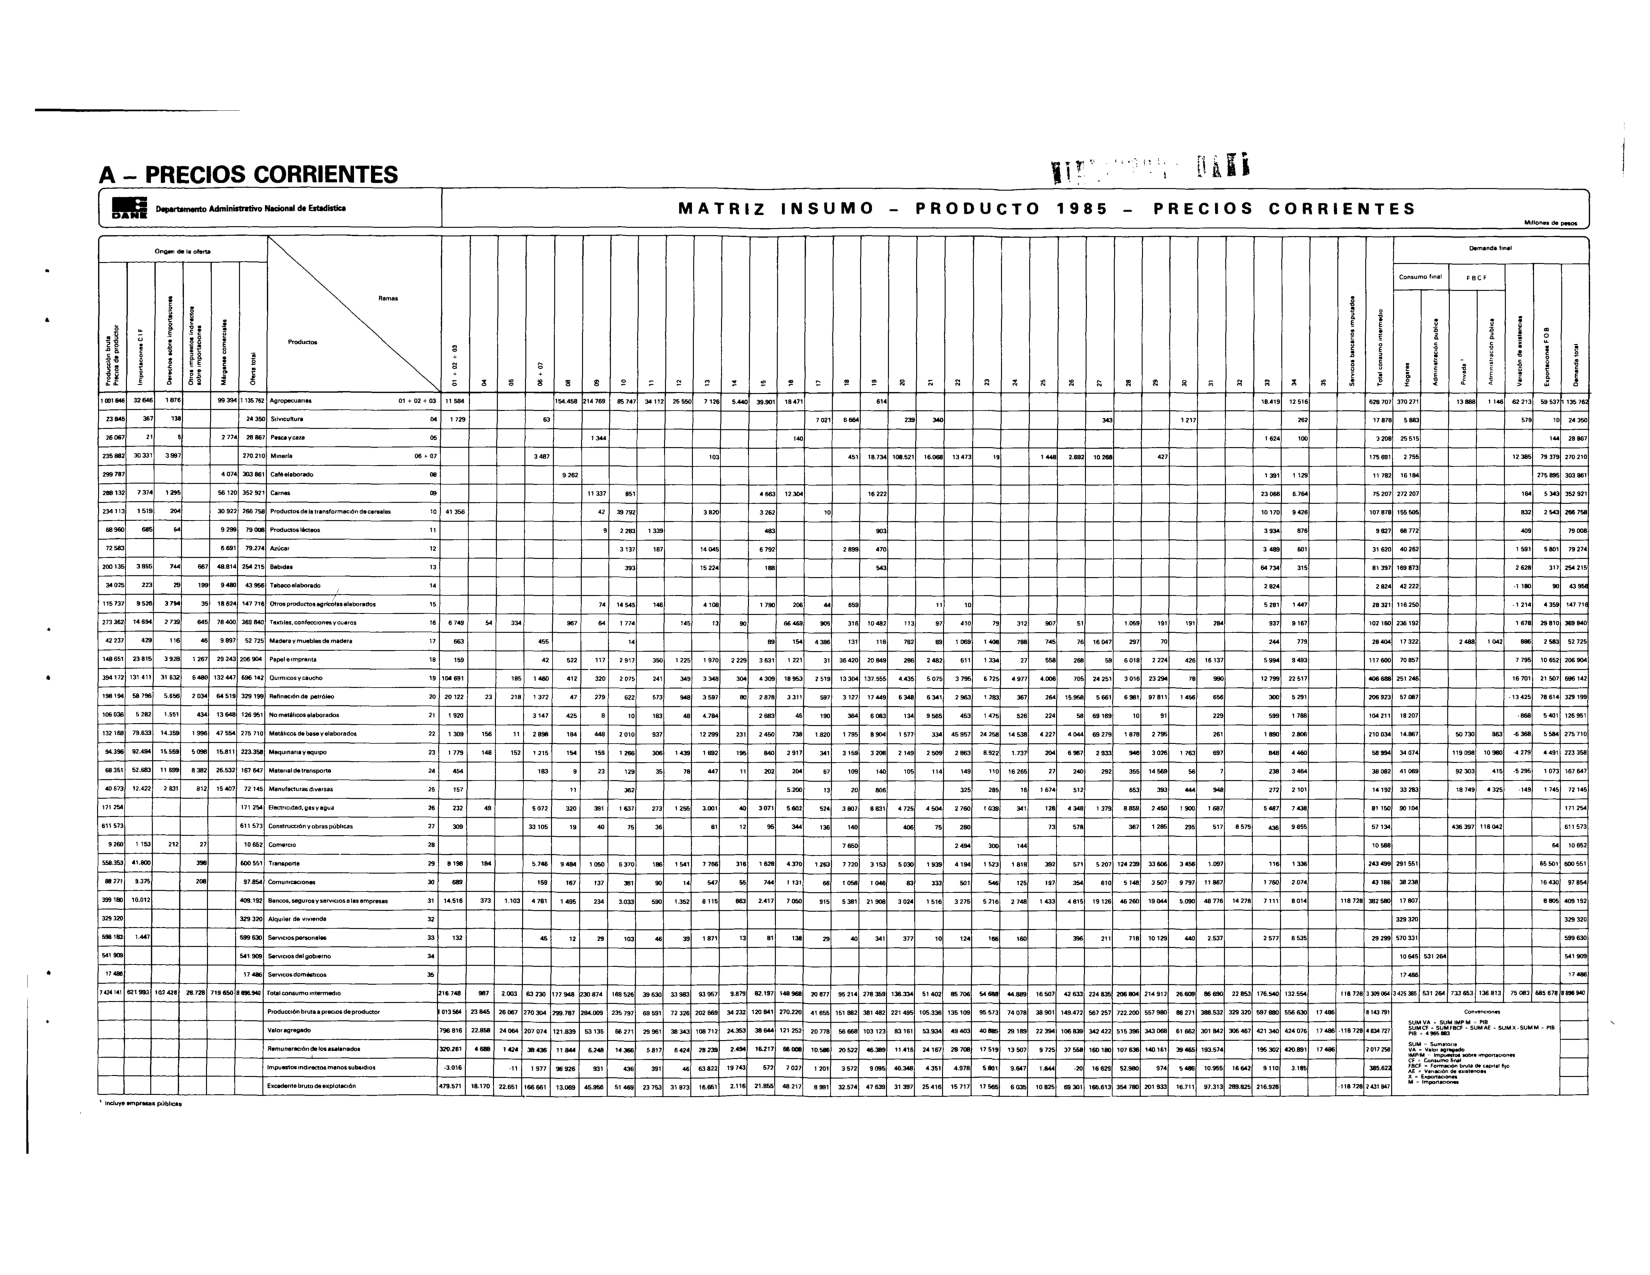
\includegraphics[width=0.9\textwidth,height=\textheight]{images/tables/COL-Mat-InsProd-1985.pdf}

}

\caption{IO-Matrix 1985 Colombia}

\end{figure}%

}

\caption{\label{fig-io-mat-1985}}

\end{figure}%

\begin{table}

\caption{\label{tbl-comp-test}Comparison of different methods to
estimate the bias corrected confidence intervals and the p-values. The
null hypothesis states that firms do not commit tax evasion through
cost-overreporting. The alternative is that they do. The first column is
a difference of the means test (includes error of the estimator, but
assumes independence of the samples). The different methods showon in
the rest of the columns are combinations of two different procedures
when sampling the bootstrap ---sampling from corporations and
non-corporations, or sampling full data--- and two different methods to
estimate the coefficient of the test --- using all the firms or only the
non-incorporated firms. When not fixing the number of corporations,
Bayesian sampling was used to ensure there would be at least one
corporation needed to estimate the first-stage parameter. The numbers in
parenthesis are the standard errors of the mean difference test. The
numbers in brackets represent the bias-corrected bootstrap confidence
intervals at 95\% significance level. *, **, *** denote significance at
the 10\%, 5\%, and 1\% levels (one-sided).}

\centering{

\centering
\begin{tabular}[t]{r|l|l|l|l|l}
\hline
\multicolumn{2}{c|}{ } & \multicolumn{4}{c}{Bootstrap} \\
\cline{3-6}
\multicolumn{2}{c|}{ } & \multicolumn{2}{c|}{Two Group Sampling} & \multicolumn{2}{c}{Bayesian} \\
\cline{3-4} \cline{5-6}
SIC & Mean Diff. & All & Others & All  & Others \\
\hline
 & 0.02** & 0.02* & 0.02* & 0.02 & 0.02\\
\cline{2-6}
\multirow[t]{-2}{*}{\raggedleft\arraybackslash 311} & (0.011) & [-0.01, 0.06] & [-0.01, 0.08] & [-0.03, 0.07] & [-0.04, 0.08]\\
\cline{1-6}
 & -0.01 & -0.01 & -0.01 & -0.01 & -0.01\\
\cline{2-6}
\multirow[t]{-2}{*}{\raggedleft\arraybackslash 312} & (0.034) & [-0.09, 0.11] & [-0.15, 0.14] & [-0.16, 0.12] & [-0.2, 0.15]\\
\cline{1-6}
 & 0.18*** & 0.07*** & 0.18*** & 0.07** & 0.18***\\
\cline{2-6}
\multirow[t]{-2}{*}{\raggedleft\arraybackslash 313} & (0.026) & [0.03, 0.12] & [0.05, 0.32] & [0.01, 0.12] & [0.03, 0.34]\\
\cline{1-6}
 & 0.13*** & 0.11*** & 0.13*** & 0.11*** & 0.13***\\
\cline{2-6}
\multirow[t]{-2}{*}{\raggedleft\arraybackslash 321} & (0.018) & [0.06, 0.19] & [0.09, 0.24] & [0.02, 0.18] & [0.02, 0.25]\\
\cline{1-6}
 & 0.2*** & 0.2*** & 0.2*** & 0.2** & 0.2**\\
\cline{2-6}
\multirow[t]{-2}{*}{\raggedleft\arraybackslash 322} & (0.039) & [0.06, 0.32] & [0.07, 0.32] & [0.03, 0.35] & [-0.03, 0.36]\\
\cline{1-6}
 & -0.19 & -0.15 & -0.19 & -0.15 & -0.19\\
\cline{2-6}
\multirow[t]{-2}{*}{\raggedleft\arraybackslash 323} & (0.026) & [-0.24, -0.07] & [-0.26, -0.08] & [-0.26, -0.05] & [-0.35, -0.08]\\
\cline{1-6}
 & 0.07** & 0.07** & 0.07** & 0.07 & 0.07\\
\cline{2-6}
\multirow[t]{-2}{*}{\raggedleft\arraybackslash 324} & (0.03) & [-0.02, 0.23] & [-0.01, 0.23] & [-0.07, 0.24] & [-0.07, 0.25]\\
\cline{1-6}
 & 0.24*** & 0.22*** & 0.24*** & 0.22** & 0.24**\\
\cline{2-6}
\multirow[t]{-2}{*}{\raggedleft\arraybackslash 331} & (0.044) & [0.05, 0.42] & [0.04, 0.47] & [-0.06, 0.42] & [0, 0.49]\\
\cline{1-6}
 & -0.03 & -0.03 & -0.03 & -0.03 & -0.03\\
\cline{2-6}
\multirow[t]{-2}{*}{\raggedleft\arraybackslash 332} & (0.057) & [-0.24, 0.18] & [-0.27, 0.2] & [-0.28, 0.27] & [-0.42, 0.27]\\
\cline{1-6}
 & -0.05 & -0.03 & -0.05 & -0.03 & -0.05\\
\cline{2-6}
\multirow[t]{-2}{*}{\raggedleft\arraybackslash 341} & (0.024) & [-0.12, 0.05] & [-0.17, 0.06] & [-0.12, 0.06] & [-0.18, 0.09]\\
\cline{1-6}
 & 0.07*** & 0.06* & 0.07** & 0.06 & 0.07\\
\cline{2-6}
\multirow[t]{-2}{*}{\raggedleft\arraybackslash 342} & (0.027) & [-0.01, 0.17] & [-0.02, 0.19] & [-0.08, 0.18] & [-0.09, 0.19]\\
\cline{1-6}
 & 0.09** & 0.03 & 0.09 & 0.03 & 0.09\\
\cline{2-6}
\multirow[t]{-2}{*}{\raggedleft\arraybackslash 351} & (0.046) & [-0.04, 0.11] & [-0.13, 0.33] & [-0.06, 0.12] & [-0.18, 0.39]\\
\cline{1-6}
 & 0.06*** & 0.04** & 0.06** & 0.04 & 0.06\\
\cline{2-6}
\multirow[t]{-2}{*}{\raggedleft\arraybackslash 352} & (0.017) & [0, 0.1] & [-0.01, 0.16] & [-0.03, 0.1] & [-0.05, 0.15]\\
\cline{1-6}
 & -0.1 & -0.08 & -0.1 & -0.08 & -0.1\\
\cline{2-6}
\multirow[t]{-2}{*}{\raggedleft\arraybackslash 356} & (0.018) & [-0.15, -0.04] & [-0.17, -0.05] & [-0.15, -0.01] & [-0.19, 0]\\
\cline{1-6}
 & 0.2*** & 0.14*** & 0.2*** & 0.14** & 0.2**\\
\cline{2-6}
\multirow[t]{-2}{*}{\raggedleft\arraybackslash 369} & (0.036) & [0.05, 0.3] & [0.06, 0.43] & [0, 0.27] & [0, 0.38]\\
\cline{1-6}
 & -0.01 & -0.01 & -0.01 & -0.01 & -0.01\\
\cline{2-6}
\multirow[t]{-2}{*}{\raggedleft\arraybackslash 381} & (0.017) & [-0.06, 0.05] & [-0.09, 0.07] & [-0.08, 0.09] & [-0.11, 0.08]\\
\cline{1-6}
 & -0.02 & -0.02 & -0.02 & -0.02 & -0.02\\
\cline{2-6}
\multirow[t]{-2}{*}{\raggedleft\arraybackslash 382} & (0.026) & [-0.08, 0.09] & [-0.09, 0.08] & [-0.12, 0.06] & [-0.13, 0.07]\\
\cline{1-6}
 & 0.04** & 0.03 & 0.04 & 0.03 & 0.04\\
\cline{2-6}
\multirow[t]{-2}{*}{\raggedleft\arraybackslash 383} & (0.025) & [-0.03, 0.11] & [-0.04, 0.17] & [-0.06, 0.12] & [-0.1, 0.17]\\
\cline{1-6}
 & -0.13 & -0.1 & -0.13 & -0.1 & -0.13\\
\cline{2-6}
\multirow[t]{-2}{*}{\raggedleft\arraybackslash 384} & (0.029) & [-0.19, 0.01] & [-0.24, 0.01] & [-0.21, 0.02] & [-0.3, 0.02]\\
\cline{1-6}
 & 0.04 & 0.04 & 0.04 & 0.04 & 0.04\\
\cline{2-6}
\multirow[t]{-2}{*}{\raggedleft\arraybackslash 390} & (0.046) & [-0.13, 0.25] & [-0.15, 0.24] & [-0.17, 0.27] & [-0.23, 0.31]\\
\hline
\end{tabular}

}

\end{table}%

\begin{table}

\caption{\label{tbl-sec11-inds-char-coprs-vs-others}Comparison of
industry characteristics between corporations and non-corporations.}

\centering{

\centering
\begin{tabular}[t]{r|r|r|r|r|r|r|r|r|r|r|r|r|r|r|r|r|r|r}
\hline
\multicolumn{1}{c|}{ } & \multicolumn{2}{c|}{N} & \multicolumn{2}{c|}{Avg. Age} & \multicolumn{2}{c|}{Sales (Sales Tax Rate)} & \multicolumn{2}{c|}{Purchases (Sales Tax Rate)} & \multicolumn{2}{c|}{Mkt \% (Sales)} & \multicolumn{2}{c|}{Exports (Avg. \%)} & \multicolumn{2}{c|}{Imports (Avg. \%)} & \multicolumn{2}{c|}{Exporters (N \%)} & \multicolumn{2}{c}{Importers (N \%)} \\
\cline{2-3} \cline{4-5} \cline{6-7} \cline{8-9} \cline{10-11} \cline{12-13} \cline{14-15} \cline{16-17} \cline{18-19}
SIC & Corp's & Others & Corp's & Others & Corp's & Others & Corp's & Others & Corp's & Others & Corp's & Others & Corp's & Others & Corp's & Others & Corp's & Others\\
\hline
311 & 147 & 783 & 27 & 20 & 0.5 & 0.1 & 0.9 & 0.4 & 15.2 & 8.4 & 5.4 & 4.3 & 17.5 & 6.1 & 27.0 & 5.7 & 55.4 & 11.2\\
\hline
312 & 41 & 161 & 26 & 21 & 0.2 & 0.2 & 1.2 & 0.7 & 3.9 & 1.4 & 6.4 & 1.3 & 11.9 & 5.1 & 28.4 & 4.5 & 75.7 & 20.4\\
\hline
313 & 74 & 61 & 31 & 31 & 4.5 & 14.8 & 1.6 & 3.5 & 7.7 & 2.0 & 0.1 & 0.3 & 10.6 & 3.1 & 0.4 & 9.8 & 49.6 & 35.6\\
\hline
321 & 71 & 422 & 26 & 17 & 8.2 & 8.0 & 3.8 & 4.8 & 5.1 & 2.4 & 4.3 & 2.0 & 20.3 & 5.4 & 46.6 & 11.5 & 64.5 & 18.8\\
\hline
322 & 22 & 724 & 24 & 14 & 7.9 & 8.1 & 4.1 & 4.6 & 0.5 & 2.0 & 13.6 & 3.2 & 6.2 & 1.6 & 64.6 & 9.8 & 37.2 & 5.5\\
\hline
323 & 13 & 90 & 35 & 17 & 6.5 & 8.5 & 4.8 & 5.0 & 0.7 & 0.5 & 28.0 & 13.4 & 9.4 & 3.9 & 80.2 & 35.1 & 82.1 & 28.7\\
\hline
324 & 9 & 186 & 35 & 14 & 8.1 & 8.0 & 5.5 & 4.8 & 0.6 & 0.4 & 16.4 & 2.9 & 7.7 & 1.0 & 93.2 & 10.7 & 91.5 & 10.6\\
\hline
331 & 13 & 160 & 21 & 18 & 6.6 & 5.5 & 1.9 & 1.8 & 0.4 & 0.2 & 6.0 & 1.6 & 3.8 & 1.4 & 49.0 & 4.4 & 38.5 & 7.6\\
\hline
332 & 12 & 187 & 25 & 15 & 9.5 & 10.6 & 4.3 & 4.0 & 0.1 & 0.2 & 5.0 & 0.5 & 7.7 & 1.2 & 19.3 & 3.3 & 29.8 & 6.7\\
\hline
341 & 41 & 119 & 26 & 20 & 8.7 & 9.1 & 3.8 & 5.0 & 4.5 & 0.6 & 4.9 & 0.2 & 21.1 & 2.6 & 43.3 & 5.2 & 60.1 & 14.6\\
\hline
342 & 40 & 324 & 25 & 22 & 5.1 & 8.0 & 2.9 & 3.8 & 1.3 & 1.6 & 8.4 & 1.3 & 34.7 & 9.3 & 42.6 & 7.7 & 76.2 & 25.1\\
\hline
351 & 68 & 55 & 24 & 17 & 7.3 & 6.4 & 3.0 & 3.6 & 6.5 & 0.9 & 7.0 & 3.2 & 30.3 & 14.3 & 54.2 & 21.7 & 72.1 & 48.7\\
\hline
352 & 100 & 216 & 30 & 24 & 7.1 & 6.7 & 3.8 & 3.8 & 7.3 & 1.2 & 2.0 & 1.1 & 45.5 & 20.0 & 52.6 & 10.4 & 96.2 & 56.4\\
\hline
356 & 53 & 241 & 20 & 15 & 9.6 & 10.2 & 5.7 & 6.1 & 2.1 & 1.3 & 5.6 & 1.8 & 37.7 & 15.7 & 53.4 & 17.3 & 86.1 & 40.5\\
\hline
369 & 58 & 223 & 29 & 19 & 4.9 & 5.7 & 1.7 & 2.0 & 3.0 & 0.4 & 4.2 & 0.4 & 12.9 & 5.9 & 29.4 & 4.1 & 39.7 & 19.2\\
\hline
381 & 85 & 569 & 24 & 17 & 9.0 & 9.4 & 4.8 & 4.9 & 2.6 & 1.4 & 5.3 & 1.2 & 30.3 & 12.8 & 52.8 & 9.8 & 78.0 & 32.2\\
\hline
382 & 46 & 330 & 26 & 20 & 8.1 & 7.8 & 4.2 & 4.0 & 1.0 & 0.9 & 6.4 & 3.7 & 39.1 & 13.9 & 54.7 & 18.3 & 85.7 & 43.5\\
\hline
383 & 57 & 168 & 23 & 18 & 9.3 & 8.8 & 4.5 & 4.6 & 3.1 & 0.8 & 3.5 & 2.0 & 52.1 & 23.8 & 49.2 & 13.5 & 95.3 & 57.3\\
\hline
384 & 42 & 209 & 26 & 17 & 8.7 & 7.4 & 5.0 & 5.0 & 5.9 & 0.9 & 5.2 & 2.0 & 48.4 & 14.5 & 39.8 & 8.8 & 80.3 & 38.7\\
\hline
390 & 18 & 163 & 24 & 21 & 9.6 & 11.4 & 4.1 & 4.1 & 0.4 & 0.5 & 15.1 & 3.1 & 43.6 & 13.6 & 82.3 & 19.6 & 90.3 & 40.7\\
\hline
\end{tabular}

}

\end{table}%

\begin{table}

\caption{\label{tbl-tims-test}Rejection frequencies of the
\(\mathcal{V}_{it}\) for Corporations and Non-Corporations. The
rejection frequencies of the one tail test are the average number of
observations that fell above the 95\% region of the
\(f_{\varepsilon}(\varepsilon)\) distribution recovered in the first
stage. The rejection frequencies of the two tail test are the average
number of observations that fell above the 97.5\% or below the 2.5\%
region.}

\centering{

\centering
\begin{tabular}[t]{l|r|r|r|r}
\hline
\multicolumn{1}{c|}{ } & \multicolumn{2}{c|}{One Tail} & \multicolumn{2}{c}{Two Tail} \\
\cline{2-3} \cline{4-5}
SIC & Corp & Non-Corp & Corp  & Non-Corp \\
\hline
311 & 5.1 & 9.3 & 5.1 & 8.7\\
\cline{1-5}
312 & 5.1 & 3.2 & 5.1 & 6.8\\
\cline{1-5}
322 & 4.4 & 26.3 & 3.5 & 8.9\\
\cline{1-5}
381 & 4.9 & 4.6 & 4.9 & 6.3\\
\cline{1-5}
321 & 4.9 & 21.4 & 5.1 & 12.7\\
\cline{1-5}
382 & 5.0 & 5.2 & 5.0 & 5.4\\
\cline{1-5}
384 & 5.0 & 0.6 & 4.7 & 4.3\\
\cline{1-5}
383 & 4.9 & 2.6 & 5.1 & 2.9\\
\cline{1-5}
313 & 5.0 & 17.9 & 5.0 & 12.9\\
\cline{1-5}
341 & 5.0 & 4.4 & 5.0 & 8.1\\
\cline{1-5}
324 & 5.1 & 10.4 & 5.1 & 11.2\\
\cline{1-5}
342 & 5.1 & 6.3 & 5.1 & 5.9\\
\cline{1-5}
369 & 5.1 & 12.5 & 4.8 & 12.8\\
\cline{1-5}
332 & 5.3 & 4.3 & 5.3 & 8.5\\
\cline{1-5}
390 & 4.4 & 1.1 & 4.4 & 1.0\\
\cline{1-5}
351 & 4.8 & 11.2 & 4.8 & 10.5\\
\cline{1-5}
352 & 4.9 & 12.1 & 5.0 & 9.9\\
\cline{1-5}
356 & 5.2 & 3.9 & 5.2 & 8.6\\
\cline{1-5}
331 & 5.8 & 26.1 & 4.8 & 22.7\\
\cline{1-5}
323 & 4.7 & 1.5 & 3.8 & 12.6\\
\hline
\end{tabular}

}

\end{table}%

\subsection{Production Function}\label{production-function}

Table~\ref{tbl-CD-ar1-comparision} displays the results of estimating
the production function parameters following the identification strategy
described above. I use an AR(1) model for the Markov process of
productivity. I employed \(Z=\{k_{it},l_{it}\}\) as instruments for
themselves. One additional instrument to control for the endogeneity
between \(\varepsilon_{it-1}\) and \(\mathcal{W}_{it-1}\) is needed in
the first stage of `TE+GNR'. The instrument used is specified in the
table Table~\ref{tbl-CD-ar1-comparision}.

To compare, I also include the uncorrected estimates using GNR and a
simple OLS. In the case of GNR estimation method, the Markov process of
productivity is a third degree polynomial, and capital and labor, the
instruments.

I focus on the top 5 industries in terms of revenue: 1) 311 - Food
Products, 2) 313 Beverages, 3) 352 Other Chemical Products. 4) 351
Industrial Chemicals, and 5) 321 Textiles.

\begin{table}

\caption{\label{tbl-CD-ar1-comparision}Cobb-Douglas production function
parameters estimates, correcting intermediates ---raw materials--- for
tax evasion vs.~naive estimation and OLS. \(h\) is an AR(1) process for
`Tax Evasion + GNR' but a third degree polynomial for `GNR'.
\(Z=\{k_{it},l_{it}\}\) for GNR. One additional instrument to GNR's
\(Z\) control for the endogeneity between \(\varepsilon_{it-1}\) and
\(\mathcal{W}_{it-1}\) in the first stage of `TE+GNR'. The instrument
used is specified in the table.}

\centering{

\centering
\begin{tabular}[t]{l|l|r|r|r|r|r|r}
\hline
\multicolumn{2}{c|}{ } & \multicolumn{4}{c|}{Tax Evasion + GNR} & \multicolumn{2}{c}{ } \\
\cline{3-6}
Inds. & Input & \$k\_\{it-1\}\$ & \$l\_\{it-1\}\$ & \$m\textasciicircum{}*\_\{it-1\}\$ & \$\textbackslash{}mathcal\{W\}\_\{it-2\}\$ & GNR &  OLS\\
\hline
 & m & 0.2937 & 0.2937 & 0.2937 & 0.2937 & 0.3485 & 0.5593\\
\cline{2-8}
 & k & 0.0388 & 0.0000 & 0.1156 & 0.0721 & 0.1043 & 0.0636\\
\cline{2-8}
\multirow[t]{-3}{*}{\raggedright\arraybackslash 331} & l & 0.5819 & 0.3383 & 0.6179 & 0.5809 & 0.5063 & 0.4311\\
\cline{1-8}
 & m & 0.3123 & 0.3123 & 0.3123 & 0.3123 & 0.3683 & 0.5669\\
\cline{2-8}
 & k & 0.0911 & 0.0540 & 0.1698 & 0.1875 & 0.1921 & 0.0477\\
\cline{2-8}
\multirow[t]{-3}{*}{\raggedright\arraybackslash 322} & l & 0.3125 & 0.2986 & 0.4076 & 0.4106 & 0.3608 & 0.4119\\
\cline{1-8}
 & m & 0.1999 & 0.1999 & 0.1999 & 0.1999 & 0.2252 & 0.4974\\
\cline{2-8}
 & k & 0.0526 & 0.3351 & 1.0000 & 0.3492 & 0.2652 & 0.1253\\
\cline{2-8}
\multirow[t]{-3}{*}{\raggedright\arraybackslash 369} & l & 0.5524 & 0.3619 & 0.8056 & 0.5831 & 0.6055 & 0.5206\\
\cline{1-8}
 & m & 0.2701 & 0.2701 & 0.2701 & 0.2701 & 0.2826 & 0.7497\\
\cline{2-8}
 & k & 0.0160 & 1.0000 & 0.4610 & 0.0000 & 0.3395 & 0.1171\\
\cline{2-8}
\multirow[t]{-3}{*}{\raggedright\arraybackslash 313} & l & 0.0283 & 0.1592 & 0.1229 & 0.2157 & 0.2943 & 0.2702\\
\cline{1-8}
 & m & 0.3544 & 0.3544 & 0.3544 & 0.3544 & 0.3869 & 0.6616\\
\cline{2-8}
 & k & 0.0697 & 0.0000 & 0.3389 & 0.3214 & 0.2604 & 0.0966\\
\cline{2-8}
\multirow[t]{-3}{*}{\raggedright\arraybackslash 321} & l & 0.1324 & 0.2780 & 0.2987 & 0.3383 & 0.3412 & 0.2796\\
\hline
\end{tabular}

}

\end{table}%

\begin{table}

\caption{\label{tbl-CD-ar1-comparision-me}Cobb-Douglas production
function parameters estimates, correcting intermediates ---raw
materials--- for tax evasion vs.~naive estimation and OLS. \(h\) is an
AR(1) process for `Tax Evasion + GNR' but a third degree polynomial for
`GNR'. \(Z=\{k_{it},l_{it}\}\) for GNR. One additional instrument to
GNR's \(Z\) control for the endogeneity between \(\varepsilon_{it-1}\)
and \(\mathcal{W}_{it-1}\) in the first stage of `TE+GNR'. The
instrument used is specified in the table. \(\varepsilon_{it-1}\) is
defined as measurement error.}

\centering{

\centering
\begin{tabular}[t]{l|l|r|r|r|r|r|r}
\hline
\multicolumn{2}{c|}{ } & \multicolumn{4}{c|}{Tax Evasion + GNR} & \multicolumn{2}{c}{ } \\
\cline{3-6}
Inds. & Input & \$k\_\{it-1\}\$ & \$l\_\{it-1\}\$ & \$m\textasciicircum{}*\_\{it-1\}\$ & \$\textbackslash{}mathcal\{W\}\_\{it-2\}\$ & GNR &  OLS\\
\hline
 & m & 0.3209 & 0.3209 & 0.3209 & 0.3209 & 0.3989 & 0.5593\\
\cline{2-8}
 & k & 0.0373 & 0.0000 & 0.1112 & 0.0693 & 0.0962 & 0.0636\\
\cline{2-8}
\multirow[t]{-3}{*}{\raggedright\arraybackslash 331} & l & 0.5596 & 0.3253 & 0.5941 & 0.5587 & 0.4671 & 0.4311\\
\cline{1-8}
 & m & 0.3469 & 0.3469 & 0.3469 & 0.3469 & 0.4218 & 0.5669\\
\cline{2-8}
 & k & 0.0865 & 0.0520 & 0.1612 & 0.1781 & 0.1759 & 0.0477\\
\cline{2-8}
\multirow[t]{-3}{*}{\raggedright\arraybackslash 322} & l & 0.2968 & 0.2837 & 0.3871 & 0.3900 & 0.3302 & 0.4119\\
\cline{1-8}
 & m & 0.2441 & 0.2441 & 0.2441 & 0.2441 & 0.2821 & 0.4974\\
\cline{2-8}
 & k & 0.0497 & 0.3166 & 1.0000 & 0.3290 & 0.2457 & 0.1253\\
\cline{2-8}
\multirow[t]{-3}{*}{\raggedright\arraybackslash 369} & l & 0.5218 & 0.3419 & 0.7503 & 0.5528 & 0.5611 & 0.5206\\
\cline{1-8}
 & m & 0.2894 & 0.2894 & 0.2894 & 0.2894 & 0.3091 & 0.7497\\
\cline{2-8}
 & k & 0.0155 & 1.0000 & 0.4489 & 0.0000 & 0.3270 & 0.1171\\
\cline{2-8}
\multirow[t]{-3}{*}{\raggedright\arraybackslash 313} & l & 0.0276 & 0.1531 & 0.1197 & 0.2100 & 0.2834 & 0.2702\\
\cline{1-8}
 & m & 0.3869 & 0.3869 & 0.3869 & 0.3869 & 0.4316 & 0.6616\\
\cline{2-8}
 & k & 0.0662 & 0.0000 & 0.3218 & 0.3052 & 0.2414 & 0.0966\\
\cline{2-8}
\multirow[t]{-3}{*}{\raggedright\arraybackslash 321} & l & 0.1257 & 0.2640 & 0.2838 & 0.3213 & 0.3163 & 0.2796\\
\hline
\end{tabular}

}

\end{table}%

\begin{table}

\caption{\label{tbl-1s-diagnostics}First stage `Weak Instruments' F-test
of the 2SLS-IV estimation. The null hypothesis is that the coefficients
are equal to zero, in other words, uncorrelated with the endogenous
variable \(\mathcal{W}_{it-1}\).}

\centering{

\centering
\begin{tabular}[t]{l|l|l|l|r|r|l}
\hline
Ins. & Inds. & df1 & df2 & statistic & p-value & stars\\
\hline
 & 331 & 1 & 785 & 121.4029 & 0 & ***\\
\cline{2-7}
 & 322 & 1 & 3581 & 1419.5262 & 0 & ***\\
\cline{2-7}
 & 369 & 1 & 1235 & 1764.8363 & 0 & ***\\
\cline{2-7}
 & 313 & 1 & 985 & 2758.2637 & 0 & ***\\
\cline{2-7}
\multirow[t]{-5}{*}{\raggedright\arraybackslash \$k\_\{t-1\}\$} & 321 & 1 & 2339 & 3714.9184 & 0 & ***\\
\cline{1-7}
 & 331 & 1 & 785 & 778.9743 & 0 & ***\\
\cline{2-7}
 & 322 & 1 & 3581 & 3840.2193 & 0 & ***\\
\cline{2-7}
 & 369 & 1 & 1235 & 308.5926 & 0 & ***\\
\cline{2-7}
 & 313 & 1 & 985 & 435.1505 & 0 & ***\\
\cline{2-7}
\multirow[t]{-5}{*}{\raggedright\arraybackslash \$l\_\{t-1\}\$} & 321 & 1 & 2339 & 4176.4138 & 0 & ***\\
\cline{1-7}
 & 331 & 1 & 785 & 416.9415 & 0 & ***\\
\cline{2-7}
 & 322 & 1 & 3581 & 4963.1390 & 0 & ***\\
\cline{2-7}
 & 369 & 1 & 1235 & 1048.3330 & 0 & ***\\
\cline{2-7}
 & 313 & 1 & 985 & 458.2628 & 0 & ***\\
\cline{2-7}
\multirow[t]{-5}{*}{\raggedright\arraybackslash \$m\textasciicircum{}*\_\{t-1\}\$} & 321 & 1 & 2339 & 420.5456 & 0 & ***\\
\cline{1-7}
 & 331 & 1 & 636 & 1961.0846 & 0 & ***\\
\cline{2-7}
 & 322 & 1 & 2949 & 8673.2398 & 0 & ***\\
\cline{2-7}
 & 369 & 1 & 1004 & 3778.8152 & 0 & ***\\
\cline{2-7}
 & 313 & 1 & 865 & 24073.3213 & 0 & ***\\
\cline{2-7}
\multirow[t]{-5}{*}{\raggedright\arraybackslash \$\textbackslash{}mathcal\{W\}\_\{t-2\}\$} & 321 & 1 & 1959 & 7279.2133 & 0 & ***\\
\hline
\end{tabular}

}

\end{table}%

From Table~\ref{tbl-1s-diagnostics}, we can conclude that \(m^*_{t-1}\)
is a better than \(\mathcal{W}_{t-2}\), \(k_{t-1}\) and \(l_{t-1}\). The
following discussion will be focusing on the results relating using
\(m^*_{t-1}\) as the instrument.

First, because tax evasion artificially inflates the intermediates's
cost share of revenues, lower output elasticities of intermediates than
traditional methods are expected. In table
Table~\ref{tbl-CD-ar1-comparision} shows that correcting for tax evasion
results in smaller intermediates' output elasticity with respect with
OLS. With respect to GNR, all estimates are statistically lower except
one. The output elasticity of intermediates of the Textile industry
(321) is significantly greater than the GNR result.

Three of the five intermediate elasticities resulted as not
statistically different from zero. These zeros are not exclusive to the
method correcting by tax evasion, as we can see that GNR for
Cobb-Douglas approach zero for some industries. These zeros could be the
result of the functional form. A Cobb-Douglas specification leaves out
the cross-elasticities which could lead to omitted variables bias. In
other words, we effectively ignore complementarity or substitutability
between the inputs. This CD omitted variable bias could be accentutated
because we defined raw materials as intermediates leaving out others,
such as energy, fuels, and services.

The elasticities of capital and labor vary across industries, with some
being lower, some higher, and others quite similar. This is expected.
The direction of the bias in the elasticities of capital and labor
depends on whether thse inputs are complements or subsitutes of
intermediate inputs. This relatioship will vary by industry. Put
differently, for different industries, the cross-elasticity between
intermediates and capital, and intermediates and labor will be different
in direction and magnitude. Since these cross-elasticities are not
included in the CD production function, the elasticities of capital and
labor should reflect different degrees of these variations once
intermediates are corrected for overreporting.

\subsection{Productivity}\label{productivity}

Once, the production function parameters are known, we can recover
\(\omega\) by deconvolution using Equation~\ref{eq-w-squiggle}. Here I
assume \(\omega\) follows a normal distribution.

\textbf{?@tbl-boot-omega} displays the estimates of the distribution
parameters of \(\omega\) corresponding to the instrument used in the
previous section and the parametric specification of an AR(1).

\begin{table}

\caption{\label{tbl-omega}Estimates Omega Distribution by Industry after
Deconvoluting from the Output Shock.}

\centering{

\centering
\begin{tabular}[t]{r|r|r}
\hline
  & \$\textbackslash{}mu\$ & \$\textbackslash{}sigma\$\\
\hline
322 & 5.43 & 0.58\\
\hline
342 & 4.25 & 0.47\\
\hline
313 & 3.29 & 0.45\\
\hline
351 & 3.47 & 0.65\\
\hline
331 & 4.04 & 0.38\\
\hline
\end{tabular}

}

\end{table}%

To compare these productivity estimates to uncorrected ones, I simulate
productivity using the parameters estimated in
\textbf{?@tbl-boot-omega}. I use 1000 independent draws from \(\omega\)
and \(\varepsilon\). Then, I computed productivity,
\(\varphi_{it}^S=\exp\{\omega_{it}^S+\varepsilon_{it}^S\}\).

Table~\ref{tbl-prod-comparison} compares summary statistics the
simulated productivity using the estimated parameters after correcting
for tax evasion with the summary statistics of the productivity
estimates of GNR.

\begin{table}

\caption{\label{tbl-prod-comparison}Summary statistics of the
productivity estimates using GNR correcting and not correcting for tax
evasion. Tax-evasion corrected estimates were simulated using the
parameters of \textbf{?@tbl-boot-omega}, with 1000 draws.}

\centering{

\centering
\begin{tabular}[t]{r|l|r|r|r|r|r}
\hline
inds & Method & Mean & SD & Q1 & Median & Q3\\
\hline
 & GNR & 70.6 & 44.7 & 45.1 & 59.0 & 82.7\\
\cline{2-7}
\multirow[t]{-2}{*}{\raggedleft\arraybackslash 313} & TE: \$m\textasciicircum{}*\_\{t-1\}\$ & 55.8 & 39.9 & 29.3 & 47.0 & 70.2\\
\cline{1-7}
 & GNR & 23.6 & 11.0 & 17.4 & 21.5 & 27.3\\
\cline{2-7}
\multirow[t]{-2}{*}{\raggedleft\arraybackslash 321} & TE: \$m\textasciicircum{}*\_\{t-1\}\$ & 21.6 & 13.1 & 12.6 & 18.2 & 26.7\\
\cline{1-7}
 & GNR & 41.6 & 14.3 & 32.2 & 39.1 & 48.6\\
\cline{2-7}
\multirow[t]{-2}{*}{\raggedleft\arraybackslash 322} & TE: \$m\textasciicircum{}*\_\{t-1\}\$ & 83.1 & 54.5 & 47.2 & 68.1 & 106.0\\
\cline{1-7}
 & GNR & 61.1 & 23.5 & 46.3 & 56.5 & 70.3\\
\cline{2-7}
\multirow[t]{-2}{*}{\raggedleft\arraybackslash 331} & TE: \$m\textasciicircum{}*\_\{t-1\}\$ & 73.8 & 44.5 & 42.9 & 63.7 & 93.0\\
\cline{1-7}
 & GNR & 23.1 & 8.3 & 18.1 & 21.7 & 26.3\\
\cline{2-7}
\multirow[t]{-2}{*}{\raggedleft\arraybackslash 342} & TE: \$m\textasciicircum{}*\_\{t-1\}\$ & 32.1 & 18.4 & 18.5 & 27.7 & 40.7\\
\hline
\end{tabular}

}

\end{table}%

Industries 321 Textiles, and 351 Industrial Chemicals, and 313 Beverages
have means lower or equal to the uncorrected ones for both instruments
considered. Industry 311 Food Products display a higher mean for both
estimates, while industry 352 Other Chemicals displays a higher or lower
mean depending on the instrument.

With respect to standard deviations, industries 321 Textiles, 351
Industrial Chemicals, and 352 Other Chemicals display lower magnitudes,
while industries 311 Food Products display significantly higher
magnitudes. Lastly, industry 313 Beverages standard deviation is lower
or higher depending on the instrument.

\subsubsection{Non-Parametric Productivity
Density}\label{non-parametric-productivity-density}

Nothing impedes us from estimating a non-parametric distribution of
\(\omega\). I deconvolute \(\omega\) using penalized B-Splines from
Equation~\ref{eq-w-squiggle}. First, I estimate the density of
\(\varepsilon\) using a kernel density estimator.

\begin{table}

\caption{\label{tbl-np-prod}Non-Parametric Deconvolution of \(\omega\)
using Penalized B-Splines. The error density function is estimated using
a kernel density estimator fitted on the residuals of the first stage
conditional on firms being Non-Evaders.}

\centering{

\centering
\begin{tabular}[t]{l|l|r|r|r}
\hline
sic\_3 & instrument & mean & sd & skewness\\
\hline
331 & \$m\_\{t-1\}\$ & 4.140 & 0.256 & -0.724\\
\hline
322 & \$m\_\{t-1\}\$ & 4.253 & 0.303 & -0.455\\
\hline
369 & \$m\_\{t-1\}\$ & -3.984 & 1.929 & 0.542\\
\hline
313 & \$m\_\{t-1\}\$ & 3.799 & 0.454 & -0.088\\
\hline
321 & \$m\_\{t-1\}\$ & 2.885 & 0.391 & -0.127\\
\hline
331 & \$\textbackslash{}mathcal\{W\}\_\{t-2\}\$ & 4.616 & 0.269 & -0.179\\
\hline
322 & \$\textbackslash{}mathcal\{W\}\_\{t-2\}\$ & 4.102 & 0.297 & -0.481\\
\hline
369 & \$\textbackslash{}mathcal\{W\}\_\{t-2\}\$ & 3.017 & 0.305 & -0.489\\
\hline
313 & \$\textbackslash{}mathcal\{W\}\_\{t-2\}\$ & 8.410 & 0.926 & -0.496\\
\hline
321 & \$\textbackslash{}mathcal\{W\}\_\{t-2\}\$ & 2.885 & 0.378 & -0.069\\
\hline
\end{tabular}

}

\end{table}%

\begin{table}

\caption{\label{tbl-np-sim-prod}Summary statistics of the simulated
productivity using the non-parametric estimates of \(\omega\) and
\(\varepsilon\). Both functions were numerically inverted to obtain
simulated draws of \(\omega\) and \(\varepsilon\). 1000 draws were used.
Productivity is computed as
\(\varphi_{it}^S=\exp{\omega_{it}^S+\varepsilon_{it}^S}\).}

\centering{

\centering
\begin{tabular}[t]{r|l|r|r|r|r|r}
\hline
sic\_3 & Method & Mean & SD & Q1 & Median & Q3\\
\hline
313 & TE: \$\textbackslash{}mathcal\{W\}\_\{t-2\}\$ & 6841.3 & 7504.3 & 2457.8 & 4928.0 & 8309.3\\
\hline
313 & TE: \$m\textasciicircum{}*\_\{t-1\}\$ & 52.5 & 37.7 & 30.5 & 44.3 & 63.2\\
\hline
321 & TE: \$\textbackslash{}mathcal\{W\}\_\{t-2\}\$ & 20.8 & 17.1 & 12.7 & 16.8 & 23.1\\
\hline
321 & TE: \$m\textasciicircum{}*\_\{t-1\}\$ & 20.9 & 16.8 & 12.6 & 16.9 & 23.3\\
\hline
322 & TE: \$\textbackslash{}mathcal\{W\}\_\{t-2\}\$ & 68.9 & 50.2 & 42.5 & 56.8 & 78.5\\
\hline
322 & TE: \$m\textasciicircum{}*\_\{t-1\}\$ & 80.4 & 59.1 & 49.3 & 66.3 & 91.7\\
\hline
331 & TE: \$\textbackslash{}mathcal\{W\}\_\{t-2\}\$ & 115.6 & 67.6 & 67.7 & 97.7 & 145.0\\
\hline
331 & TE: \$m\textasciicircum{}*\_\{t-1\}\$ & 71.6 & 40.6 & 42.8 & 60.6 & 89.6\\
\hline
369 & TE: \$\textbackslash{}mathcal\{W\}\_\{t-2\}\$ & 25.4 & 19.3 & 12.1 & 18.0 & 34.4\\
\hline
369 & TE: \$m\textasciicircum{}*\_\{t-1\}\$ & 0.3 & 1.8 & 0.0 & 0.0 & 0.1\\
\hline
\end{tabular}

}

\end{table}%

\section{References}\label{references}

\renewcommand{\bibsection}{}
\bibliography{biblio/export.bib,biblio/export2.bib,biblio/export3.bib,biblio/export31072022.bib,biblio/b100422.bib,biblio/b270123.bib,biblio/b100424.bib}

\section{Tax Evasion and Resource
Missallocation}\label{tax-evasion-and-resource-missallocation}

A popular way to decompose total productivity introduced by
\citet{Olley1996} is the following :

\[
\varphi_t = \bar\varphi_t + \sum_{i=1}^I \left(s_{it}-\bar s_{t}\right)\left(\varphi_{it}-\bar\varphi_t\right)
\]

where \(\varphi_{it}=\exp\{\omega_{it}+\varepsilon_{it}\}\) is the
firm-level productivity, \(s_{it}\) is firm' \(i\) share of output at
time \(t\). \(\bar\varphi_t\) and \(\bar s_t\) represent the unweighted
mean productivity and unweighted mean share.

Intuitively, the more output is allocated to high productivity firms the
higher the total productivity will be. Alternatively, the smaller the
shares allocated to low productivity firms the greater the total
productivity.

Ideally, we would like resources to be allocated to high productivity
firms. Hence, the link between the decomposition of total aggregate
productivity and missallocation.

In the tax evasion context, the productivity of misreporting firms would
look lower than it really is. How would this affect our measures of
total productivity? If misreporting firms have small shares, their
corrected productivity measure might be closer to the mean reducing
their contribution to total productivity, leading to lower measured
levels of total productivity.

In other words, tax evasion through cost overreporting might lead to
biased measures of total aggregate productivity.

However, if we think about the marginal firm that is struggling to stay
in the market, the additional income gained through misreporting might
help her survive longer. Therefore, tax evasion increases missallocation
in the sense that a share of the output is allocated to firms that
otherwise would not be in the market.

There are alternative ways to decompose total productivity that account
for the entry and exit of firms (Foster et al.~2008). In addition,
alternative measures to aggregate productivity have been used elsewhere
(e.g.~aggregate demand shocks in \citet{Eslava2004}).

For example, we can decompose aggregate productivity like this

\[
\Delta\varphi_t = \sum_{i \in C}\bar s_i \Delta\varphi_{it} + \sum_{i\in C}(\bar\varphi_i-\bar\varphi)\Delta s_{it}+\sum_{i\in N} s_{it}\left(\varphi_{it}-\bar\varphi\right)-\sum_{i\in X}s_{it-1}\left(\varphi_{it-1}-\bar \varphi\right)
\]

where \(\Delta\) is the change from \(t-1\) to \(t\), and the sets
\(C\),\(N\), and \(X\) represent the continuing, entering, and exiting
firms.

In the case of corporate tax evasion a relevant measure could be
aggregate profitability. Low productivity firms are surviving not
because they are technologically efficient but because their
profitability is marginally higher when they evade taxes. Decomposing an
aggregate profitability measure by market shares and firm dynamics would
indicate how exiting firms are contributing to the aggregate measure.
Intuitively, again higher levels of aggregate profitability correspond
to larger shares of the market being allocated to high profitability
firms.

In the absence of tax evasion, firms overreporting costs would have
lower after-tax profits. The aggregate profitability level would be
higher if these firms have small market shares and remain in the sample.
On the other hand, the aggregate profitability level would decrease if
the small-share and low-profitability firms were to exit the market.

Therefore, in the case of tax evasion, the key aspect of aggregate
profitability is the counterfactual decision of low-profitability firms
to exit the market in addition to the corrected profits if firms were
not to overreport their costs.

Consequently, the economic model should account for firm entry and exit
along with tax evasion.

\subsection{Implementation}\label{implementation-1}

Given I can only obtain the distribution of productivity
non-parametrically, one way to recover the covariance term between
productivity and size is the following:

\[
Cov(\varphi_{it}, s_{it}) = E[\varphi_{it} s_{it}] - E[\varphi_{it}]E[s_{it}]
\]

Clearly, I can estimate the expectation of \(\varphi_{it}\) and
\(s_{it}\) using the estimated non-parametric distribution. While, I can
directly compute the expectation of size from data.

For the joint expectation, All I need is the conditional distribution of
\(\varphi_{it}\) given \(s_{it}\). This can be estimated
non-parametrically dividing size in different groups, and then
estimating the productivity within each group.

To see this, note that \[
\begin{aligned}
    E[\varphi_{it} s_{it}] &= \int \int \varphi_{it} s_{it} f(\varphi_{it}, s_{it}) d\varphi_{it} ds_{it} \\
    &= \int \left(\int \varphi_{it} s_{it}  f(\varphi_{it}|s_{it}) d\varphi_{it}\right) f(s_{it}) ds_{it}\\
    &= E_{s_{it}}\left[ \left(\int \varphi_{it} s_{it}  f(\varphi_{it}|s_{it}) d\varphi_{it}\right) \right]
\end{aligned}
\]

\section{Lit Review Notes}\label{lit-review-notes}

For personal reference, to be removed from the final version.

\subsection{\texorpdfstring{\citet{Dabla2019}}{@Dabla2019}}\label{dabla2019}

Productivity improvements by firms can causally lead to lower tax
evasion, i.e., underreporting sales for tax purposes. In other words, an
increase in firm productivity leads to a higher share of sales reported
for tax purposes. The authors use the self-reported share of declared
income as a proxy for tax evasion.

Limitations: Using the World Bank Enterprise (47 emerging and developing
countries) survey question to get the percentage of sales that are
reported for tax purposes, which is used to measure tax evasion. In
addition, productivity is measured as the log of sales per worker. No
access to quantities data, they use LP but with sales and workers.

Undisputed (?) facts: 1) Tax evasion is higher in poor countries; 2) Tax
evading firms tend to be less productive (?).

Productivity gaps between firms that comply with taxes and regulations
and those which do not are significant, (between 25 and 50 \%) (Amin et
al.~2019; Fajnzylber, 2011; Busso et al., 2012). These large
productivity gaps can translate into low-economy wide productivity and
growth: 1) if, by not complying with existing taxes and regulations,
firms enjoy a potentially large implicit subsidy that allows them to
stay in business despite low productivity, or 2) to expand their market
share at the expense of more productive firms (Farrell, 2004; Bobbio,
2016).

Almeida and Carneiro (2009): Tax evasion may also increase firms'
efficiency (productivity?). Avoiding onerous taxes might confer firms
more flexibility in their employment and production decisions.

Kleven et. al (2016): Larger firms are less likely to avoid taxes. The
firm's use of business records increases as it hires more employees.
They show that the government may be able to enforce higher tax
compliance even in the presence of a low threat of audit due to the
increased ease of whistleblowing as the firm grows.

Tax evasion is hidden: it is difficult to obtain precise measures (Kundt
et al., 2017; Slemrod and Weber, 2012).

Loayza and Rigolini (2006) and La Porta and Shleifer (2014): informality
is larger in lower GDPpC countries

Tax evasion and informality are associated with lower income levels and
productivity (Dabla-Norris and Feltenstein, 2003; Loayza, 1996; Sarte,
2000)

\subsection{\texorpdfstring{\citet{Paulus2015}}{@Paulus2015}}\label{paulus2015}

The author models discrepancies between tax records and income survey
data as individual tax evasion and measurement error jointly. Using data
for Estonia, the author finds that people in the bottom and the top part
of earnings distribution evade much more and about 12\% of wages and
salaries in total are underreported. The identifying assumption, i.e.,
location condition, is that people working in the public sector cannot
evade taxes. In other words, measurement error is unrelated to the
sector where the individual works while the same does not hold for tax
compliance.

The main constraint for empirical research on tax evasion is the lack of
suitable data. This is worse for developing countries. A measure of
undeclared income for individuals is needed. This kind of data is
usually unreliable and very difficult/or expensive to obtain.

Baldini et al.~(2009) use linked income data with tax records at the
individual level to estimate tax evasion. However, the author assumes
people report their true income in the survey to obtain a measure of
non-reporting. Furthermore, in the measurement error literature, several
studies assume the opposite, e.g.~Krueger (1991) and Bollinger(1998);
survey of lit Chen et al.~(2011) and Bound et al.~(2001). Linked data is
referred to as Validation data in the measurement error literature.
Later studies have started to consider matching errors (Kapteyn and
Ypma, 2007; Meijer et al., 2012) and errors in register data (Abowd and
Stinson, 2013).

Pissarides and Weber (1989) pioneered a methodology to study
underreported income. They assume that the underreported income for one
population group is inferred from a comparison with a reference group
assumed to have negligible non-compliance but to be similar in other
respects. These types of studies assume implicitly that the
underreporting of income in a survey corresponds to the underreporting
of income to the tax authority.

\subsection{\texorpdfstring{\citet{Slemrod2019}}{@Slemrod2019}}\label{slemrod2019}

Tax evasion policies have been a greater priority in developed countries
since the 2008 Great Recession (IMF, 2015). For example, the UK
announced efforts to combat tax avoidance, tax evasion, and `imbalances'
in the tax system that would bring in \pounds 5 billion in additional
revenue each year.

Tax evasion matters because it affects both the resource cost of raising
taxes and the distribution of the tax burden, i.e.~core interests of
public economics. Policy question? Does curbing evasion improve the
equity and efficiency of the public finances, given the cost of doing
so? If so, what's the best way to go about it?

Tax evasion creates horizontal inequity because people evade taxes by
different proportionate amounts because of differences in personal
characteristics ---risk aversion, tax system, and honesty--- and because
of different opportunities and potential rewards for evasion. Likewise,
efforts to combat tax evasion might create vertical inequity. For
example, going after lower-income households such as the IRS fighting
fraud related to the earned income tax credit (EITC) than going after
unreported foreign accounts that are more likely to be held by
high-income households.

Tax evasion creates efficiency costs, e.g., the individual's cost of
implementing and hiding non-compliance, the tax authority's cost of
combating non-compliance, etc. Tax evasion also creates socially
inefficient incentives to engage in activities that facilitate tax
evasion. For example, tax-noncompliance opportunities attract people to
self-employment who would otherwise be employees.

Tax evasion creates misallocations. For example, it can cause companies
that otherwise would not find it attractive to do so to set up
operations in a tax haven to facilitate or camouflage evasion.

Curtailing tax evasion cost shapes optimal policy ---it is not optimal
to completely eradicate tax evasion because of the cost of doing so. The
presence of evasion also alters the optimal setting of tax rates
---because it affects the marginal efficiency cost of so doing--- and
the choice of the tax base ---because different tax bases are more or
less susceptible to evasion.

Slemrod and Weber (2012) review macroeconomic measures of the informal
economy.

The standard tax evasion framework is the model of tax deterrence by
Allingham and Sandmo (1972), who adapted Becker's (1968) model of
criminal behavior to tax evasion. A relatively recent simplified
framework is where the maximand is \(y(1-t)+te-c(e,\alpha)\), \(y\) is
income, \(e\) is the understated tax liability, \(t\) is a linear tax
rate, and \(c\) is the private cost of evasion which includes the
utility cost of bearing risk and the expected value of punishment. The
private cost may depend on the amount of attempted evasion and
\(\alpha\), the vector of enforcement instruments, such as the extent of
auditing.

The model predicts that a risk-averse agent will evade taxes if the
expected return is positive. Additionally, an increase in either the
probability of detection or the penalty if detected will reduce evasion.
Importantly, the effect of the tax rate is less clear, for even its sign
depends on the penalty function (Yitzhaki, 1974).

What matters about \(p\) is the perception of taxpayers. Much work is
focused on what alters the taxpayer's perception of the enforcement
environment.

This framework naturally applies to individuals, and small, single-owned
firms. Large firms might be risk-neutral rather than risk-averse.

The challenge of measuring tax evasion is the incentive of evaders to
conceal their behavior. Many taxpayers are unwilling to respond
accurately maybe because of the threat of punishment or social shame.
For this reason, even the most credible empirical studies of evasion
don't actually have a reliable measure of evasion.

Tax gap studies by auditing (real differences between countries' tax
gaps or differences in methodologies?):

-U.S. Overall gross tax-gap average over 2008-10 was \$458 billion USD,
18.3\% of estimated tax liability (IRS, 2016). IRS National Research
Program (NRP).

-UK: overall tax gap from 2013-2014 6.4\% of true liability: 6.4\% for
the corporation income tax 5.0\% individual income tax, and 11.1\%
value-added tax (VAT). Small- and medium-sized enterprises account for
over half of the overall tax gap (HMRC, 2015). Her Majesty's Revenue and
Customs (HMRC, 2015) Toro et a. (2013).

-Denmark's overall tax gap is only 2.2 percent of net income (Kleven et
al., 2011).

-OECD(2015) other countries.

Sharp variations in the compliance rate by the extent of information
reporting to the tax authority provide compelling evidence that the
probability of successful evasion play a key role in the deterrence of
tax evasion. For example, in the US, the estimated non-compliance rate
when there is little to no third-party-reported information (e.g.,
self-employment income) is 63\%, compared to 19\% and 7\% for `some' and
`substantial' information reporting, respectively. Small businesses
represent a large portion of the tax gap in individual income with
approximately 47\% of underreporting. In contrast, only 1 \% of
non-compliance is estimated for employee wages and salaries
---substantial information reporting. Kleven et al.~(2011) find a
similar disparity, but lower, non-compliance rates in Denmark, where
14.9 \% for self-employment income but less than 1\% for third-party
reported items. In other words, when the information reporting renders
the likelihood of evading taxes successfully near zero, evasion is
eradicated; when the likelihood is higher, evasion proliferates.

Administrative data: Canada, UK, Brazil, Chile, China, Costa Rica,
Ecuador, India, Pakistan, Rwanda, Tunisia, and Uganda.
\href{https://www.irs.gov/pub/irs-soi/16jsrpprojects.pdf}{US access}

RCT's review: Hallsworth (2014)

Bérgolo et al.~(2018) RCT with firms using letters. Value-added-tax
compliance, 20,000 Uruguayan small and medium-sized firms. The authors
find that adding to the baseline letter a paragraph with statistics
about the probability of being audited and the penalty rates increased
tax compliance by about 6.3 percent (about one-fourth of its current
level), and adding a paragraph that informs firms that evading taxes
increased the probability of being audited increased tax compliance by
about 7.4 percent.

Ortega and Scartascini (2018) Colombia, individuals. Method of
communication. The authors find sizable differences across delivery
methods. Personal visits by a tax inspector are more effective than the
impersonal methods; they are, alas, also much more expensive. In a
follow-up study, Ortega and Scartascini (2015) find that the effect of
phone calls falls between those of the impersonal methods and the
personal visits.

Almunia and Lopez-Rodriguez (2018) study the behavior of Spanish firms
in response to a notch in enforcement intensity that arises because the
Spanish Large Taxpayer's Unit (LTU) monitors firms with revenues above
€6 million for all major taxes. Sure enough, there is significant
bunching of firms just below the threshold. The bunching is more
pronounced for firms that produce intermediate goods, which makes sense
because their transactions create more of a paper trail than firms that
sell to final consumers, and thus the discontinuous increase in
enforcement intensity affects these firms more than retailers.

Examining data from Ecuador, Carrillo, Emran, and Rivadeneira (2012)
find evidence of bunching in reported tax liability just above the
withholding threshold, suggesting that some firms manipulate their
self-reported tax liability and possibly real economic choices to
minimize expected tax payments subject to the discontinuity in the audit
probability. Third-party data on sales and intermediate input costs
reported by large firms who act as withholding agents indicate that
bunching is indeed associated with tax evasion: self-reported sales are
smaller than third-party reports for more than 10 percent of firms.
``withholding'', large firms withhold and remit to the tax authority a
fixed share of their purchases from small firms (and individuals), who
can then apply the withheld amount as a credit against their
self-reported tax liability. While withholding does not change the
firms' true tax liability, there is typically a discontinuity in the
audit probability at the withholding rate; firms seeking tax refunds
(because self-reported tax liability is lower than the withheld amount)
are audited at a higher rate than firms making additional tax
remittances.

In Chile, firms can only claim tax credits for inputs bought from
tax-compliant suppliers, the invoice--credit VAT system has a built-in
(albeit imperfect) self-enforcement mechanism for firm-to-firm
transactions. Pomeranz (2015) tests this hypothesis by mailing
increased-audit-threat letters to over 100,000 randomly selected Chilean
firms, using a sample of over 300,000 firms receiving no letter as the
control group. Consistent with theoretical predictions on the
self-enforcement mechanism, the increase in VAT receipts (and therefore
the inferred level of evasion) induced by the letters is concentrated at
the level of sales from firms to final consumers, for which there is no
paper trail.

In Ecuador, Carrillo, Pomeranz, and Singhal (2017) examine the effect of
a change in the tax authority's use of third-party information on
reported corporate tax revenues. In the authors' study, the Ecuadorian
tax authority informed some firms of the discrepancy between the two
reports and offered them the opportunity to file an amended return. The
authors compare the reporting behavior of firms before and after the
notification and find that 24 percent of firms underreported revenue in
the years when the government did not use the third-party-verified
information. In the three rounds of the experiment, 11--19 percent of
notified firms filed an amended return.

In amended returns, firms correctly reported their revenues but also
increased their reported costs almost one-for-one with the increase in
reported revenues (96 cents for each dollar!), nearly eliminating any
impact on apparent tax liability. This study also reveals that reported
costs were lower than third-party information on costs, which at first
blush seems to be at odds with a model of firms that seek to maximize
after-tax profits. The authors propose that this behavior is consistent
with firms who may believe that the probability of an audit is a
function of firm size and profits. To appear small, and lower the odds
of being audited, some firms may underreport both revenues and costs.

Kumler, Verhoogen, and Frías (2013) study the effects on evasion of a
1997 pension reform in Mexico that tied younger workers' retirement
benefits more closely to the wage reported by employers. This reform
provided a new incentive for this group of workers to ensure that their
employers accurately reported their wages, which in turn might lower
payroll tax evasion by firms. To examine the impact of this initiative,
the authors combine two sources of data on wages: administrative data
from the Mexican Social Security Insitute (IMSS) and household survey
data from the Encuesta Nacional de Empleo Urbano (ENEU). The authors
find that, consistent with a decline in evasion, the gap in median or
mean wage within a cell between the ENEU data and the IMSS data fell for
younger age groups after the pension reform but, as predicted, for older
workers not affected by this reform there was no decrease in the gap
between the two income reports.

In Pakistan, corporations either pay a tax on profits or turnover,
depending on which liability is greater. This effectively implies that
at a profit rate lower than the ratio of the turnover tax rate to the
profit tax rate, firms cannot deduct costs. Because in Pakistan a large
portion of evasion is through misreporting of costs, this tax regime
trades off loss in production efficiency (as firms move from a neutral
profit tax to a distorting output tax regime) for a gain in revenue
collection. Best et al.~(2015) use administrative data on the universe
of corporations in Pakistan to estimate the elasticity of taxable income
using the bunching of firms below the threshold profit rate. They find
clear evidence of such bunching, whose location shifts along with
changes in tax rates that move the threshold. Using the
analysis-of-bunching methodology, they estimate that turnover taxes
reduce evasion by between 60--70 percent.

Relevance of tax evasion Widespreadness of tax evasion Seminal model of
tax evasion Real effects of tax evasion firm-to-firm sales less likely
to evade taxes small firms more likely to evade taxes evidence of
misreporting of costs (Pakistan) Chile and Colombia tax evasion evidence

\subsection{\texorpdfstring{\citet{Carrillo2022}}{@Carrillo2022}}\label{carrillo2022}

The authors study tax evasion through the use of ghost firms --- fake
firms that issue fraudulent receipts so that their clients can claim
false deductions. Using transaction-level data from Ecuador, the
research documents that ghost transactions are widespread; prevalent
among large firms ---(!) measured as revenue level {[}related to
size{]}--- and firms with high-income owners ---owners with experience
in tax evasion? Sophisticated or less risk-averse owners?---; and
exhibit suspicious patterns: bunching at the end of the fiscal year
{[}tax evasion decision is realized post realization of productivity and
true input optimization{]}, at round numbers, and just below financial
system thresholds {[}no real economic activity behind{]}.

Globally widespread but extremely limited researched problem. ``Ghost
firms'' ---also known as ``invoice mills'', or ``missing traders''---
issue fraudulent receipts that allow the receivers to claim additional
tax deductions on value-added (VAT) and corporate income taxes (OECD,
2017; Keen and Smith, 2006) Appendix B.

Data: firm-to-firm transaction-level data with 800 `ghost firms' and
firm owners of Ecuadorian firms data.

Widespread and quantitatively important, not limited to small,
semiformal firms, benefits those at the top of the income distribution.
In 2015, 4.7\% of potential clients took deductions from a ghost firm.
Annual ghost deductions were 14.1\% of the value of their purchase
deductions {[}huge number!{]}. Larger firms are more likely to engage in
ghost transactions and feature larger shares of ghost transactions in
total input costs {[}a function of size{]}. Ghost deductions are
disproportionately used by firms owned by high-income individuals.

Process: Given a list of identified ghost firms (2016) by the Ecuadorian
Internal Revenue Service (SRI), the authors identified ghosts' clients
---firms with at least one purchase from ghosts firms--- with
administrative data -which includes annual corporate and individual
income tax filings in Ecuador (2010-2017) and monthly purchase annexes
(2010-2015). The sample is restricted to firms that are required to file
purchase annexes: incorporated firms (88\%) and large sole
proprietorships (12\%) (i.e., annual sales \textgreater{} \$100,000,
annual costs \textgreater{} \$80,000, or capital above \$60,000)

\begin{enumerate}
\def\labelenumi{\arabic{enumi}.}
\tightlist
\item
  Tax deductions based on fake receipts from ghost firms are widespread
  and large. 10.4\% of unique firms filed deductions based on receipts
  from at least one identified ghost firm. On average, 3.6\% of all
  purchases of ghost clients are from ghosts, amounting to 10.4\% of the
  value of their purchase deductions. These shares are the highest,4.6\%
  and 14.1\%, for 2015, the year before the ghost list was collected.
  Earlier ghosts might have disappeared by the time the list was
  established. Total tax evasion was \$2.1 billion in value, 1.7\% of
  tax evaded for corporations and 11.5\% for sole proprietorships.
\item
  Evasion through ghost firms is more prevalent among relatively large
  firms. Ghost clients have higher revenues, costs, and tax liabilities.
  The probability of engaging in cost overreporting through ghost firms
  increases monotonically in firm revenue ---maybe only because of more
  transactions. Share of ghost deductions also increases throughout much
  of the size distribution, except at the very top ---very large
  corporations might have stronger incentives to avoid illegal behavior
  or they can use more sophisticated avenues of tax avoidance that do
  not require evasion using fake receipts (Bustos et al., 2022)
\item
  Ghost deductions are most prevalent in firms owned by high-income
  individuals. The probability of having ownership of a ghost client and
  the amount of ghost purchases attributed to individuals increases with
  individuals' income. The amount of additional tax as a share of
  owners' income is over 56 times higher in the top 5\% than in the
  bottom 80\% of the income distribution, and almost 170 times higher in
  the top 1\%. Ghost-firm-enabled tax evasion tends to reduce
  disproportionately the effective taxation of firms owned by rich
  individuals.
\item
  The number and value of ghost transactions are clustered towards the
  end of the tax year ---the same as the calendar year in Ecuador. In
  December, there as twice as many ghost transactions as during the six
  previous months of the year. Non-ghost transactions are only 6\%
  higher in December. This is consistent with firms assessing their
  annual revenues at the end of the year and then utilizing ghost
  transactions to achieve a target reported profit level or rate for tax
  purposes. Similar to US firms spending more on capital investment
  towards the end of the fiscal year to reduce tax obligations (Xu and
  Zwick, 2022).
\item
  Ghost transactions bunch at round numbers more prevalently than
  non-ghost transactions. This is consistent with ghost transactions
  representing false activity (Klimek et al, 2018; Nigrim, 2018).
\item
  Ghost transactions exhibit bunching below the financial system payment
  threshold. In Ecuador, transactions above \$5,000 (gross-of-VAT) are
  required by law to be made through the formal financial sector
  (e.g.~electronic transfers, checks, or credit cards). Ghost
  transactions bunch just below \$5,000. In contrast the distribution of
  non-ghost transactions is smooth through the \$5,000 threshold.
\end{enumerate}

Lit on tax evasion via ghost firms is extremely sparse. Waseem (2020)
Pakistan. Policy: VAT rates reduced to zero. Ghost firms decreased. Most
ghost deductions are claimed by exporters. Ghost deductions are a large
share of over-claimed refunds for exporters. Mittal et al.~(2018)
develop a Machine Learning algorithm to detect ghost firms.

Most recent work on tax evasion focuses on firms' revenue misreporting
(Slemrod, 2019; Pomeranz and Vila-Belda, 2019), but few have studied
firms' cost misreporting. Recent firms' revenue misreporting studies
have found that enforcement policies targeting revenue underreporting
led to increasing reported costs ---to offset tax liabilities---, but
there is no offsetting behavior ---reduction in reported revenue--- in
the study by Carrillo et al.~(2022). This is consistent with third-party
information reporting ---firm-to-firm transaction level data is used in
this study--- decreasing the incentive to evade by increasing the
probability of getting caught.

Other studies finding bunching at the thresholds are: - VAT reporting
thresholds: Onji, 2009; Asatryan and Peichl, 2017; Luksic and Mittal,
2019; Liu et al., 2021. - Different tax regimes and regulations:
Hasegawa et al., 2013; Best et al., 2015; Almunia and Lopez-Rodriguez,
2018; Lopez-Luzuriaga, 2019; Chen et al., 2021; Clifford and
Mavrokonstantis, 2021; Overview: Kleven, 2016.

Intervention: Tax authority challenged deductions from firms with ghost
transactions (ghost clients) during 2010-2015 by notifying them via
email.

{[}What goes into the cost overreporting function? Tax authority chooses
effort (b(type)-c(type))e (?){]}Tax authorities target firms with higher
potential tax recovery. In this study, notified firms were larger than
typical incorporated ghost clients ---authors only had access to the
data on incorporated firms that were notified. Notified firms had 2.4
times higher median tax liability, the median amount of ghost deductions
of these firms was \$181,000 (mean \$338,000) and the median share of
ghost deductions out of their total purchases was 26\% (mean 38\%).
{[}conditional on being large, the overreporting level does affect your
probability of being audited.{]}

{[}Evidence of overreporting in intermediates{]} Adjusting firms reduced
most strongly non-labor costs: domestic purchases, other production
costs, and imports. Some offsetting behavior was observed; Firms
increased labor, inventory, and financial costs. However, overall total
costs still decreased on average by 72 cents for every dollar contested
in the notification.

Many firms did not respond to the notifications. A portion might be
explained by failure in communication (e.g., letters not reaching the
firm or the right person within the firm). Firms might choose not to
amend knowing the tax authority has limited capacity for follow-up
enforcement. Adjusting firms tend to be somewhat smaller than all the
notified firms.

The intervention resulted in large reductions in firms' reported costs.
The reduction in costs increased tax liabilities by \$20.6 million, 81\%
increase on the \$25.4 million originally filed by adjusting firms. On
average, reported costs were reduced by \$229,000

Firm-to-firm transactions ---third-party reporting: firm's sales to
other firms can be cross-checked--- are less like to underreport
revenue. Firms did not adjust revenues down to offset tax liability
resulting from the decrease in costs ---as in other studies where the
enforcement strategies pushing firms to truthfully report their revenues
led firms to make large offsetting adjustments by increasing reported
costs (Asatryan and Peichl, 2017; Carrillo et al., 2017; Slemrod et
al.,2017; Almunia and Lopez-Rodriguez, 2018; Mascagni et al., 2018;
Naritomi, 2019; Li andWang, 2020)

No evidence that the intervention was followed by firms going out of
business or de-formalizing; consistent with ghost clients being large
and established.

International prevalence of false invoicing (ghost firms) - Mexico:
between 2014 and 2018, the estimated annual tax revenue lost due to
ghost firms was 5 billion MXN (SAT), 0.03\% of Mexico's GDP; 8,500
identified ghost firms in 2018 (Senado de la Republica, 2019). - Chile:
historically, false invoices represent between 15\% and 25\% of total
VAT evasion. In 2004, fake-invoice tax evasion was 114 billion CLP,
0.2\% of Chile's GDP (Gonzalez and Velasquez, 2013; Jorrat, 2001; CIAT,
2008). - Colombia: fake-invoice tax evasion was around 2,300 billion
COP, 0.2\% of Colombia's GDP (Portafolio, 2019). - Poland: In 2016,
fake-invoice tax evasion amounted to 103,850 million PLN, 5.6\% of
Poland's GDP (Poland's Minister of Finance, 2018). - Asia: South Korea
(Krever, 2014) and China (Hashimzada et al., 2010; Barboza, 2013). -
Africa: Kenya (Kenya Revenue Authority; Mak'Osewe, 2019); Rwanda
(Mascagni et al., 2019; 2021); African Tax Administration Forum (Brain
and Nwankwo, 2018).

\subsection{\texorpdfstring{\citet{McLure1989}}{@McLure1989}}\label{mclure1989}

\subsubsection{Colombian Tax System}\label{colombian-tax-system}

The tax system of Colombia has been under constant study and revision
since the 1960s.

During the early 1960s, a Fiscal Survey of Colombia (1965) led by
Professor Milton Taylor was prepared as part of the ongoing program of
the Organization of American States and the Inter-American Development
Bank. This study led to important administrative innovations, but few
concrete substantive reforms.

In 1970, Professor Richard Bird prepared a report, influential in terms
of policy, based on his experience as a resident advisor to the
government of Colombia on tax and fiscal policy during the period of
1964-1966.

In 1968, Professor Richard Musgrave was commissioned by President Carlos
Lleras Restrepo to appraise the tax system and make recommendations for
reform with the help of Colombian and foreign experts. The resulting
document, Fiscal Reform for Colombia: Final Report and Staff Papers of
the Colombian Commission on Tax Reform, significantly shaped the 1974
and subsequent tax reforms. This report has also become a classic in the
field of tax reform in developing countries.

In late 1974 Colombia undertook a major fiscal reform drawing heavily on
the recommendations of the Musgrave Commission.

Other influential documents during this period were La Reforma
Tributaria 1974 (Gillis and McLure, 1974) and a World Bank report
(McLure, 1982). Finally, there exists a report on the taxation of income
from business and capital (McLure, Mutti, Thuronyi, and Zodrow, 1989?)

\subsubsection{Income tax}\label{income-tax}

At the time of the Taylor Mission, Colombia's system of \emph{income and
complementary taxes} consisted of a basic income tax, a net wealth tax,
and an excess profit tax.

In the early 1960s, the base of the Colombian income tax was quite
broad. It included all ``enrichment''; it included corporate dividends
and shares in the earnings of limited liability companies and
partnerships.

During this period, high-income individuals could evade the individual
income tax on dividends and interest on bearer securities, since a
withholding tax of only 12 percent was levied on such income.

The income of individuals was taxed under a graduated schedule
consisting of 56 rates, ranging from 0.50 to 51 percent. There was a
complex system of personal deductions for expenditures on medical,
educational, and other professional services; these deductions depended
on the income and number of children of the taxpayer.

Tax incentives were provided for, among others, industrial enterprises.
In addition, income tax exemptions, limitations, or reductions were
granted to oil companies, certain mining companies, large-scale
agricultural improvements, cattle-raisers, Colombian airlines, certain
basic industries, manufacturers using products from \emph{Paz del Rio}
steel plant, and exporters other than coffee, petroleum, bananas, hides
and precious metals.

Juridical persons were subject to graduated rates. Corporate rates (on
\emph{Sociedades anonimas}), which applied to all foreign entities, were
12, 24, and 36 percent. The rates applied to limited liability companies
(\emph{Sociedades de Responsabilidad Limitada}), the business forms used
for many of the most important Colombian business ventures, were only 4,
8, and 12 percent, and the income of partnerships was taxed at rates of
3 and 6 percent. Whereas the income of proprietorships was taxed only in
the hands of the owner under the individual tax, the income of juridical
persons was taxed directly to the firm. The entire net income of limited
liability companies (like that of partnerships) was taxed to the
partners, whether or not distributed; by comparison, only dividends were
taxed to owners of corporate shares.

The tax system of Colombia suffered from many administrative problems in
1960. A serious problem involved the interplay of an overly short
statute of limitations (two years), a system of penalties and interest
that encouraged false and delinquent returns, and an overburdened tax
administration. In extreme cases, taxpayers could avoid taxation
completely by deliberating reporting false information, and waiting for
the statute of limitations to preclude correction by the fiscal
authorities.

\subsubsection{Net wealth tax}\label{net-wealth-tax}

Since 1953, Colombia has imposed a tax on net wealth (\emph{impuesto
complementario de patrimonio}), apparently to increase the tax burden
related to income from capital and to induce a more productive use of
land. The net wealth tax applies to individuals but not to corporations,
partnerships, and limited liability companies. Taxable wealth was that
held in Colombia, net of indebtedness. There were numerous exceptions,
which paralleled, for the most part, those under the income tax. For
example, there were exemptions for livestock kept for breeding purposes,
certain agricultural investments, assets of Colombian airlines,
investments in motor vehicle assembly or manufacturing plants,
investments in securities of the \emph{Paz del Rio} steel plant, and
investments in certain basic industries and certain iron and steel
fabricators.

\subsubsection{Excess-Profits Tax}\label{excess-profits-tax}

Colombia imposed an excess-profits tax beginning in 1935; this tax was
repealed in 1974.

\subsubsection{The Taylor Mission
Proposals}\label{the-taylor-mission-proposals}

The Taylor Mission produced an impressive analysis of the distortions
and inequities that flow from the disparate treatment of individuals,
corporations, limited liability companies, and partnerships. It noted
particularly the case for integration of the corporate and individual
income taxes. However, it concluded that such a policy, integrating
corporate and individual income taxes, was not warranted at the time.
McLure rationalizes this contradiction with political realism because
the double taxation had been recently introduced in 1953. The Mission's
recommendation focused on the interplay between the corporate income
tax, two of the supplementary taxes on income, and the excess-profits
tax. The Mission favored a tax increase in limited liability companies,
which it acknowledges were used as ``tax avoidance device''.

The Mission devoted particular attention to the agricultural sector
because of the potential revenue being lost and the potential role of
tax policy to stimulate efficient use of rural resources. The Mission
proposed a presumptive calculation of income from agriculture equal to
10 percent of the assessed value of agricultural property.

The Taylor Mission also proposed administrative changes such as
withholding for wages, salaries, interests, and dividends, the
requirement of advance tax payments based on estimated liabilities,
self-assessment, extension of the statute of limitations, and rigorous
application of penalties.

\subsubsection{Musgrave Commission's
Proposals}\label{musgrave-commissions-proposals}

For the most part, the Taylor and Musgrave recommendations for income
tax reform were broadly consistent.

The Musgrave Commission repeated the call for heavier penalties for tax
evasion. The Commission also suggested strategies to improve taxation of
the \emph{hard-to-tax} group such as small traders, independent
professionals, and agriculture.

In contrast to the Taylor Mission, the integration of the taxes on
business and on individuals was rejected by the Musgrave Commission.
Instead, the Commission proposed that the income of corporations and
limited-liability companies be subject to a unified system of taxation.
The proposed system would consist of taxation at the entity level and at
the individual shareholder level only on income that is distributed.
Partnerships would be taxed at the entity level at a substantial lower
rate, and subject to certain conditions limited-liability companies
would be given the option to being taxed like partnerships; the
partners' share in partnership profits would also be subject to
individual taxation, whether distributed or not.

\subsubsection{Sales tax and VAT}\label{sales-tax-and-vat}

Colombia introduced a national sales tax in 1965. This was a
single-stage manufacturers' tax levied at rates of 3 to 10 percent on
finished domestic goods and imports. Buyers' certification that goods
would undergo further processing prevented the transaction from being
taxed to avoid double taxation. This system led inevitably to double
taxation and evasion. In 1966, this sales tax was converted into a crude
credit-type value added tax (VAT), but one that extended only through
the manufacturing level and allowed no credit for tax paid on capital
goods.

\subsubsection{1974 reforms}\label{reforms}

The 1974 reforms were greatly influenced by the Musgrave
recommendations, which were considered and refined by local experts
during the intervening half-decade. These reforms rationalized many
aspects of the income and net wealth taxes, and eliminated the tax on
excess profits, added a calculation of presumptive income based on net
wealth, and further improved the system of internal indirect taxes.

\emph{Income}. The 1974 reforms eliminated many exemptions and other
forms of preferential treatment for non-labor income, including the
exclusion of interest on public debt, exemptions for automobile
producers and private electrical companies, and deductions for reserves
for investment. Exemptions remained intact for the airlines, publishing,
and reforestation sectors, and for various activities in selected
regions (primarily ``frontier'' and other less developed ones).

The 1974 reforms replaced graduated rates with flat-rate taxes for
business income. But the taxation of corporations and limited liability
companies was not unified. Instead, the income of corporations was taxed
at 40 percent and that of limited liability companies and partnerships
at a rate of 20 percent. As before, shareholders of corporations paid
tax only on dividends, whereas owners of limited liability companies and
partnerships were required to pay tax currently on the share of the
profits of the company imputed to them.

The 1974 reforms extended the concept of presumptive income from only to
the agricultural sector (1973) to the economy as a whole. Income was
presumed to be no less than 8 percent of net wealth, defined generally
in the same way as for the net wealth tax.

\emph{Internal indirect tax}. The 1974 reforms eliminated the
possibility of buying otherwise taxed items on an exempt basis simply by
certifying to the seller that they were to be processed further; under
the new law, the tax credit (invoice) system was extended to all such
transactions. This created administrative headaches because of the many
claims for refunds that had to be processed.

The law expanded the base of the VAT to reduce the regressivity of the
tax at the upper en of the income scale. The VAT was applied to many
services, including parking lots, insurance, international air fares,
photographic developing and photocopying, telegraphic and telephone
services, and fees of social clubs. Likewise, the degree of
progressivity of the rate schedule applied to various goods, ranging
from ``wage'' goods (6\%) to luxuries (35\%) was increased. The 1974
reforms also provided more widespread exemptions, for example, for
almost all food and for selected agricultural machinery.

As under previous law, no credit was allowed on capital goods, in part
to compensate for underpricing of capital resulting from various non-tax
policies, including an undervalued exchange rate. On the other hand, the
law contained anomalous provision that exempted imports of capital goods
destined for ``basic'' industries. The combination of these policies
placed domestic producers of capital goods at a competitive disadvantage
relative to foreign producers of imported capital goods.

\subsubsection{1974-1986 Period}\label{period}

During this period of continued tinkering with the tax system in
Colombia, some changes represented improvements, but the more important
ones represented retrogression. These \emph{counter-reforms} were in
large a response to the pleadings of politically powerful economic
groups.

For example, law 20 of 1979 effectively exempted cattle raising from
income tax and arbitrarily reduced the value of breeding stock and dairy
cattle for net wealth and presumptive income tax purposes by 50\%.

Law 9 of 1983 introduced a tax credit of 10\% of dividends received was
provided as a means of reducing double taxation of dividends.

In addition, Law 9 of 1983 instituted a measure of presumptive income
equal to 2 percent of gross receipts to supplement the measure based on
net wealth. This reform was aimed specifically at the commerce and
service sectors; the former were thought to evade the wealth-based
presumptive tax by systematically understating inventories. In addition,
it extended the presumptive income tax to limited liability companies.

Tax returns were not required if 80 percent of income was from labor
subject to withholding, if the taxpayer was not an owner of shares in a
limited liability company (ownership of corporate shares was allowed),
and if the taxpayer was not liable for sales tax, among other
requirements.

In 1983, the value-added tax (VAT) was extended to the retail level,
with a \emph{simplified system} being made available to small retailers
in the effort to ease compliance costs and administrative burden.
Services like hotels, computing services, maintenance, and rental of
goods and fixtures were brought into the scope of the tax. Moreover,
there was some unification of rates to alleviate the difficulties of
dealing with differential rates at the retail level which led to an
increase in the rate of (non-creditable) tax applied to domestically
produced capital goods. Imported capital goods continued to be exempt
from tax. In 1984, exemptions for agricultural machinery, transportation
equipment, and certain other goods were eliminated.

\subsubsection{The 1986 reforms}\label{the-1986-reforms}

The 1986 reform reduced tax rates dramatically. The top tax rate applied
to individual income was reduced from 49 to 30\%; the same rate applied
to the income of corporations and limited liability companies.

Expense deductions of independent professionals were limited to 50\% of
income in an effort to curtail a major source of abuse.

The 1986 reforms unified the taxation of corporations and limited
liability companies by taxing both at a rate of 30\%. It integrated the
taxation of companies and individuals by exempting corporate dividends
and participation in profits of limited liability companies from tax at
the individual shareholder/owner level. Consistent with this treatment,
losses, exempt income, and tax credits of companies cannot be used to
offset income of their owners.

\subsection{Fiscal Survey of Colombia}\label{fiscal-survey-of-colombia}

Juridical persons in Colombia (p.~27-30).

\begin{itemize}
\item
  Corporation (\emph{sociedad anónima}), the typical association of
  capital and is the counterpart of the United States corporation. The
  Colombian corporation is a separate juridical entity, having its own
  name, domicile, and property. Corporations are subject to the
  Superintendent of Corporations and are closely supervised, being
  required, for example, to have an auditor and to maintain a legal
  reserve. Foreign corporations, partnerships, and other companies or
  entities are taxed as corporations. Also taxable as corporations are
  limited stock partnerships (\emph{sociedades en comandita por
  acciones}), which are limited partnerships with the partnership
  interest represented by shares of stock.
\item
  General partnerships (\emph{sociedades colectivas}), which include
  mining partnerships (\emph{sociedades ordinarias de minas}), \emph{de
  facto} or constructive partnerships (\emph{sociedades de hecho}),
  organized associations, associations, and foundations.
\item
  The third type of entity includes the ordinary limited partnership
  (\emph{sociedad en comandita simple}), i.e., one other than a limited
  stock partnership; and the limited liability company (\emph{sociedad
  de responsabilidad limitada}). The limited liability company is quite
  important (1960s) in Colombia. It combines certain features of a
  corporation and a partnership. It is organized in the same manner as a
  general partnership but with the additional requirement that the
  articles of association must indicate that the personal liability of
  the partners is limited to the capital contributed. The limited
  liability company offers some advantages as compared to a corporation,
  chiefly, the lower cost of organization and taxation (until the 1980s
  reforms) and comparative freedom of operation. Under Colombian law,
  the limited liability company is an association of persons, not of
  capital, and it is not subject to the superintendent of Corporations
  unless more than one-third is owned by a corporation.
\end{itemize}

Profits from individual proprietorships {[}were{]} taxed only once under
the income tax system, but the dividends of corporations {[}were{]}
taxed in full, resulting in a double income tax burden on distributed
corporate profits. On the other hand, for both partnerships and limited
liability companies, all income after payment of the income tax at the
business level is construed to be distributed and is taxed again at the
individual level.

\subsection{\texorpdfstring{\citet{Perry1987}}{@Perry1987}}\label{perry1987}

\emph{Development of a Value Added Tax in Colombia}

\subsection{\texorpdfstring{\citet{Sanchez1994}}{@Sanchez1994}}\label{sanchez1994}

\subsubsection{Reforma 1983}\label{reforma-1983}

El objetivo de la reforma de 1983 fue reducir el déficit fiscal y evitar
financiación con recursos de emisión. Asimismo, la reforma de 1983
buscaba reactivar la economía aumentando la inversión mediante
incentivos tributarios. Con el objetivo de la reactivación económica, se
amplió y reestructuro la base tributaria y se simplificó el cobro de
impuestos. Se redujo el número de personas obligadas a declarar renta y
se extendió la renta presuntiva al comercio y los intermediarios
financieros. Se eliminó la doble tributación para las sociedades
anónimas (Corporations) y se redujeron las tasas para las sociedades
limitadas y las personas naturales.

El IVA se extendió al comercio y detal. Se unificaron y simplificaron
las tarifas.

\subsubsection{Reforma 1986}\label{reforma-1986}

Objetivo: devolver la equidad y la neutralidad del impuesto de renta,
fortalecer la administración tributaria y adecuar la estructura
tributaria a la movilidad internacional de capitales.

Con este objetivo, se igualó las alternativas de inversión de las
empresas (impuestos sobre rendimientos de capital), se unificaron las
tarifas tributarias para todo tipo de sociedades tanto nacionales como
extranjeras; se eximió del pago de la retención en la fuente al 90\% de
los asalariados del país.

En el campo administrativo, la contribución más importante fue la
delegación en la red bancaria de la recepción y recaudo del impuesto de
renta (income tax).

\subsubsection{Reforma 1990}\label{reforma-1990}

Objetivo: Incrementar el ahorro de la economía, desarrollar el mercado
de capitales y fomentar la repatriación de los capitales fugados. El
objetivo también incluía disminuir la dependencia fiscal de la actividad
económica externa y adecuar la estructura tributaria a la apertura
comercial.

Se desgravó la utilidad obtenida en la enajenación de acciones a través
de bolsa, se exoneró del impuesto de renta a los fondos de inversión,
fondos comunes y de valores y se redujeron las tarifas de remesas y
renta para la inversión extranjera. Se dieron amnistías fiscales y se
redujo el impuesto de saneamiento para fomentar la repatriación de
capitales.

Se amplió la base del IVA y se elevó la tarifa general de 10\% al 12\%.

\subsubsection{Impacto en recaudos}\label{impacto-en-recaudos}

Grafico 1. Se observa una caída en los ingresos tributarios como
porcentaje del PIB desde 1980 hasta 1983, el punto más bajo. A partir de
1984, los ingresos incrementan hasta 1987, donde se observa un declive
hasta 1990. Por último, se observa un incremento para 1991.

\subsubsection{Evasión}\label{evasiuxf3n}

Grafico 3. Impuesto a la renta (Income tax). Se muestra una reducción
sostenida a lo largo del tiempo, de 1980 a 1991. Se muestra también un
decremento de 1980 a 1983, luego un incremento desde 1983 hasta 1988,
luego decremento del 88 al 90 y finalmente un gran incremento del 90 al
91.

Grafico 4. IVA, evasión y recaudo. Se aprecia un decremento del 42\% de
la tasa recaudo efectivo/recaudo potencial de 1984 hasta 1990 y luego un
incremento en 1991.

\subsection{\texorpdfstring{\citet{Almunia2018}}{@Almunia2018}}\label{almunia2018}

Effects of size-dependent tax enforcement on firm's tax compliance. The
authors exploit quasi-experimental variation generated by a Large
Taxpayers Unit (LTU) in Spain, which monitors firms with more than 6
million euros in reported revenue. Firms strategically bunch below the
eligibility threshold in order to avoid stricter tax enforcement. The
response is stronger in sectors where transactions leave more paper
trail, suggesting that the monitoring effort and the traceability of
information reported by firms are complements.

Following the advice of multilateral organizations such as the IMF and
the OECD, many tax administrations have established special units to
monitor and improve the tax compliance of the largest taxpayers. The
benefits of establishing Large Taxpayers Units (LTU) include higher tax
revenues and efficiency.

In Spain, the LTU focuses exclusively on firms with total operating
revenue above 6 million euros, a threshold established in 1995 and it
has remained constant in nominal terms ever since. The LTU has more
auditors per taxpayer than the rest of the tax authority, and these
auditors are on average more experienced and better trained to deal with
the most complex taxpayers. Thus, while firms above and below the
eligibility threshold face the same tax schedule, monitoring effort
changes discretely at this arbitrary cutoff.

In the model, firms make production and tax-reporting decisions given a
tax rate on reported profits. Underreporting revenue lowers tax
liabilities, but it also implies some resource costs (e.g., keeping two
sets of accounting books or foregoing business opportunities). The
detection probability increases endogenously with the amount evaded by
firms, depending on the monitoring effort of the tax authority
(resources devoted to analyzing tax returns and other paper trails
generated by business activities) and the enforcement technology
(technology to process the information generated by business
transactions). The model assumes monitoring effort jumps up discretely
at a certain threshold of reported revenue, while enforcement technology
remains constant. This creates an incentive for firms to bunch below the
LTU cutoff to avoid stricter tax enforcement. Firms are heterogeneous in
their cost of evasion and in the effectiveness of monitoring efforts,
which depend on the traceability of firms' transactions. Intermediate
input sales (firm-to-firm) leave more paper trail and thus are easier to
trace than firm-to-consumer sales. In line with this, the model predicts
a stronger bunching response by upstream (firm-to-firm) firms compared
to downstream (firm-to-consumer) firms.

The authors use the Commercial Registry (Registro Mercantil) from the
Banco de España. The dataset contains firm-level information on annual
net operating revenue, input expenditures, number of employees, payroll
taxes, total value added, and the tax base and liability in the
corporate income tax, covering more than 80 percent of registered
businesses in Spain with operating revenue between 3 and 9 million euros
between 1995 and 2007. The LTU threshold remained constant at 6 million
euros.

Empirical finding 1: The authors find that a significant number of firms
report revenues just below the LTU threshold. Their estimates indicate
that firms reduce their reported revenue by 2 percent of their total
revenue on average. The marginal buncher's response is bounded between
6.4 and 8.7 percent of the total reported revenue.

EF 2: The average bunching response is significantly higher in upstream
sectors than in downstream sectors. The authors argue that the
effectiveness of an additional monitoring effort is higher the easier it
is to trace firms' transactions, which suggests that information trails
and monitoring efforts are complements.

EF 3: The authors suggest that they identify patterns that are not
compatible with firms lowering real output (real response) suggesting
firms are merely underreporting revenue (evasion response). They find
that at the LTU threshold, the average ratio of material expenditures
over total revenue shifts down sharply, while the average ratio of the
wage bill (net of payroll taxes) as a share of total revenue shifts
upward. The argument is that if bunchers reduced their true output, both
ratios would jump up at the threshold because they are more productive
than other firms below the threshold (?). Firms might also overreport
material inputs and underreport labor costs to evade VAT and payroll tax
(PRT). This doesn't make sense. This is precisely what would be expected
if firms were reporting true output but overreporting inputs and
underreporting labor.

The authors also document a positive persistent gap in the average
reported taxable profit and significant jumps in the VAT and PRT between
the two enforcement regimes.

\citet{Almunia2018} conclude that Spanish firms misreport both revenue
and inputs. In their argument, the authors do not discard the case in
which firms report their true output and only misreport inputs. However,
upstream firms are likely to fall in this case, only input but not
revenue misreporting. While buying firms have incentives to overreport
input expenses, selling firms have incentives to underreport sales.
Hence, due to opposite incentives, upstream firms might find it hard to
underreport their revenue. If the expected benefits of staying below the
LTU threshold and evading taxes outweigh the costs of forgone production
and evasion, bunching upstream firms are likely to reduce their true
output and misreport their inputs.

This is not so clear in the introduction, where the authors just state
that the cross-sectional patterns they observe in the data are not
compatible with a real response (firms lowering their true output to
avoid being monitored by the LTU). Maybe the reason for not clarifying
they find evidence of both revenue and input misreporting in the
introduction is because they focus on revenue misreporting and have
nothing to say about input misreporting.

The authors do not consider the case where firms only misreport inputs
and reduce their true output to stay below the LTU threshold. To
underreport revenue, firms need to coordinate with customers. Customers
must agree to not require an invoice, to avoid leaving a paper trail.
This is likely to happen with downstream firms, firms that sell to final
customers. However, with upstream firms, firms selling to other firms,
this is unlikely the case. The reason is that, unlike final customers,
other firms have incentives to overreport their input consumption to
reduce their VAT and CIT.

It might be likely bunching upstream firms reduce their true output if
the expected benefits of staying below the LTU threshold outweigh the
cost of forgone production and evasion costs. The authors indeed find
lower bunching for upstream firms than for downstream firms. Moreover,
in the online appendix, the authors show that the ratios of intermediate
expenses over revenue and labor expenses over revenue of wholesale
(upstream) and retail (downstream) firms follow the general evasion
patterns. Intermediates upward sloping then dropping at the cutoff;
labor downward sloping then jumping at the cutoff.

I argue that they cannot distinguish between the scenario where firms
only misreport inputs and the one where firms can misreport both revenue
and inputs. Another point they missed is that the input expense over
revenue ratio is equal to the output elasticity of inputs. In turn, this
elasticity depends on the shape of the production function and is
productivity-free if the productivity is Hicks-neutral. This is key to
their argument, because, if it might be true that bunchers are more
productive than firms below the LTU threshold, their input shares are
not necessarily lower. If the production function is Cobb-Douglas, for
example, the shares are constant below and above the threshold.

Under multiple taxes, firms have incentives to underreport revenue and
overreport intermediate expenses to evade Value-Added Tax (VAT) and
Corporate Income Tax (CIT), and to underreport labor expenditure to
evade the Pay-Roll Tax (PRT). To study the mechanism of the bunching
response under multiple taxes, the authors compare with the data their
model's `predictions' on the input expense share of revenue under three
different scenarios. The idea is that in the absence of the LTU, firms
around the threshold should have similar average ratios of input
expenditure as a fraction of revenue. Since the probability of detection
is higher under the LTU, firms above the threshold have a smaller
incentive to evade taxes. Once the LTU is introduced, some firms, the
bunchers, above the threshold have incentives to bunch below to avoid
stricter monitoring by the LTU and have larger expected profits. The
heterogeneity arises because firms differ in monitoring effectivity by
the authority and evasion costs.

Under the first scenario, there is no misreporting. The bunchers reduce
their input consumption to lower their output and stay below the LTU
threshold. The authors argue that because the bunchers are more
productive than the firms below the threshold, their input expenses
share of revenue ratio is lower. Therefore the average ratio of input
expenses over revenue should be lower the closer to the cutoff. Then, at
the threshold, the would be a discrete upward jump for both ratios. In
brief, the predictions of this scenario are (i) a downward trend of both
ratios as we get closer to the revenue threshold along the revenue axis,
and (ii) a discrete upward jump at the cutoff. Gap: share equals output
elasticity of inputs, do not depend on productivity, but on PF shape.

In the second scenario, the authors allow for revenue misreporting but
no input misreporting. According to the authors, the bunchers' input
expenses share of revenue ratios are mechanically greater than the firms
below the cutoff. As a consequence, both ratios go up and then drop at
the cutoff. Gap: share should be lower for bunchers than firms below the
cutoff. Implicitly, authors are assuming that bunchers underreport
revenue enough to make their input shares larger than firms below the
cutoff, but is this guaranteed?

Finally, the authors allow for misreporting revenues and inputs. In this
scenario, One goes up, the other goes down. Gap:

They conclude that it is likely that firms underreport revenue and
misreport inputs (overreporting inputs, underreporting labor). This is
not clear in the introduction as they have nothing to say about input
misreporting. Moreover, they don't claim causality or significance. They
just say that given their model's testable implications and what they
observe in the data simply suggests the third scenario is the more
likely to be happening.

They take the input over revenues and labor over revenue ratios and look
at what would happen just before the LTU threshold and after the
threshold. In their argument, higher productivity firms would use a
lower amount of inputs, hence, in the absence of misreporting, these
shares should be smaller for firms with higher revenues (higher
productivity). However, they miss the point that actually these ratios
are productivity free and depend on the output elasticity of inputs.

However, this ratio is equal to the output elasticity of inputs and it
is free of productivity. Indeed, using the authors' notation, we have
that for the intermediates,

\[
\begin{aligned}
    \psi f_x(x,z) & \ge w \\
    \frac{f_x(x,z)x}{f(x,z)} & \ge \frac{wx}{y}
\end{aligned}
\]

In this equation, equality holds only when firms produce the optimum
quantity. When they don't, then the intermediate's input expense over
the revenue ratio is lower than the elasticity. For the sake of clarity,
suppose the production function is Cobb-Douglas,
\(f(x,z)\psi=x^\alpha z^{1-\alpha}\psi\). In this case, we have

\[
\alpha \ge \frac{wx}{y}
\]

Because they are producing less output than the optimal, bunchers' input
cost over revenue is lower than the input elasticity of output.

\subsection{\texorpdfstring{\citet{Rudnick2021}}{@Rudnick2021}}\label{rudnick2021}

In the early 1990s, Colombia's publicly-owned power sector was
financially distressed and poorly managed, becoming a risk for the
country's macroeconomic stability. The sector reached a tipping point
during extensive demand rationing episodes in 1992. Amidst the paradigm
transformation promoted by the 1991 Constitution, Colombia launched an
ambitious power sector reform package in 1994, introducing private
sector participation, independent regulation of distribution and
transmission, and competition in power generation and retailing.

Colombia's power sector was heavily distressed in the early 1990's.
Financially unsustainable utilities placed an enormous burden on the
country's fiscal gap. Efficiency was very low overall, particularly in
areas with high electricity theft and fraud. Furthermore, two major
blackout periods, first in 1983 and then in 1992-1993, pushed power
sector reform to the top of the country's agenda in 1993 (Larsen, Dyner,
Bedoya, \& Franco, 2004).

To tackle these challenges, a comprehensive reform package was launched
with enactment of Laws 142 and 143 of 1994. These laws established the
framework for vertical unbundling and private sector participation, a
new regulatory framework and rate-system governed by principles such as
efficiency and financial sufficiency, and introduction of wholesale
competition, among other measures.

\section{Fortran GNR}\label{fortran-gnr}

\subsection{Non-Parametric Production
Function}\label{non-parametric-production-function}

\begin{table}

\caption{\label{tbl-fortran-gnr}Fortran implementation of the
Non-Parametric GNR(2020) method to estimate production functions.
Comparison with Stata code and replication data from GNR(2020), and the
working data of this paper and my own Fortran implementation code.}

\centering{

\centering
\begin{tabular}[t]{l|r|r|r|r|r|r|r|r|r}
\hline
\multicolumn{10}{c}{NP GNR} \\
\cline{1-10}
\multicolumn{1}{c|}{ } & \multicolumn{3}{c|}{Replication Data} & \multicolumn{6}{c}{Working Data} \\
\cline{2-4} \cline{5-10}
\multicolumn{1}{c|}{ } & \multicolumn{3}{c|}{Stata} & \multicolumn{3}{c|}{Stata} & \multicolumn{3}{c}{Fortran} \\
\cline{2-4} \cline{5-7} \cline{8-10}
  & m & k & l & m & k & l & m & k & l\\
\hline
311 & 0.67 & 0.12 & 0.22 & 0.67 & 0.12 & 0.22 & 0.67 & 0.12 & 0.22\\
\hline
321 & 0.54 & 0.16 & 0.32 & 0.54 & 0.16 & 0.32 & 0.54 & 0.16 & 0.32\\
\hline
322 & 0.52 & 0.05 & 0.42 & 0.52 & 0.05 & 0.42 & 0.52 & 0.05 & 0.42\\
\hline
331 & 0.51 & 0.04 & 0.44 & 0.51 & 0.04 & 0.44 & 0.51 & 0.04 & 0.44\\
\hline
381 & 0.53 & 0.10 & 0.43 & 0.53 & 0.10 & 0.43 & 0.53 & 0.10 & 0.42\\
\hline
\end{tabular}

}

\end{table}%

\begin{figure}

\centering{

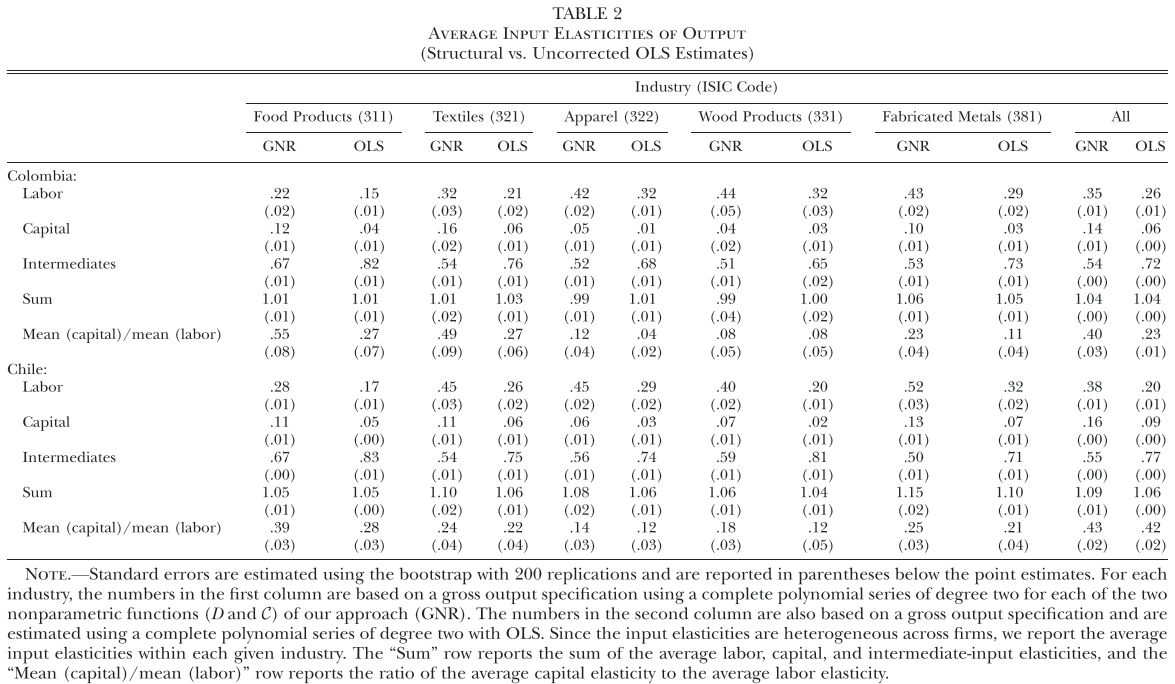
\includegraphics{images/tables/gnr-2020.png}

}

\caption{\label{fig-gnr-2020}\citet{Gandhi2020} Table 2 (GNR2020)}

\end{figure}%

\begin{table}

\caption{\label{tbl-gnr-err-stats}Fortran implementation of the
Non-Parametric GNR(2020) method to estimate production functions.
Comparison of the error standard deviation and \(\mathcal{E}\) between
the Stata code and replication data from GNR(2020), and the working data
of this paper and my own Fortran implementation code.}

\centering{

\centering
\begin{tabular}[t]{l|r|r|r|r|r|r}
\hline
\multicolumn{7}{c}{NP GNR} \\
\cline{1-7}
\multicolumn{1}{c|}{ } & \multicolumn{2}{c|}{Replication Data} & \multicolumn{4}{c}{Working Data} \\
\cline{2-3} \cline{4-7}
\multicolumn{1}{c|}{ } & \multicolumn{2}{c|}{Stata} & \multicolumn{2}{c|}{Stata} & \multicolumn{2}{c}{Fortran} \\
\cline{2-3} \cline{4-5} \cline{6-7}
  & \$\textbackslash{}mathcal\{E\}\$ & err sd & \$\textbackslash{}mathcal\{E\}\$ & err sd & \$\textbackslash{}mathcal\{E\}\$ & err sd\\
\hline
311 & 1.05 & 0.24 & 1.05 & 0.24 & 1.05 & 0.24\\
\hline
321 & 1.03 & 0.23 & 1.03 & 0.23 & 1.03 & 0.23\\
\hline
322 & 1.02 & 0.22 & 1.02 & 0.22 & 1.02 & 0.22\\
\hline
331 & 1.04 & 0.25 & 1.04 & 0.25 & 1.04 & 0.25\\
\hline
381 & 1.02 & 0.20 & 1.02 & 0.20 & 1.02 & 0.20\\
\hline
\end{tabular}

}

\end{table}%

\subsection{Cobb-Douglas Production
Function}\label{cobb-douglas-production-function}

\begin{table}

\caption{\label{tbl-fortran-gnr-cd}Fortran implementation of the
Cobb-Douglas GNR(2020) method to estimate production functions.
Comparison with Stata code and replication data from GNR(2020), and the
working data of this paper and my own Fortran implementation code.}

\centering{

\centering
\begin{tabular}[t]{l|r|r|r|r|r|r|r|r|r}
\hline
\multicolumn{10}{c}{CD GNR} \\
\cline{1-10}
\multicolumn{1}{c|}{ } & \multicolumn{3}{c|}{Replication Data} & \multicolumn{6}{c}{Working Data} \\
\cline{2-4} \cline{5-10}
\multicolumn{1}{c|}{ } & \multicolumn{3}{c|}{Stata} & \multicolumn{3}{c|}{Stata} & \multicolumn{3}{c}{Fortran} \\
\cline{2-4} \cline{5-7} \cline{8-10}
  & m & k & l & m & k & l & m & k & l\\
\hline
311 & 0.62 & 0.20 & 0.20 & 0.62 & 0.20 & 0.20 & 0.62 & 0.20 & 0.20\\
\hline
321 & 0.52 & 0.21 & 0.27 & 0.52 & 0.21 & 0.27 & 0.52 & 0.21 & 0.27\\
\hline
322 & 0.44 & 0.19 & 0.29 & 0.44 & 0.19 & 0.29 & 0.44 & 0.19 & 0.29\\
\hline
331 & 0.46 & 0.10 & 0.44 & 0.46 & 0.10 & 0.44 & 0.46 & 0.10 & 0.44\\
\hline
381 & 0.51 & 0.18 & 0.36 & 0.51 & 0.18 & 0.36 & 0.51 & 0.18 & 0.36\\
\hline
\end{tabular}

}

\end{table}%

\begin{table}

\caption{\label{tbl-gnr-err-stats-cd}Fortran implementation of the
Cobb-Douglas GNR(2020) method to estimate production functions.
Comparison of the error standard deviation and \(\mathcal{E}\) between
the Stata code and replication data from GNR(2020), and the working data
of this paper and my own Fortran implementation code.}

\centering{

\centering
\begin{tabular}[t]{l|r|r|r|r|r|r}
\hline
\multicolumn{7}{c}{CD GNR} \\
\cline{1-7}
\multicolumn{1}{c|}{ } & \multicolumn{2}{c|}{Replication Data} & \multicolumn{4}{c}{Working Data} \\
\cline{2-3} \cline{4-7}
\multicolumn{1}{c|}{ } & \multicolumn{2}{c|}{Stata} & \multicolumn{2}{c|}{Stata} & \multicolumn{2}{c}{Fortran} \\
\cline{2-3} \cline{4-5} \cline{6-7}
  & \$\textbackslash{}mathcal\{E\}\$ & err sd & \$\textbackslash{}mathcal\{E\}\$ & err sd & \$\textbackslash{}mathcal\{E\}\$ & err sd\\
\hline
311 & 1.11 & 0.33 & 1.11 & 0.33 & 1.11 & 0.33\\
\hline
321 & 1.06 & 0.30 & 1.06 & 0.30 & 1.06 & 0.30\\
\hline
322 & 1.16 & 0.43 & 1.16 & 0.43 & 1.16 & 0.43\\
\hline
331 & 1.10 & 0.39 & 1.10 & 0.39 & 1.10 & 0.39\\
\hline
381 & 1.05 & 0.29 & 1.05 & 0.29 & 1.05 & 0.29\\
\hline
\end{tabular}

}

\end{table}%

\subsection{CD GNR + trimming}\label{cd-gnr-trimming}

\begin{table}

\caption{\label{tbl-CD-GNR-trim}First State of Cobb-Douglas production
function intermediate elasticities estimates using GNR Stata estimator
and R estimator with trimmed data at 0.05. \textbf{All firms}.}

\centering{

\centering
\begin{tabular}[t]{l|l|r|r|r|l|l|l}
\hline
\multicolumn{2}{c|}{ } & \multicolumn{6}{c}{Working Data} \\
\cline{3-8}
\multicolumn{2}{c|}{ } & \multicolumn{3}{c|}{Stata} & \multicolumn{3}{c}{R} \\
\cline{3-5} \cline{6-8}
Industry & Inter. & m & \$\textbackslash{}mathcal\{E\}\$ & err sd & m & \$\textbackslash{}mathcal\{E\}\$ & err sd\\
\hline
 & Intermediates & 0.65 & 1.07 & 0.31 & 0.65 & 1.07 & 0.31\\
\cline{2-8}
 & Materials & 0.56 & 1.08 & 0.35 & 0.56 & 1.08 & 0.35\\
\cline{2-8}
\multirow[t]{-3}{*}{\raggedright\arraybackslash 311} & Deductibles & 0.56 & 1.12 & 0.39 & 0.56 & 1.12 & 0.39\\
\cline{1-8}
 & Intermediates & 0.52 & 1.06 & 0.30 & 0.52 & 1.06 & 0.3\\
\cline{2-8}
 & Materials & 0.39 & 1.12 & 0.41 & 0.39 & 1.12 & 0.41\\
\cline{2-8}
\multirow[t]{-3}{*}{\raggedright\arraybackslash 321} & Deductibles & 0.43 & 1.09 & 0.37 & 0.43 & 1.09 & 0.37\\
\cline{1-8}
 & Intermediates & 0.45 & 1.13 & 0.41 & 0.45 & 1.13 & 0.41\\
\cline{2-8}
 & Materials & 0.37 & 1.15 & 0.45 & 0.37 & 1.15 & 0.45\\
\cline{2-8}
\multirow[t]{-3}{*}{\raggedright\arraybackslash 322} & Deductibles & 0.37 & 1.15 & 0.45 & 0.37 & 1.15 & 0.45\\
\cline{1-8}
 & Intermediates & 0.47 & 1.09 & 0.38 & 0.47 & 1.09 & 0.38\\
\cline{2-8}
 & Materials & 0.35 & 1.14 & 0.48 & 0.35 & 1.14 & 0.48\\
\cline{2-8}
\multirow[t]{-3}{*}{\raggedright\arraybackslash 331} & Deductibles & 0.39 & 1.12 & 0.43 & 0.39 & 1.12 & 0.43\\
\cline{1-8}
 & Intermediates & 0.51 & 1.05 & 0.29 & 0.51 & 1.05 & 0.29\\
\cline{2-8}
 & Materials & 0.37 & 1.09 & 0.39 & 0.37 & 1.09 & 0.39\\
\cline{2-8}
\multirow[t]{-3}{*}{\raggedright\arraybackslash 381} & Deductibles & 0.41 & 1.07 & 0.35 & 0.41 & 1.07 & 0.35\\
\hline
\end{tabular}

}

\end{table}%

\subsection{CD GNR + Trimming +
Corporations}\label{cd-gnr-trimming-corporations}

\begin{table}

\caption{\label{tbl-CD-GNR-trim-corps}First State of Cobb-Douglas
production function intermediate elasticities estimates using GNR Stata
estimator and R estimator with trimmed data at 0.05. \textbf{Only
Corporations}.}

\centering{

\centering
\begin{tabular}[t]{l|l|r|r|r|l|l|l}
\hline
\multicolumn{2}{c|}{ } & \multicolumn{6}{c}{Working Data} \\
\cline{3-8}
\multicolumn{2}{c|}{ } & \multicolumn{3}{c|}{Stata.} & \multicolumn{3}{c}{R} \\
\cline{3-5} \cline{6-8}
Industry & Inter. & m & \$\textbackslash{}mathcal\{E\}\$ & err sd & m & \$\textbackslash{}mathcal\{E\}\$ & err sd\\
\hline
 & Intermediates & 0.67 & 1.06 & 0.28 & 0.67 & 1.06 & 0.28\\
\cline{2-8}
 & Materials & 0.55 & 1.08 & 0.35 & 0.55 & 1.08 & 0.35\\
\cline{2-8}
\multirow[t]{-3}{*}{\raggedright\arraybackslash 311} & Deductibles & 0.57 & 1.09 & 0.35 & 0.57 & 1.09 & 0.35\\
\cline{1-8}
 & Intermediates & 0.51 & 1.03 & 0.24 & 0.51 & 1.03 & 0.24\\
\cline{2-8}
 & Materials & 0.35 & 1.09 & 0.37 & 0.35 & 1.09 & 0.37\\
\cline{2-8}
\multirow[t]{-3}{*}{\raggedright\arraybackslash 321} & Deductibles & 0.40 & 1.07 & 0.33 & 0.4 & 1.07 & 0.33\\
\cline{1-8}
 & Intermediates & 0.25 & 1.59 & 0.82 & 0.25 & 1.59 & 0.82\\
\cline{2-8}
 & Materials & 0.31 & 1.11 & 0.41 & 0.31 & 1.11 & 0.41\\
\cline{2-8}
\multirow[t]{-3}{*}{\raggedright\arraybackslash 322} & Deductibles & 0.34 & 1.09 & 0.38 & 0.34 & 1.09 & 0.38\\
\cline{1-8}
 & Intermediates & 0.50 & 1.03 & 0.24 & 0.5 & 1.03 & 0.24\\
\cline{2-8}
 & Materials & 0.29 & 1.09 & 0.42 & 0.29 & 1.09 & 0.42\\
\cline{2-8}
\multirow[t]{-3}{*}{\raggedright\arraybackslash 331} & Deductibles & 0.37 & 1.05 & 0.30 & 0.37 & 1.05 & 0.3\\
\cline{1-8}
 & Intermediates & 0.54 & 1.04 & 0.27 & 0.54 & 1.04 & 0.27\\
\cline{2-8}
 & Materials & 0.37 & 1.09 & 0.40 & 0.37 & 1.09 & 0.4\\
\cline{2-8}
\multirow[t]{-3}{*}{\raggedright\arraybackslash 381} & Deductibles & 0.41 & 1.08 & 0.37 & 0.41 & 1.08 & 0.37\\
\hline
\end{tabular}

}

\end{table}%

\subsection{CD GNR + Trimming + Measurement
Error}\label{cd-gnr-trimming-measurement-error}

\begin{table}

\caption{\label{tbl-CD-GNR-me}First State of Cobb-Douglas production
function intermediate elasticities estimates using GNR Stata estimator
and R estimator with trimmed data at 0.05. \textbf{Corporations
vs.~All}. \(\varepsilon\) is the \textbf{measurement error}.}

\centering{

\centering
\begin{tabular}[t]{l|l|l|l|l|l|l|l}
\hline
\multicolumn{2}{c|}{ } & \multicolumn{6}{c}{Working Data (R)} \\
\cline{3-8}
\multicolumn{2}{c|}{ } & \multicolumn{3}{c|}{Corps.} & \multicolumn{3}{c}{All} \\
\cline{3-5} \cline{6-8}
Industry & Inter. & m & \$\textbackslash{}mathcal\{E\}\$ & err sd & m & \$\textbackslash{}mathcal\{E\}\$ & err sd\\
\hline
 & Intermediates & 0.71 & 1 & 0.28 & 0.69 & 1 & 0.31\\
\cline{2-8}
 & Materials & 0.6 & 1 & 0.35 & 0.61 & 1 & 0.35\\
\cline{2-8}
\multirow[t]{-3}{*}{\raggedright\arraybackslash 311} & Deductibles & 0.62 & 1 & 0.35 & 0.63 & 1 & 0.39\\
\cline{1-8}
 & Intermediates & 0.53 & 1 & 0.24 & 0.55 & 1 & 0.3\\
\cline{2-8}
 & Materials & 0.39 & 1 & 0.37 & 0.43 & 1 & 0.41\\
\cline{2-8}
\multirow[t]{-3}{*}{\raggedright\arraybackslash 321} & Deductibles & 0.43 & 1 & 0.33 & 0.47 & 1 & 0.37\\
\cline{1-8}
 & Intermediates & 0.4 & 1 & 0.82 & 0.51 & 1 & 0.41\\
\cline{2-8}
 & Materials & 0.35 & 1 & 0.41 & 0.42 & 1 & 0.45\\
\cline{2-8}
\multirow[t]{-3}{*}{\raggedright\arraybackslash 322} & Deductibles & 0.37 & 1 & 0.38 & 0.43 & 1 & 0.45\\
\cline{1-8}
 & Intermediates & 0.51 & 1 & 0.24 & 0.51 & 1 & 0.38\\
\cline{2-8}
 & Materials & 0.32 & 1 & 0.42 & 0.4 & 1 & 0.48\\
\cline{2-8}
\multirow[t]{-3}{*}{\raggedright\arraybackslash 331} & Deductibles & 0.39 & 1 & 0.3 & 0.44 & 1 & 0.43\\
\cline{1-8}
 & Intermediates & 0.56 & 1 & 0.27 & 0.53 & 1 & 0.29\\
\cline{2-8}
 & Materials & 0.41 & 1 & 0.4 & 0.41 & 1 & 0.39\\
\cline{2-8}
\multirow[t]{-3}{*}{\raggedright\arraybackslash 381} & Deductibles & 0.44 & 1 & 0.37 & 0.44 & 1 & 0.35\\
\hline
\end{tabular}

}

\end{table}%

\begin{table}

\caption{\label{tbl-CD-GNR-me-ev}First State of Cobb-Douglas production
function intermediate elasticities estimates using GNR Stata estimator
and R estimator with trimmed data at 0.05. \textbf{Corporations
vs.~All}. \(\varepsilon\) is the \textbf{measurement error}. Top evading
industries.}

\centering{

\centering
\begin{tabular}[t]{l|l|l|l|l|l|l|l}
\hline
\multicolumn{2}{c|}{ } & \multicolumn{6}{c}{Working Data (R)} \\
\cline{3-8}
\multicolumn{2}{c|}{ } & \multicolumn{3}{c|}{Corps.} & \multicolumn{3}{c}{All} \\
\cline{3-5} \cline{6-8}
Industry & Inter. & m & \$\textbackslash{}mathcal\{E\}\$ & err sd & m & \$\textbackslash{}mathcal\{E\}\$ & err sd\\
\hline
 & Intermediates & 0.4 & 1 & 0.82 & 0.51 & 1 & 0.41\\
\cline{2-8}
 & Materials & 0.35 & 1 & 0.41 & 0.42 & 1 & 0.45\\
\cline{2-8}
\multirow[t]{-3}{*}{\raggedright\arraybackslash 322} & Deductibles & 0.37 & 1 & 0.38 & 0.43 & 1 & 0.45\\
\cline{1-8}
 & Intermediates & 0.41 & 1 & 0.41 & 0.37 & 1 & 0.54\\
\cline{2-8}
 & Materials & 0.24 & 1 & 0.61 & 0.28 & 1 & 0.62\\
\cline{2-8}
\multirow[t]{-3}{*}{\raggedright\arraybackslash 369} & Deductibles & 0.35 & 1 & 0.41 & 0.34 & 1 & 0.46\\
\cline{1-8}
 & Intermediates & 0.51 & 1 & 0.24 & 0.51 & 1 & 0.38\\
\cline{2-8}
 & Materials & 0.32 & 1 & 0.42 & 0.4 & 1 & 0.48\\
\cline{2-8}
\multirow[t]{-3}{*}{\raggedright\arraybackslash 331} & Deductibles & 0.39 & 1 & 0.3 & 0.44 & 1 & 0.43\\
\cline{1-8}
 & Intermediates & 0.53 & 1 & 0.24 & 0.55 & 1 & 0.3\\
\cline{2-8}
 & Materials & 0.39 & 1 & 0.37 & 0.43 & 1 & 0.41\\
\cline{2-8}
\multirow[t]{-3}{*}{\raggedright\arraybackslash 321} & Deductibles & 0.43 & 1 & 0.33 & 0.47 & 1 & 0.37\\
\cline{1-8}
 & Intermediates & 0.55 & 1 & 0.3 & 0.55 & 1 & 0.32\\
\cline{2-8}
 & Materials & 0.34 & 1 & 0.63 & 0.35 & 1 & 0.62\\
\cline{2-8}
\multirow[t]{-3}{*}{\raggedright\arraybackslash 351} & Deductibles & 0.44 & 1 & 0.4 & 0.44 & 1 & 0.41\\
\hline
\end{tabular}

}

\end{table}%

\subsection{Industry Characteristics}\label{industry-characteristics}

\begin{table}

\caption{\label{tbl-good-guys}Intermediate elasticities for different
groups of firms using GNR method assuming a CD functional form. Data
trimmed at 0.05 of the intermediates share cost of gross output.
\(\varepsilon\) is defined as \textbf{measurement error}.}

\centering{

\centering
\begin{tabular}[t]{l|l|l|l|l|l}
\hline
\multicolumn{2}{c|}{ } & \multicolumn{4}{c}{m} \\
\cline{3-6}
Inds. & Intermediate & Corps. & Exp. & Imp. & All\\
\hline
311 & Materials & 0.6 & 0.61 & 0.35 & 0.61\\
\cline{1-6}
312 & Materials & 0.58 & 0.57 & 0.49 & 0.58\\
\cline{1-6}
313 & Materials & 0.29 & 0.35 & 0.36 & 0.31\\
\cline{1-6}
321 & Materials & 0.39 & 0.44 & 0.37 & 0.43\\
\cline{1-6}
322 & Materials & 0.35 & 0.42 & 0.41 & 0.42\\
\cline{1-6}
323 & Materials & 0.56 & 0.47 & 0.22 & 0.48\\
\cline{1-6}
324 & Materials & 0.43 & 0.46 & 0.22 & 0.46\\
\cline{1-6}
331 & Materials & 0.32 & 0.41 & 0.42 & 0.4\\
\cline{1-6}
332 & Materials & 0.36 & 0.35 & 0.42 & 0.35\\
\hline
\end{tabular}

}

\end{table}%

\begin{table}

\caption{\label{tbl-industry-characteristics}One side test of tax
evasion through inputs overreporting. Different non-evaders groups used
as reference.}

\centering{

\centering
\begin{tabular}[t]{l|l|l|l|l|l|l}
\hline
\multicolumn{1}{c|}{ } & \multicolumn{2}{c|}{Corporations} & \multicolumn{2}{c|}{Exporters} & \multicolumn{2}{c}{Importers} \\
\cline{2-3} \cline{4-5} \cline{6-7}
Inds. & Materials & Deductibles & Materials & Deductibles & Materials & Deductibles\\
\hline
311 & 0.1111 (0.0045)*** & 0.0294 (0.005)*** & -0.1489 (0.0124) & -0.0416 (0.0056) & -0.2007 (0.0124) & -0.1147 (0.0056)\\
\hline
312 & -0.0098 (0.0158) & 0.0251 (0.0115)** & 0.0516 (0.0257)** & 0.0648 (0.0127)*** & -0.1104 (0.0257) & 0.0707 (0.0127)***\\
\hline
313 & 0.0659 (0.0123)*** & 0.0377 (0.0111)*** & 0.2794 (0.0123)*** & 0.3439 (0.0111)*** & 0.1218 (0.0123)*** & 0.0935 (0.0111)***\\
\hline
321 & 0.1262 (0.0078)*** & 0.0885 (0.007)*** & 0.0604 (0.0111)*** & 0.115 (0.0079)*** & 0.016 (0.0111)* & 0.0247 (0.0079)***\\
\hline
322 & 1.27 (0.0068)*** & 0.6404 (0.0068)*** & 0.1215 (0.0145)*** & 0.1103 (0.009)*** & -0.1187 (0.0145) & -0.0914 (0.009)\\
\hline
323 & -0.1534 (0.0133) & -0.1635 (0.0137) & -0.181 (0.0179) & -0.1646 (0.0152) & -0.1544 (0.0179) & -0.1542 (0.0152)\\
\hline
324 & 0.0664 (0.0086)*** & 0.0578 (0.0084)*** & -0.1202 (0.0188) & -0.098 (0.0099) & -0.0588 (0.0188) & -0.0537 (0.0099)\\
\hline
331 & 0.2177 (0.0154)*** & 0.1205 (0.0139)*** & 0.086 (0.0198)*** & 0.1038 (0.0148)*** & -0.0852 (0.0198) & -0.0367 (0.0148)\\
\hline
332 & -0.028 (0.0136) & -0.0284 (0.0127) & -0.1286 (0.0142) & -0.1522 (0.0133) & -0.2887 (0.0142) & -0.2709 (0.0133)\\
\hline
\end{tabular}

}

\end{table}%

\section{CD GNR Intermediates}\label{cd-gnr-intermediates}

Observations with value of zero for some intermediates were driving down
the estimates of the output elasticity of intermediates. This is a
common problem when using data from surveys. To avoid this problem, I
trimmed the observations with a share of intermediates below 0.05.

These observations increase the variance of the error term, which in
turn increases the value of \(\mathcal{E}\). The higher the value of
\(\mathcal{E}\), the lower the value of the elasticity of intermediates.

Figure~\ref{fig-cutoff} show that at when trimming observations with a
share of intermediates below 0.05, the estimates of \(\mathcal{E}\) and
the output elasticity of intermediates start to stabilize. That is the
changes in the values of these variables are small. In addition,
Figure~\ref{fig-cutoff-drop} shows that at this threshold, the change in
percentage of observations dropped is also small.

A more detailed picture of this is displayed in
\textbf{?@tbl-cd-gnr-inter-trim}. The table compares the estimates of
the output elasticity of intermediates and other statistics of the first
stage of GNR(2020) assuming a Cobb-Douglas Production Function for
different definitions of intermediates and different thresholds for
trimming observations.

\begin{figure}

\centering{

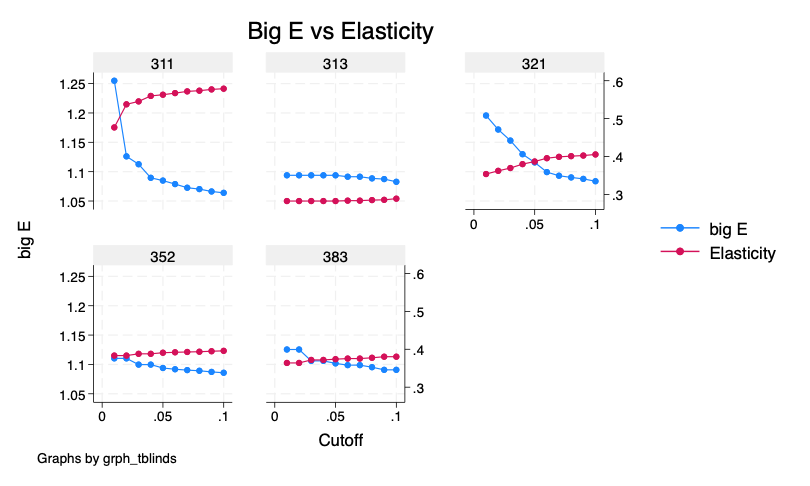
\includegraphics{images/graphs/trim-bigE-inds.png}

}

\caption{\label{fig-cutoff}Estimates of \(\mathcal{E}\) and the output
elasticity of intermediates (raw materials) trimming observations with a
share of intermediates below different thresholds going from 0.01 to 0.1
. The elasticities of intermediates were estimated assuming a
Cobb-Douglas production function using the first stage of GNR(2020).}

\end{figure}%

\begin{figure}

\centering{

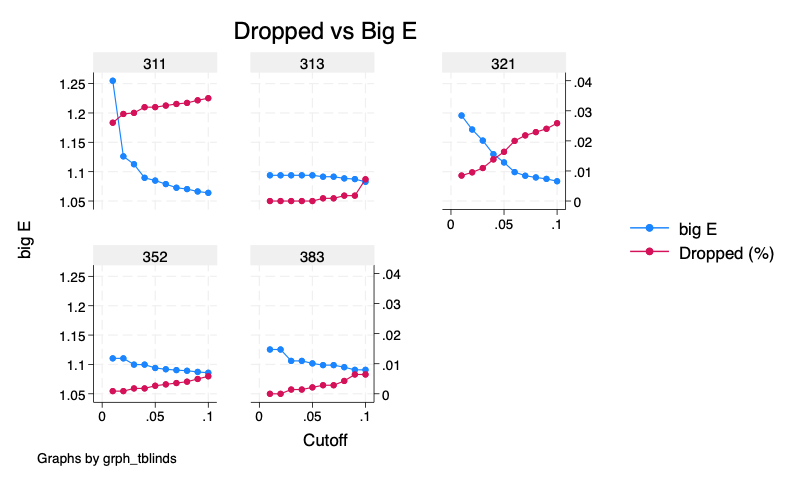
\includegraphics{images/graphs/trim-drop-all.png}

}

\caption{\label{fig-cutoff-drop}Estimates of \(\mathcal{E}\) and
percentage of observations dropped by trimming observations with a share
of intermediates (raw materials) below different thresholds going from
0.01 to 0.1 . The elasticities of intermediates were estimated assuming
a Cobb-Douglas production function using the first stage of GNR(2020).}

\end{figure}%

\begin{table}

\caption{\label{tbl-cd-gnr-inter}Estimates of Cobb-Douglas Production
Function parameters using GNR(2020) and statistics of the first stage
for different definitions of intermediates. \emph{m s e} stands for raw
materials, services, and energy, \emph{mats} for raw materials, and
\emph{ded} for deductible intermediates (raw materials, electricity,
fuels, and repair and maintenance services). Observations were trimmed
below a share of intermediates of 0.05.}

\centering{

\centering
\begin{tabular}[t]{l|l|r|r|r|r|r|r|r}
\hline
Ind. & Inter. & m & l & k & bigE & si\_mean & err\_mean & err\_sd\\
\hline
 & m\_s\_e & 0.6488 & 0.1827 & 0.1832 & 1.0652 & 0.7219 & 0 & 0.3091\\
\cline{2-9}
 & mats & 0.5630 & 0.2084 & 0.2443 & 1.0848 & 0.6416 & 0 & 0.3470\\
\cline{2-9}
\multirow[t]{-3}{*}{\raggedright\arraybackslash 311} & ded & 0.5567 & 0.2194 & 0.2337 & 1.1232 & 0.6631 & 0 & 0.3948\\
\cline{1-9}
 & m\_s\_e & 0.5183 & 0.2658 & 0.2088 & 1.0557 & 0.5689 & 0 & 0.2996\\
\cline{2-9}
 & mats & 0.3869 & 0.3412 & 0.2604 & 1.1158 & 0.4633 & 0 & 0.4136\\
\cline{2-9}
\multirow[t]{-3}{*}{\raggedright\arraybackslash 321} & ded & 0.4273 & 0.3237 & 0.2470 & 1.0934 & 0.4949 & 0 & 0.3720\\
\cline{1-9}
 & m\_s\_e & 0.5749 & 0.2133 & 0.2415 & 1.0437 & 0.6201 & 0 & 0.2718\\
\cline{2-9}
 & mats & 0.3909 & 0.2858 & 0.3527 & 1.0940 & 0.4574 & 0 & 0.3922\\
\cline{2-9}
\multirow[t]{-3}{*}{\raggedright\arraybackslash 352} & ded & 0.4114 & 0.2797 & 0.3360 & 1.0877 & 0.4756 & 0 & 0.3746\\
\cline{1-9}
 & m\_s\_e & 0.4324 & 0.1658 & 0.3086 & 1.0721 & 0.4893 & 0 & 0.3479\\
\cline{2-9}
 & mats & 0.2826 & 0.2943 & 0.3395 & 1.0938 & 0.3347 & 0 & 0.4104\\
\cline{2-9}
\multirow[t]{-3}{*}{\raggedright\arraybackslash 313} & ded & 0.3216 & 0.2912 & 0.3203 & 1.0767 & 0.3699 & 0 & 0.3726\\
\cline{1-9}
 & m\_s\_e & 0.5261 & 0.3666 & 0.1892 & 1.0445 & 0.5694 & 0 & 0.2786\\
\cline{2-9}
 & mats & 0.3739 & 0.4889 & 0.2523 & 1.1018 & 0.4427 & 0 & 0.4069\\
\cline{2-9}
\multirow[t]{-3}{*}{\raggedright\arraybackslash 383} & ded & 0.4015 & 0.4532 & 0.2427 & 1.0891 & 0.4655 & 0 & 0.3798\\
\hline
\end{tabular}

}

\end{table}%

\section{Density}\label{density}

\begin{figure}

\begin{minipage}{\linewidth}

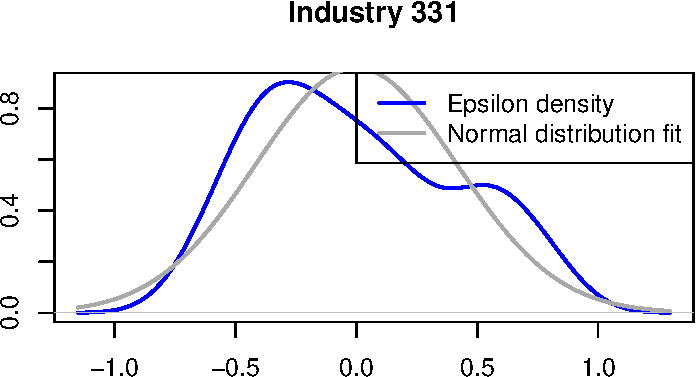
\includegraphics{Tax-Prod_files/figure-pdf/unnamed-chunk-44-1.pdf}

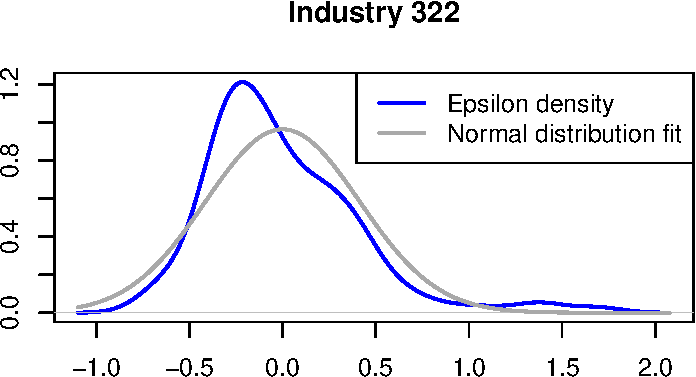
\includegraphics{Tax-Prod_files/figure-pdf/unnamed-chunk-44-2.pdf}

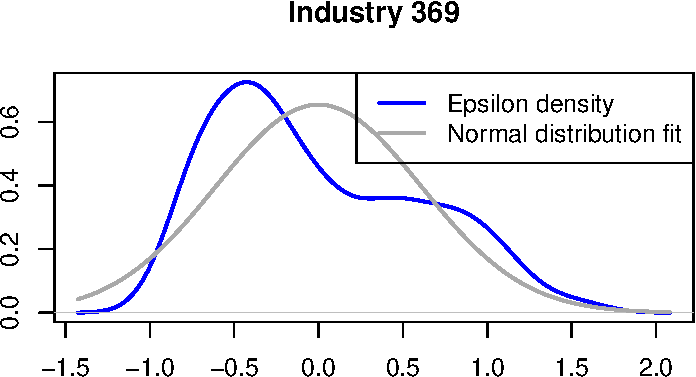
\includegraphics{Tax-Prod_files/figure-pdf/unnamed-chunk-44-3.pdf}

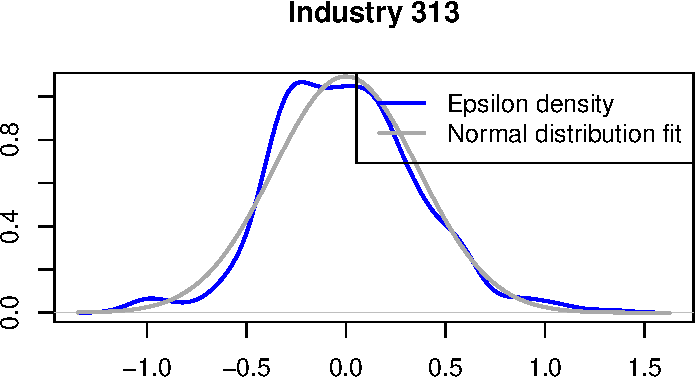
\includegraphics{Tax-Prod_files/figure-pdf/unnamed-chunk-44-4.pdf}

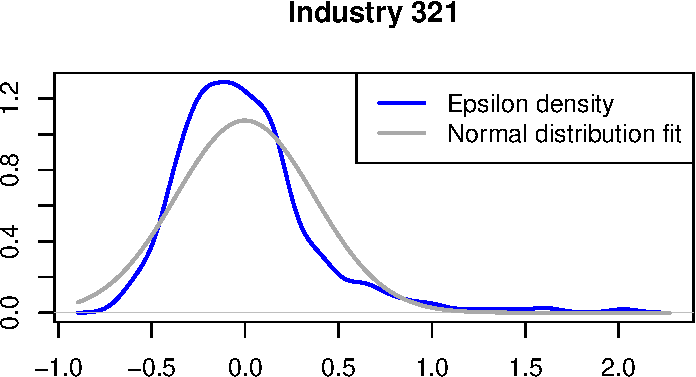
\includegraphics{Tax-Prod_files/figure-pdf/unnamed-chunk-44-5.pdf}

\end{minipage}%

\end{figure}%




\end{document}
